\section{Experimental work/ analytical investigation/ design}

\textbf{Experimental workflow}

The experiment workflow is outlined in the diagram below, detailing the sequential steps from data collection to iterative improvement of the model.

\begin{center}

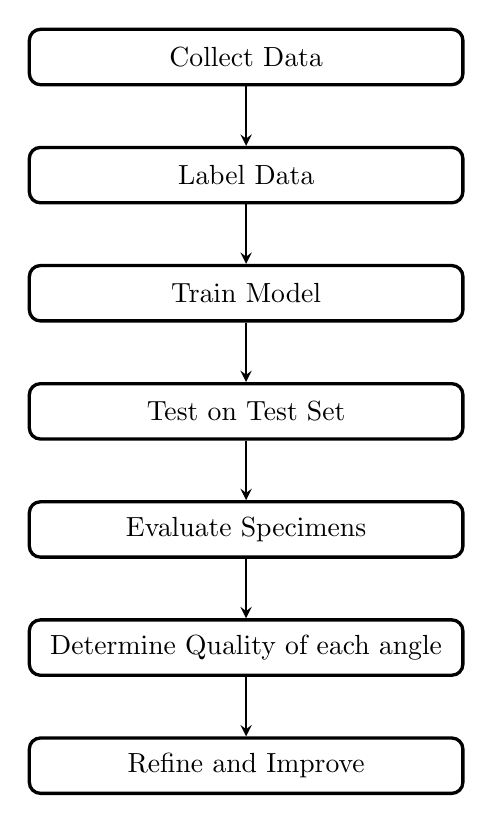
\begin{tikzpicture}[node distance=1.5cm,
    box/.style={
        rectangle,
        rounded corners,
        draw=black, very thick,
        text width=15em,
        minimum height=2em,
        text centered},
    arrow/.style={
        thick,
        ->,
        >=stealth}
    ]

    \node (collect) [box] {Collect Data};
    \node (mix) [box, below of=collect] {Label Data};
    \node (train) [box, below of=mix] {Train Model};
    \node (test) [box, below of=train] {Test on Test Set};
    \node (evaluate) [box, below of=test] {Evaluate Specimens};
    \node (rate) [box, below of=evaluate] {Determine Quality of each angle};
    \node (improve) [box, below of=rate] {Refine and Improve};
    
    \draw [arrow] (collect) -- (mix);
    \draw [arrow] (mix) -- (train);
    \draw [arrow] (train) -- (test);
    \draw [arrow] (test) -- (evaluate);
    \draw [arrow] (evaluate) -- (rate);
    \draw [arrow] (rate) -- (improve);
    
    \end{tikzpicture}
\end{center}



\subsection{Data Collection}
The first essential step for deep learning is data collection. In this experiment, pre-prepared paraffin-embedded tissue sections (fish ovary tissues) were used. These sections were placed on an HM355s automatic microtome, and slicing operations were performed according to different cutting angles as specified in the microtome's manual. The cutting data was recorded meticulously.

%在这不要提三个点的鱼的肺泡组织,在后面作为模型二次验证和增强使用。

The schematic diagram of the microtome (taking a tooth as an example) is shown in \autoref{fig:cutting_machine} \cite{4.1}.

\begin{figure}[htbp]
    \centering
    \begin{minipage}{0.48\textwidth}
        \centering
        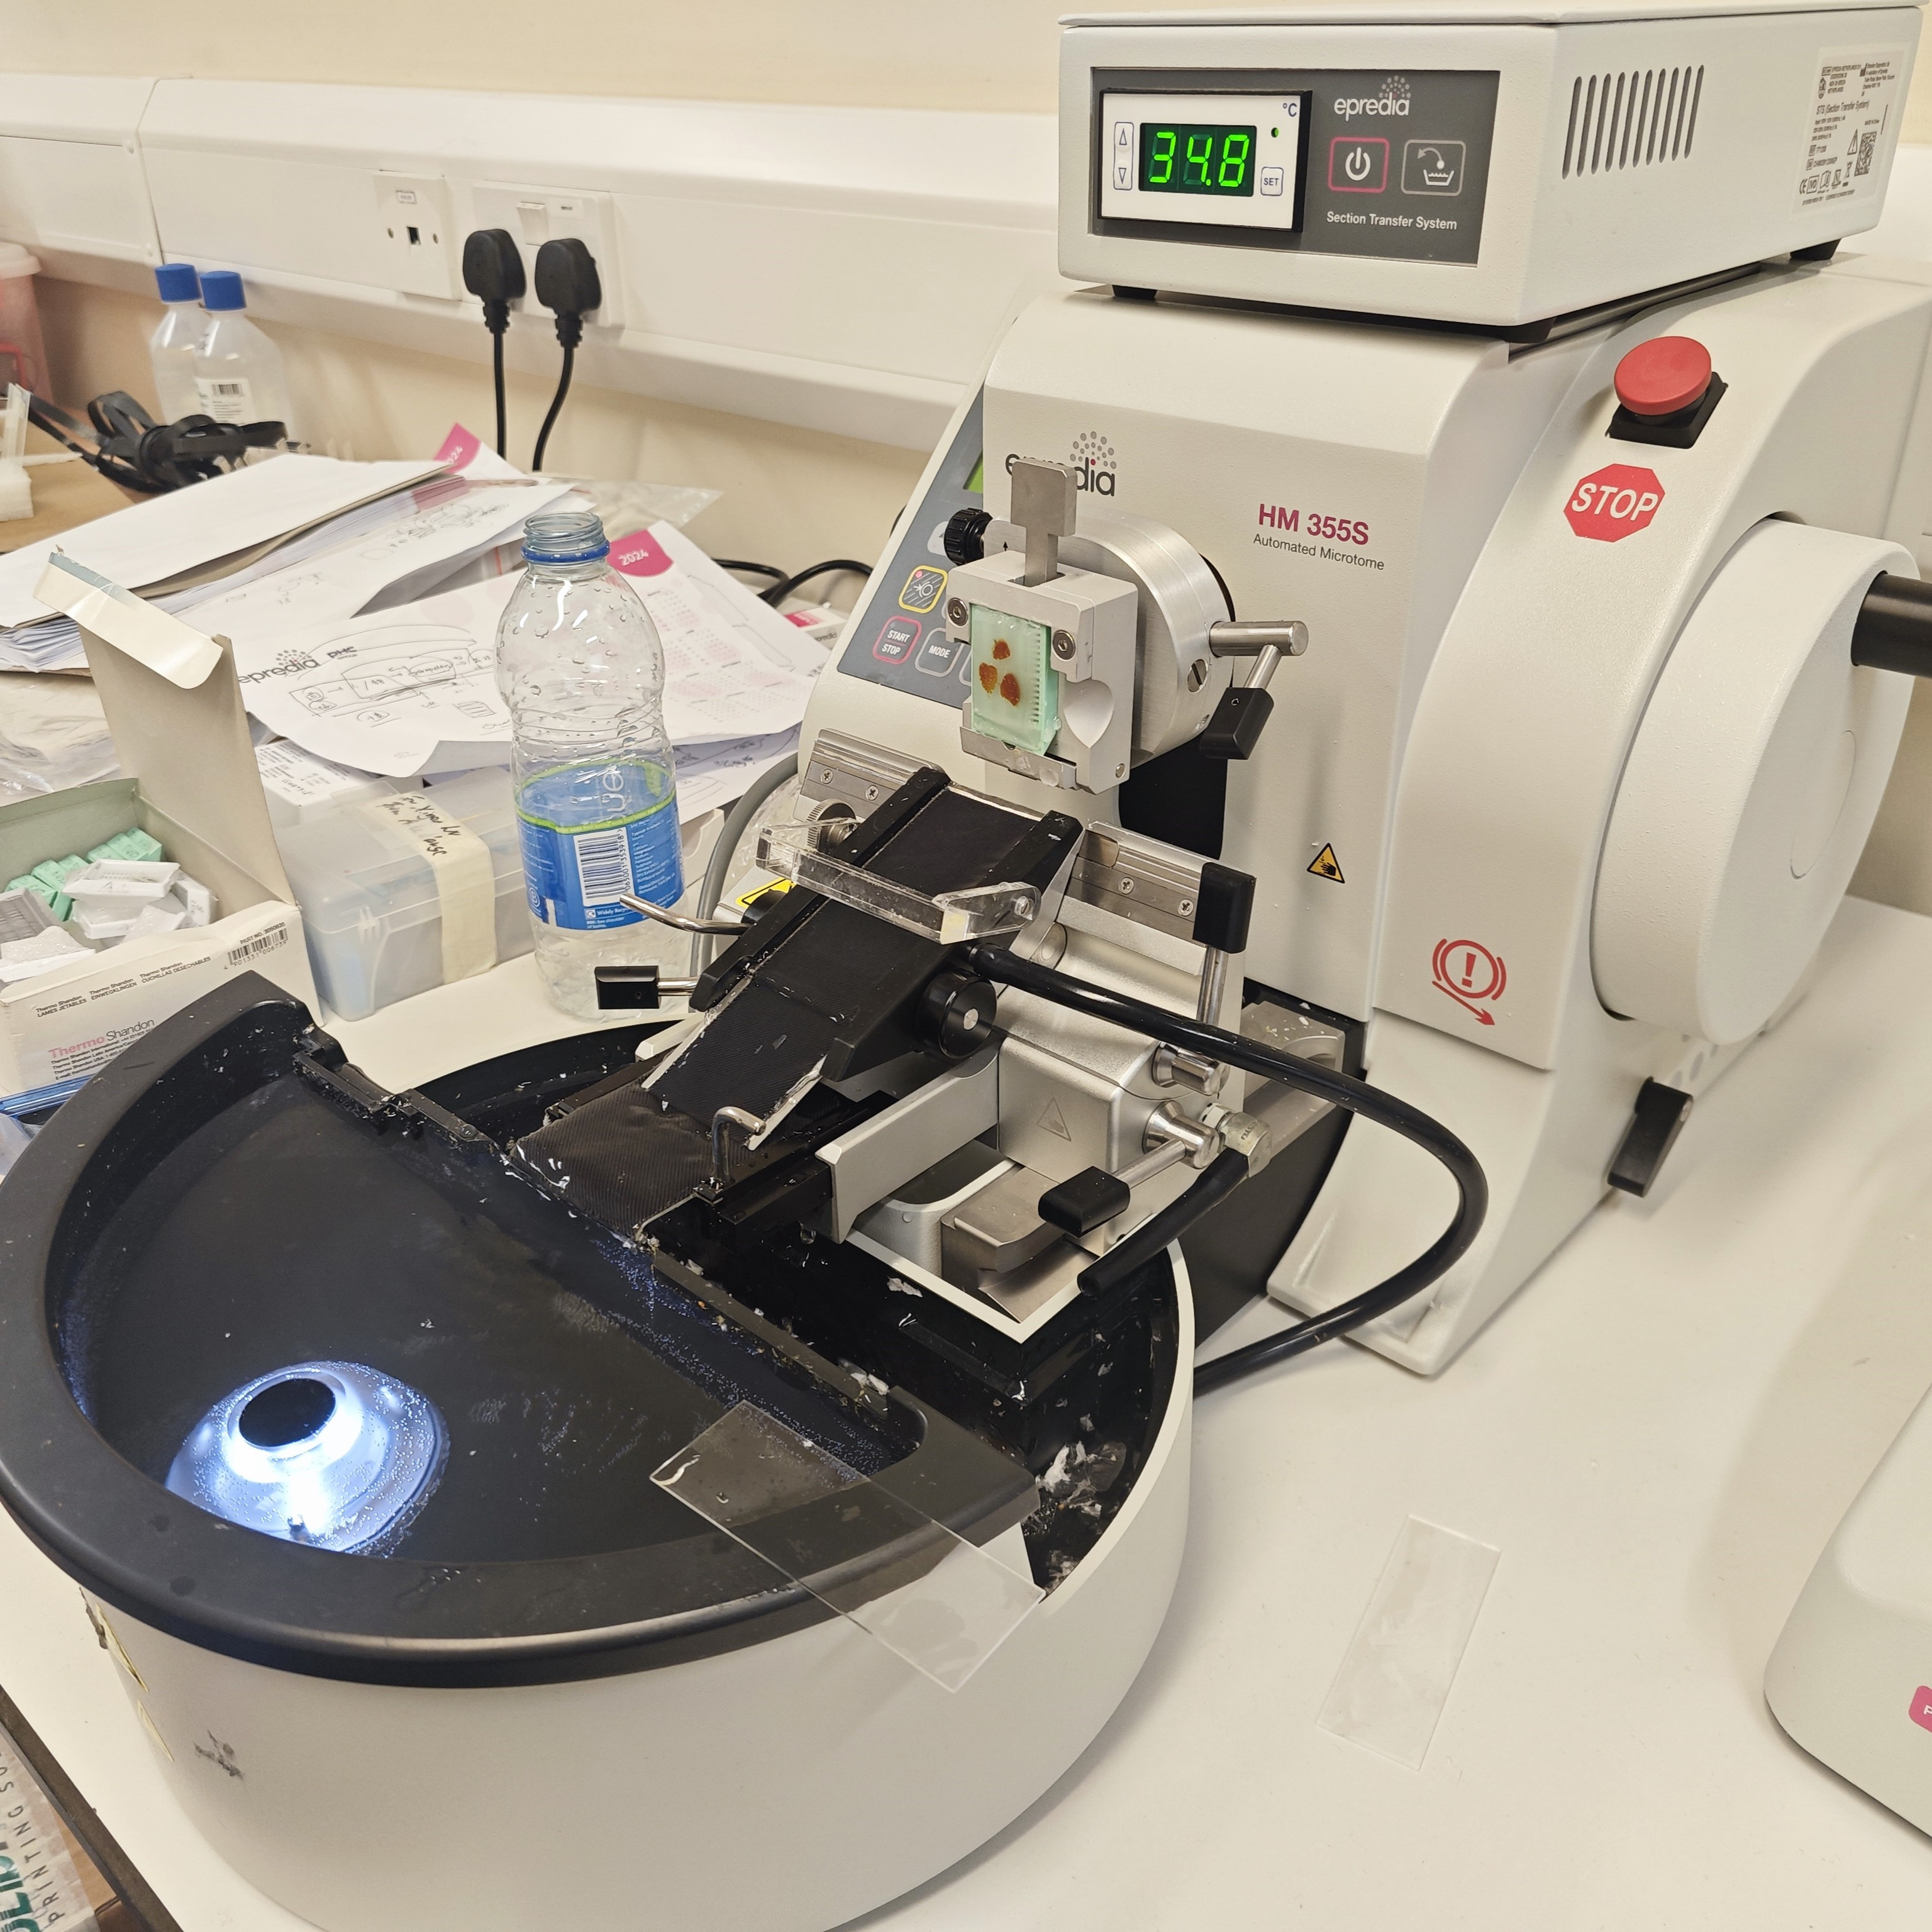
\includegraphics[width=\textwidth]{./fig/machine.jpg}
        \caption{Microtome}
        \label{fig:machine}
    \end{minipage}
    \begin{minipage}{0.48\textwidth}
        \centering
        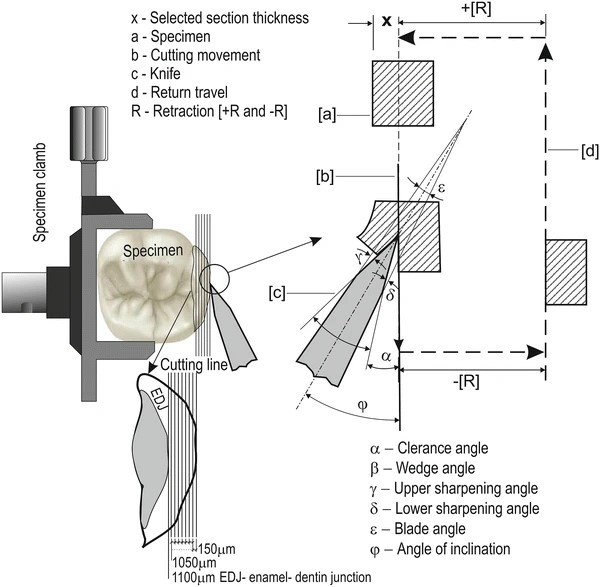
\includegraphics[width=\textwidth]{./fig/10266_2018_353_Fig1_HTML.jpg}
        \caption{Working principle of the microtome}
        \label{fig:cutting_machine}
    \end{minipage}
\end{figure}
% https://link.springer.com/article/10.1007/s10266-018-0353-6



% 在切削过程中,从切角为8度开始(如\autoref{fig:machine}中的angle of inclination),每次增加0.5度,直到切角为12度。切片机在切片过程中保持给进速度为25,厚度为1。

In the experiment, the microtome was configured with the following parameters: the mode was set to continuous, the feed rate was 5.0, the trimming value was 25, the speed was set at 32, the water flow rate was 7.5, and the water temperature was approximately 36 degrees Celsius. The cutting angle was adjusted between 8 to 12 degrees.

The biological tissues used for sectioning are shown in Figure \ref{label:sample}. After sectioning, the different types of tissue sections were placed on slides as depicted in Figure \ref{fig:采集样本}. Once dried, these slides were transferred under a VHX7000 microscope for imaging. Each sample was photographed under the microscope to capture electronic image data, as shown in Figure \ref{fig:显微镜}.

\begin{figure}[htbp]
    \centering
    \begin{minipage}{0.3\textwidth}
        \centering
        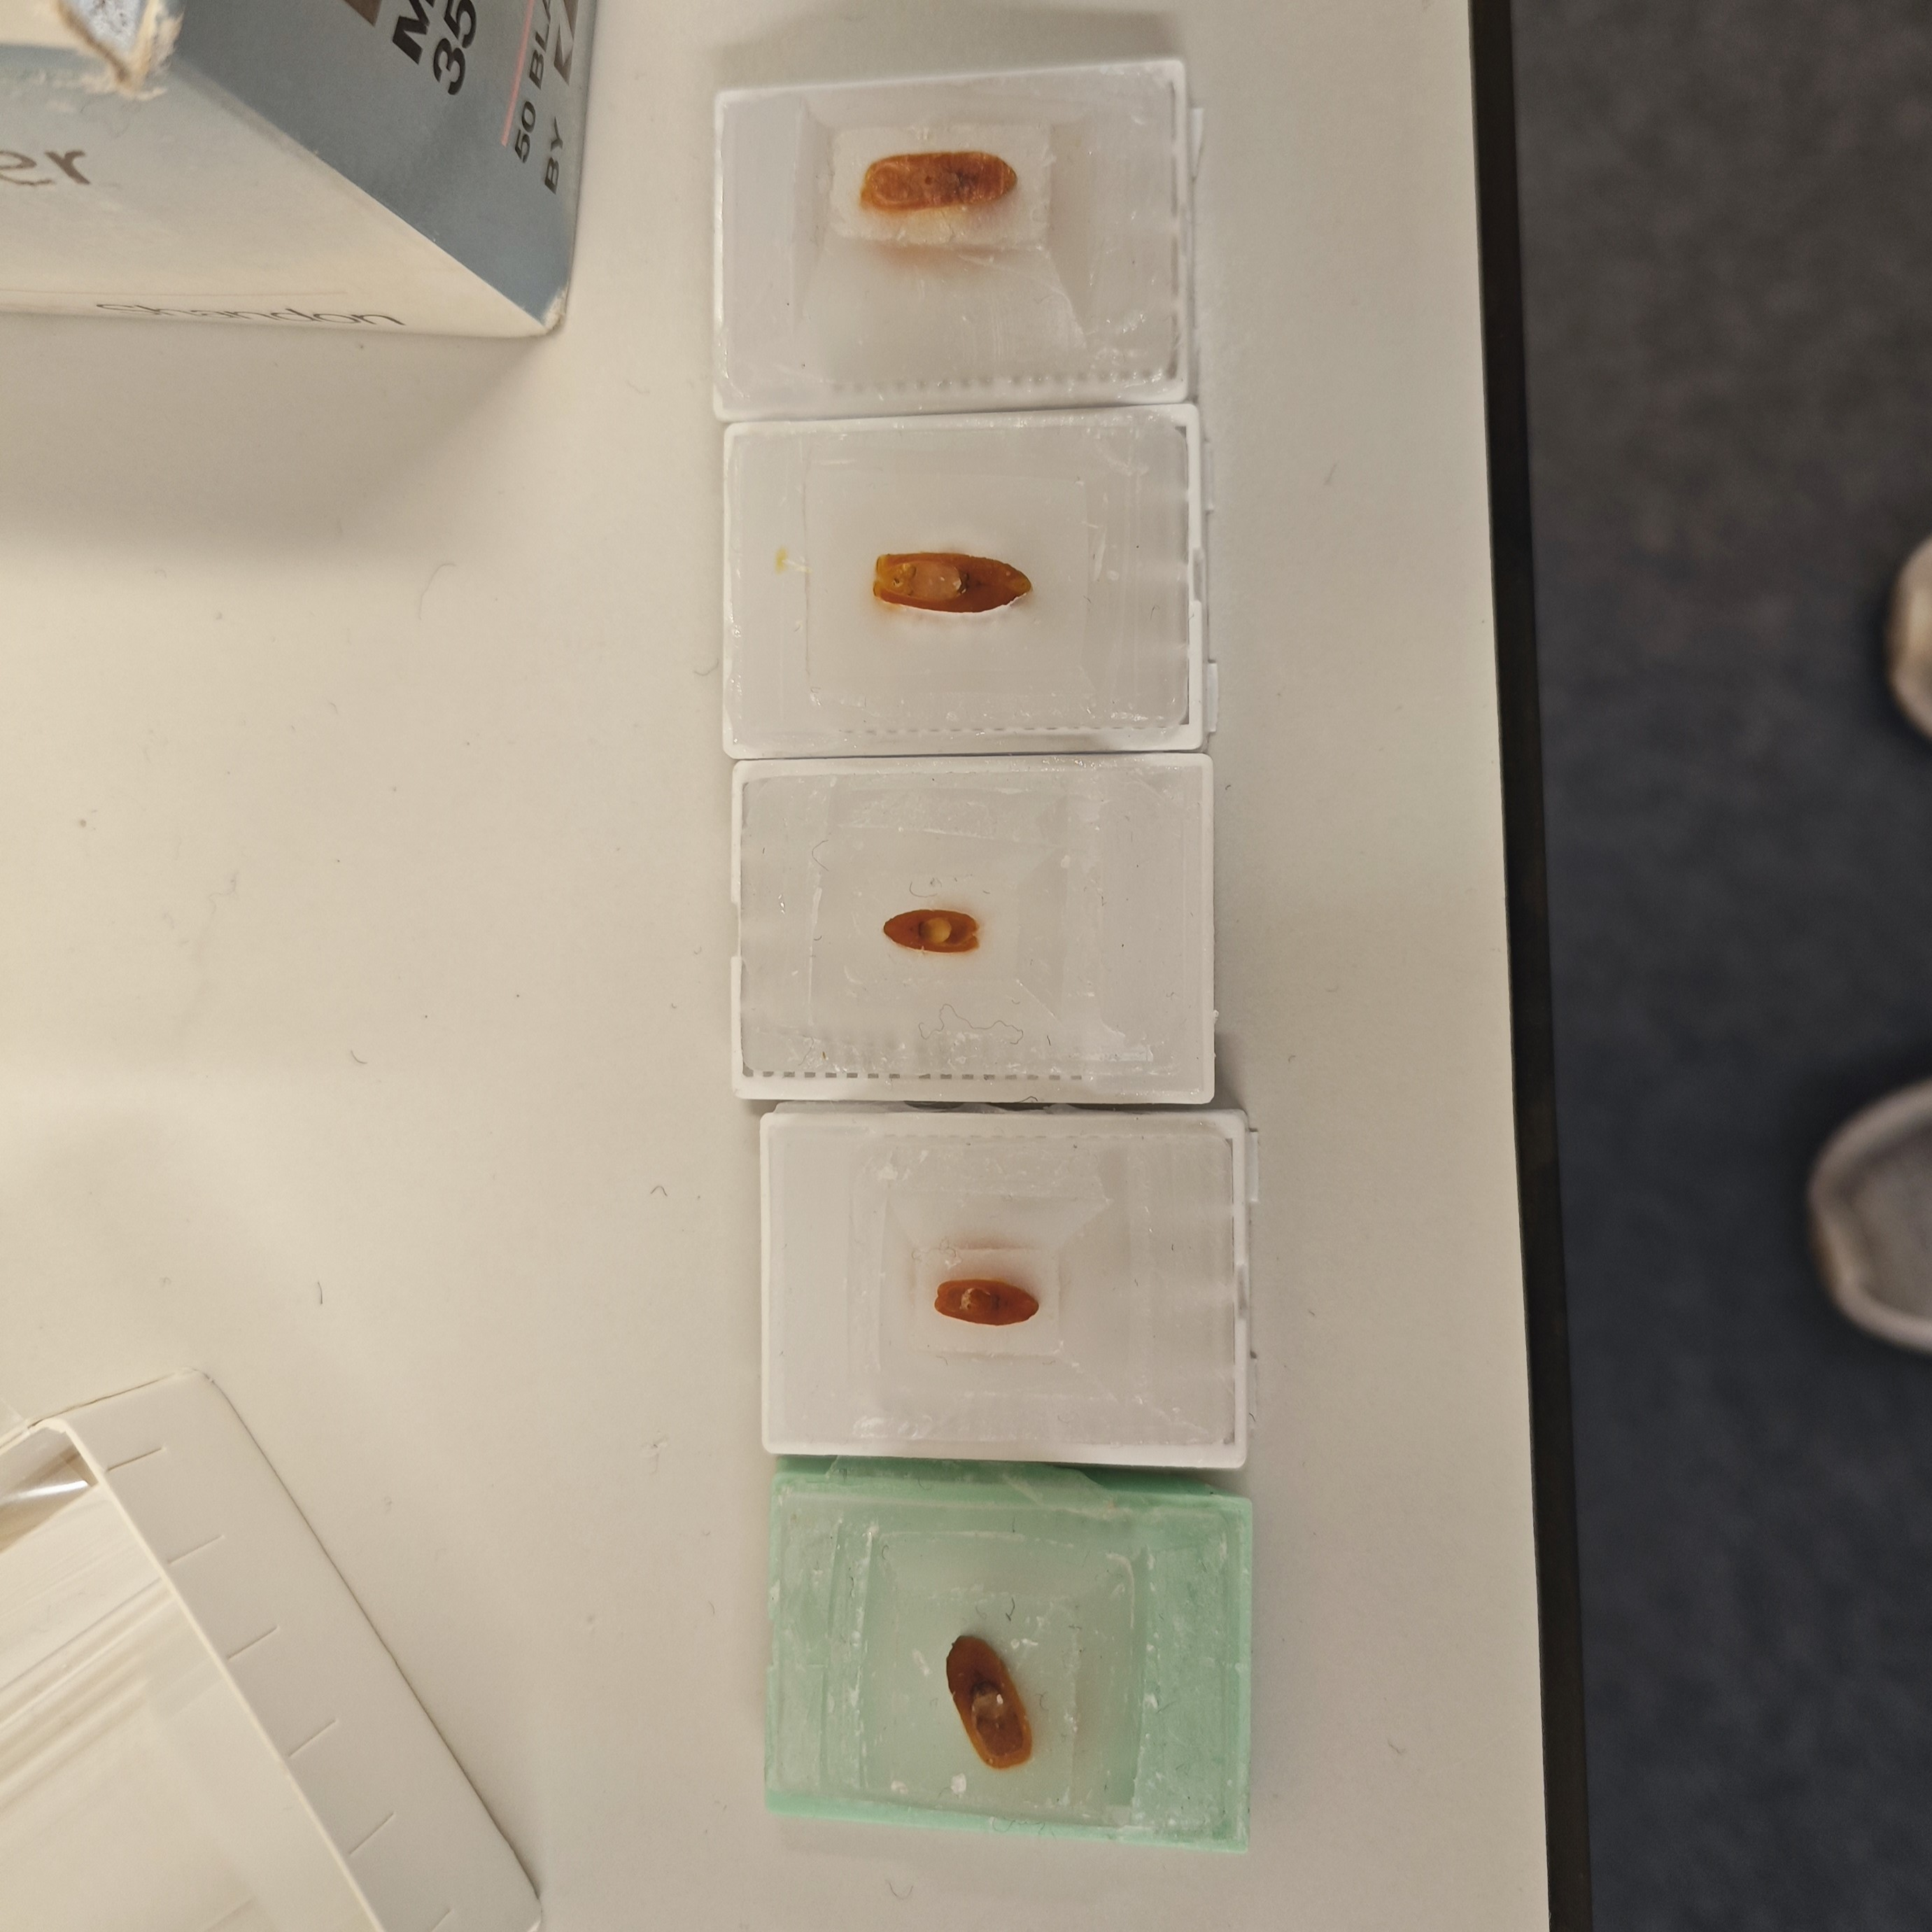
\includegraphics[width=\textwidth]{./fig/sample.jpg}
        \caption{Biological tissues}
        \label{label:sample}
    \end{minipage}
    \begin{minipage}{0.3\textwidth}
        \centering
        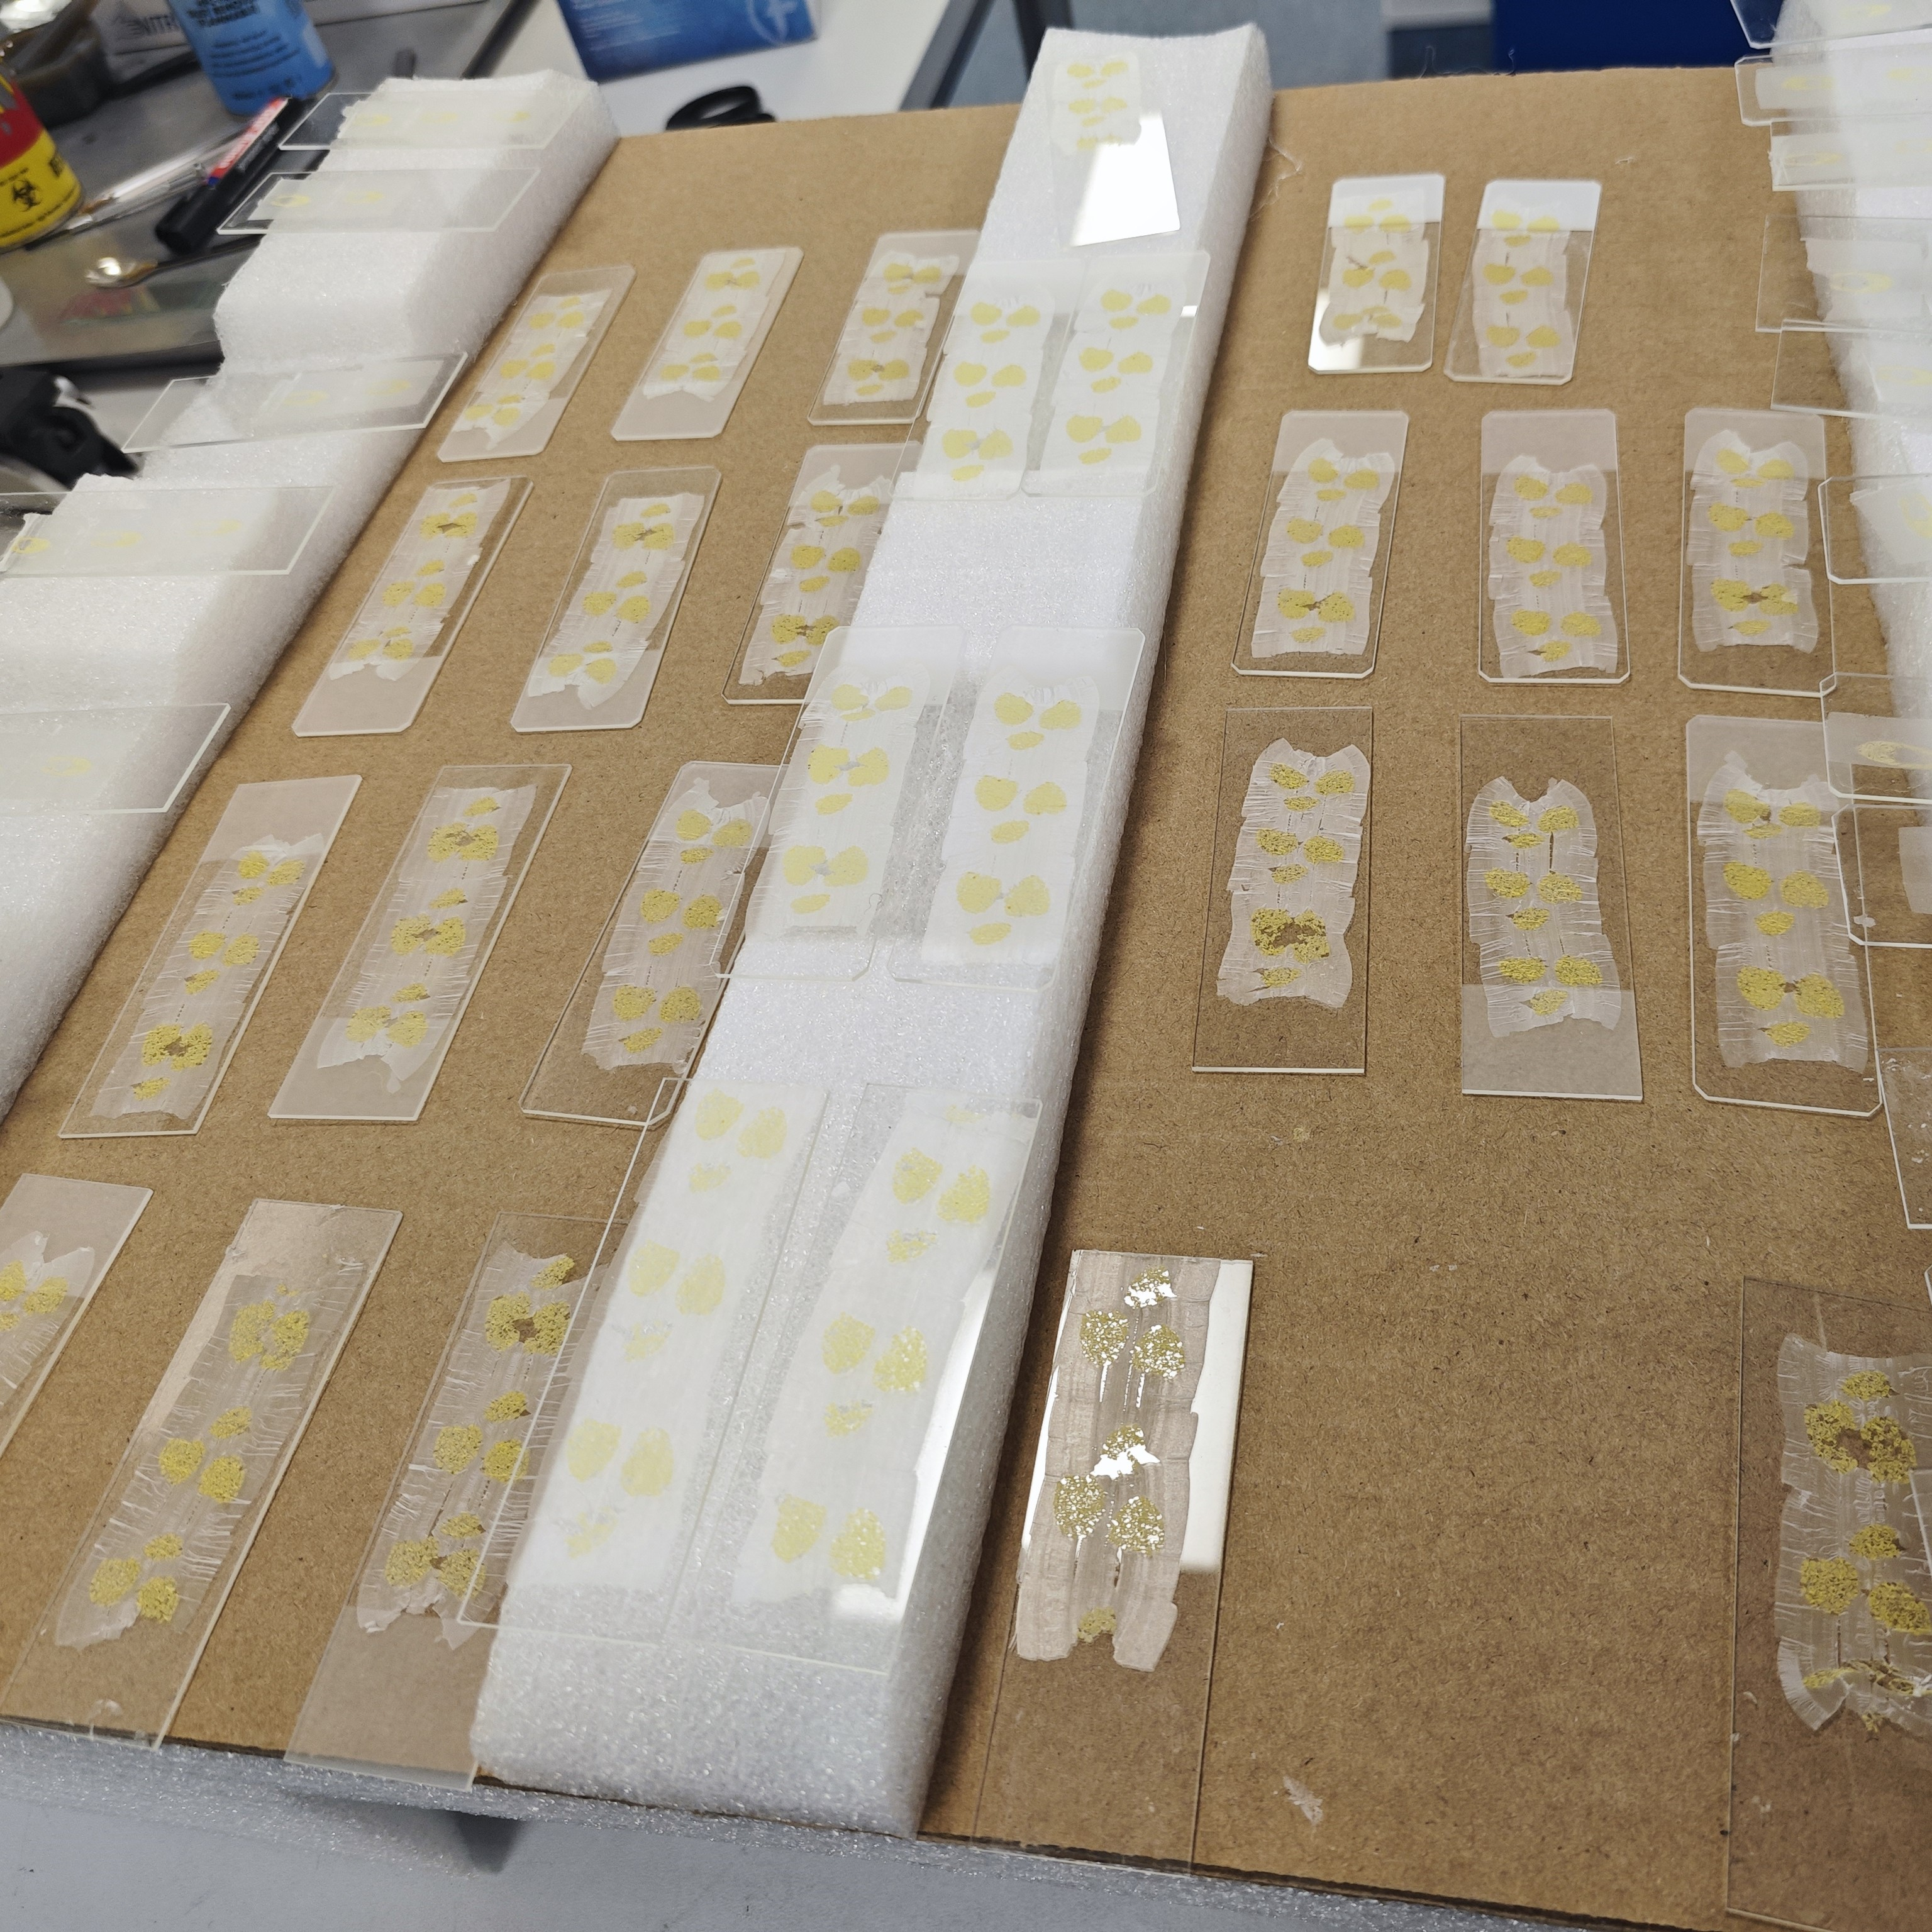
\includegraphics[width=\textwidth]{./fig/采集样本.jpg}
        \caption{Collecting samples}
        \label{fig:采集样本}
    \end{minipage}
    \begin{minipage}{0.35\textwidth}
        \centering
        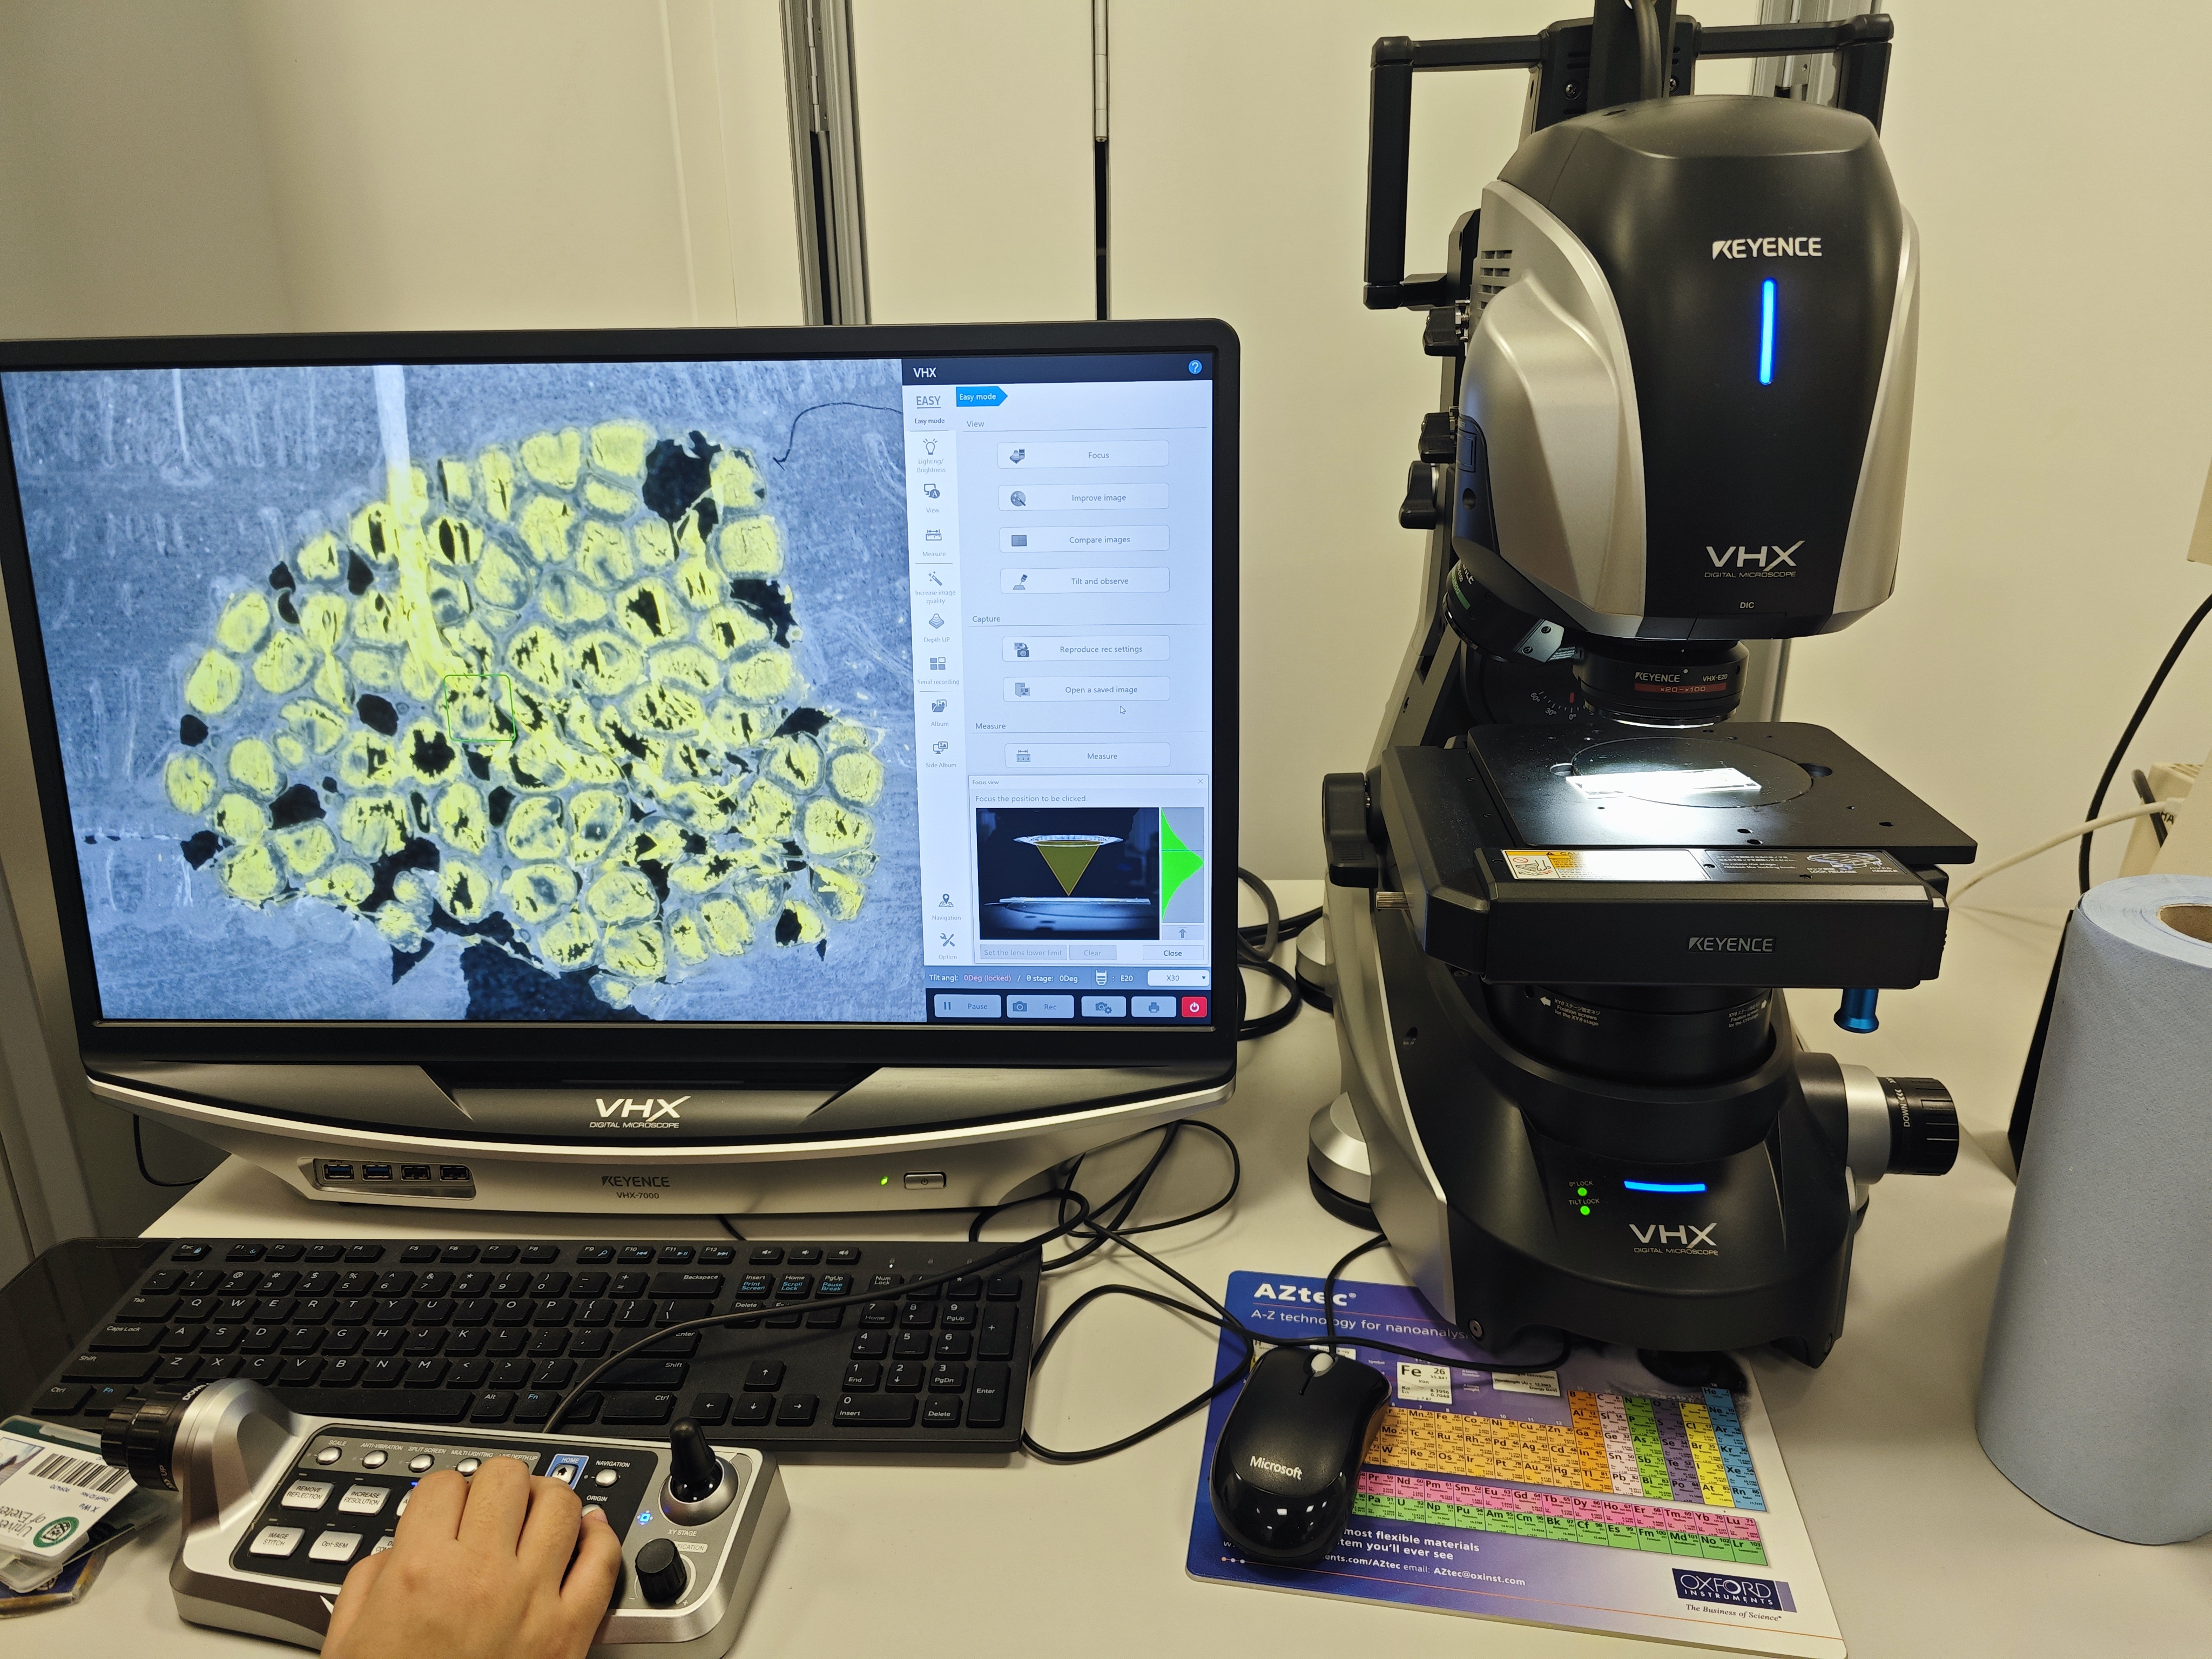
\includegraphics[width=\textwidth]{./fig/显微镜.jpg}
        \caption{Microscope}
        \label{fig:显微镜}
    \end{minipage}
\end{figure}


Based on this, several hundred images were obtained, each with a resolution of 2880*2160. 
% An example of the samples is shown in \autoref{fig:sample9.5}.


% \begin{figure}
%     \centering
%     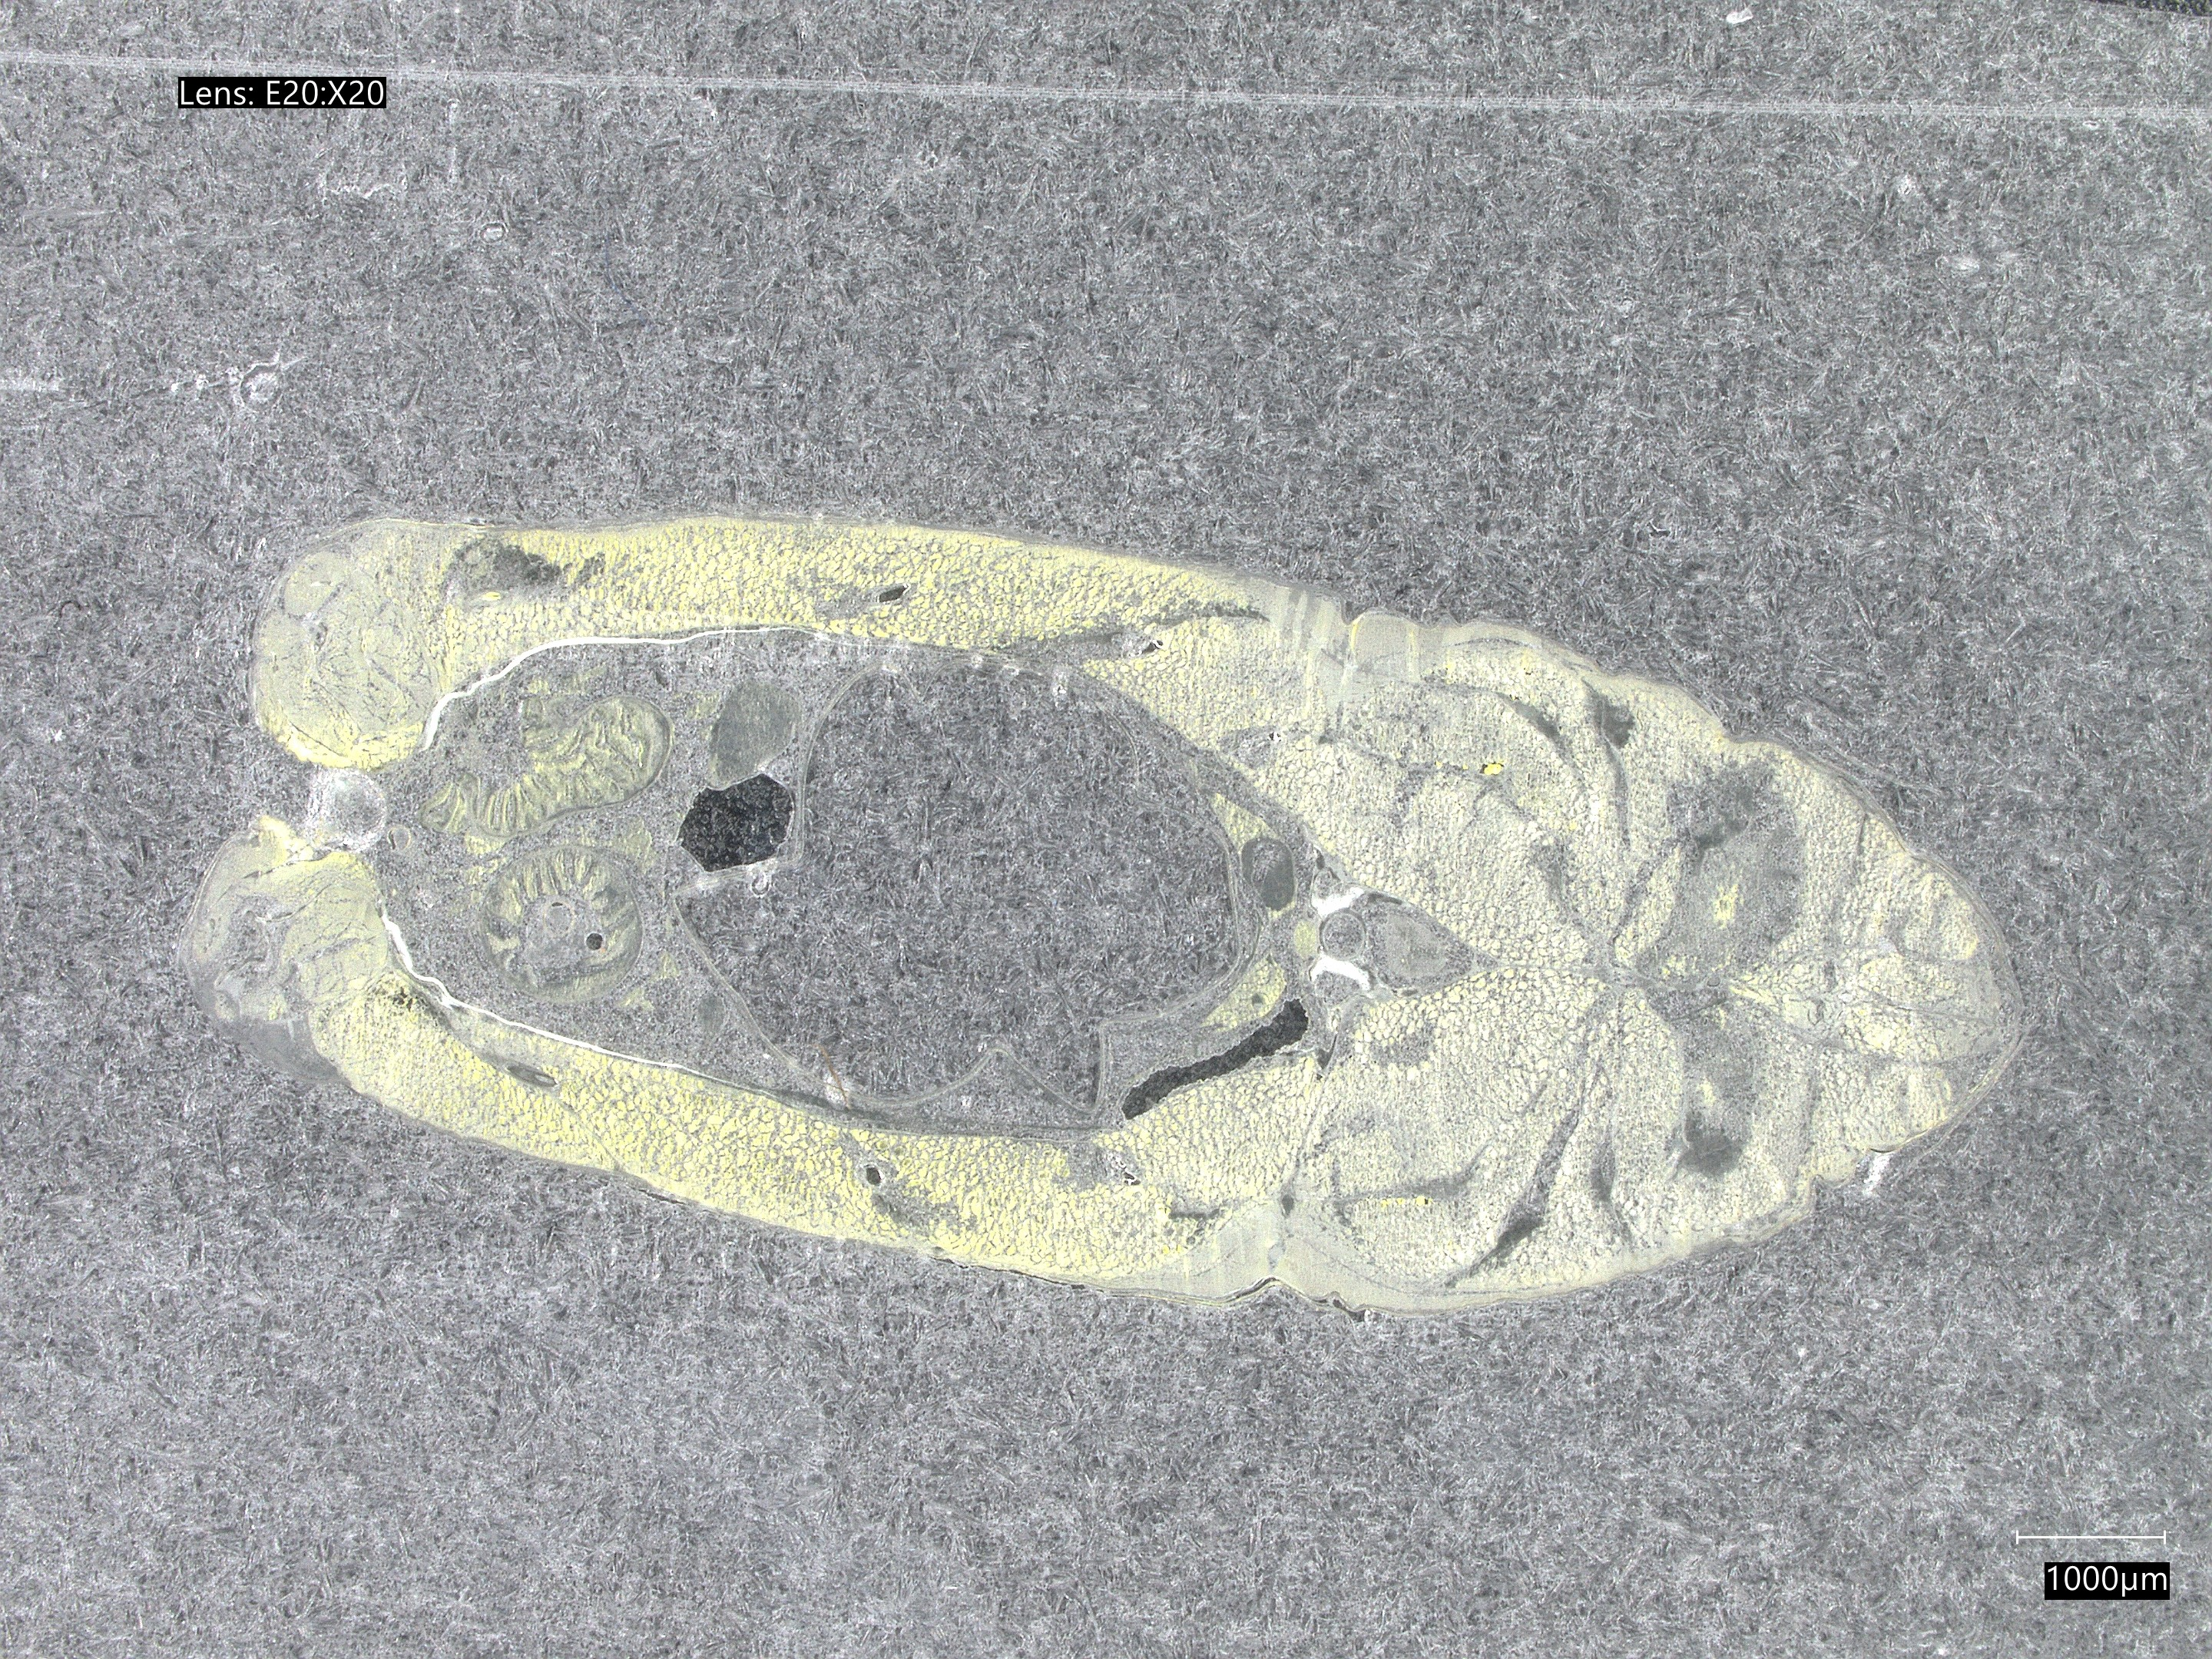
\includegraphics[width=0.8\textwidth]{./fig/sample9.5.jpg}
%     \caption{Sample with a cutting angle of 9.5 degrees}
%     \label{fig:sample9.5}
% \end{figure}


\subsection{Data Labeling}

For this experiment, the dataset is labeled based on the quality of the tissue sections. Overall, the quality of the biological tissues is categorized into two primary classes: normal and bad. Further analysis of the collected data revealed common flaws - the presence of vertical or horizontal white creases on the sections, which clearly indicate unusable slices. Given the distinct nature of these flaws, they are classified into two additional specific categories: \textbf{horizontal line}(\autoref{fig:horizental_line}) and \textbf{vertical line}(\autoref{fig:vertical_line}).

\begin{figure}[H]
    \centering
    \begin{minipage}{0.33\textwidth}
        \centering
        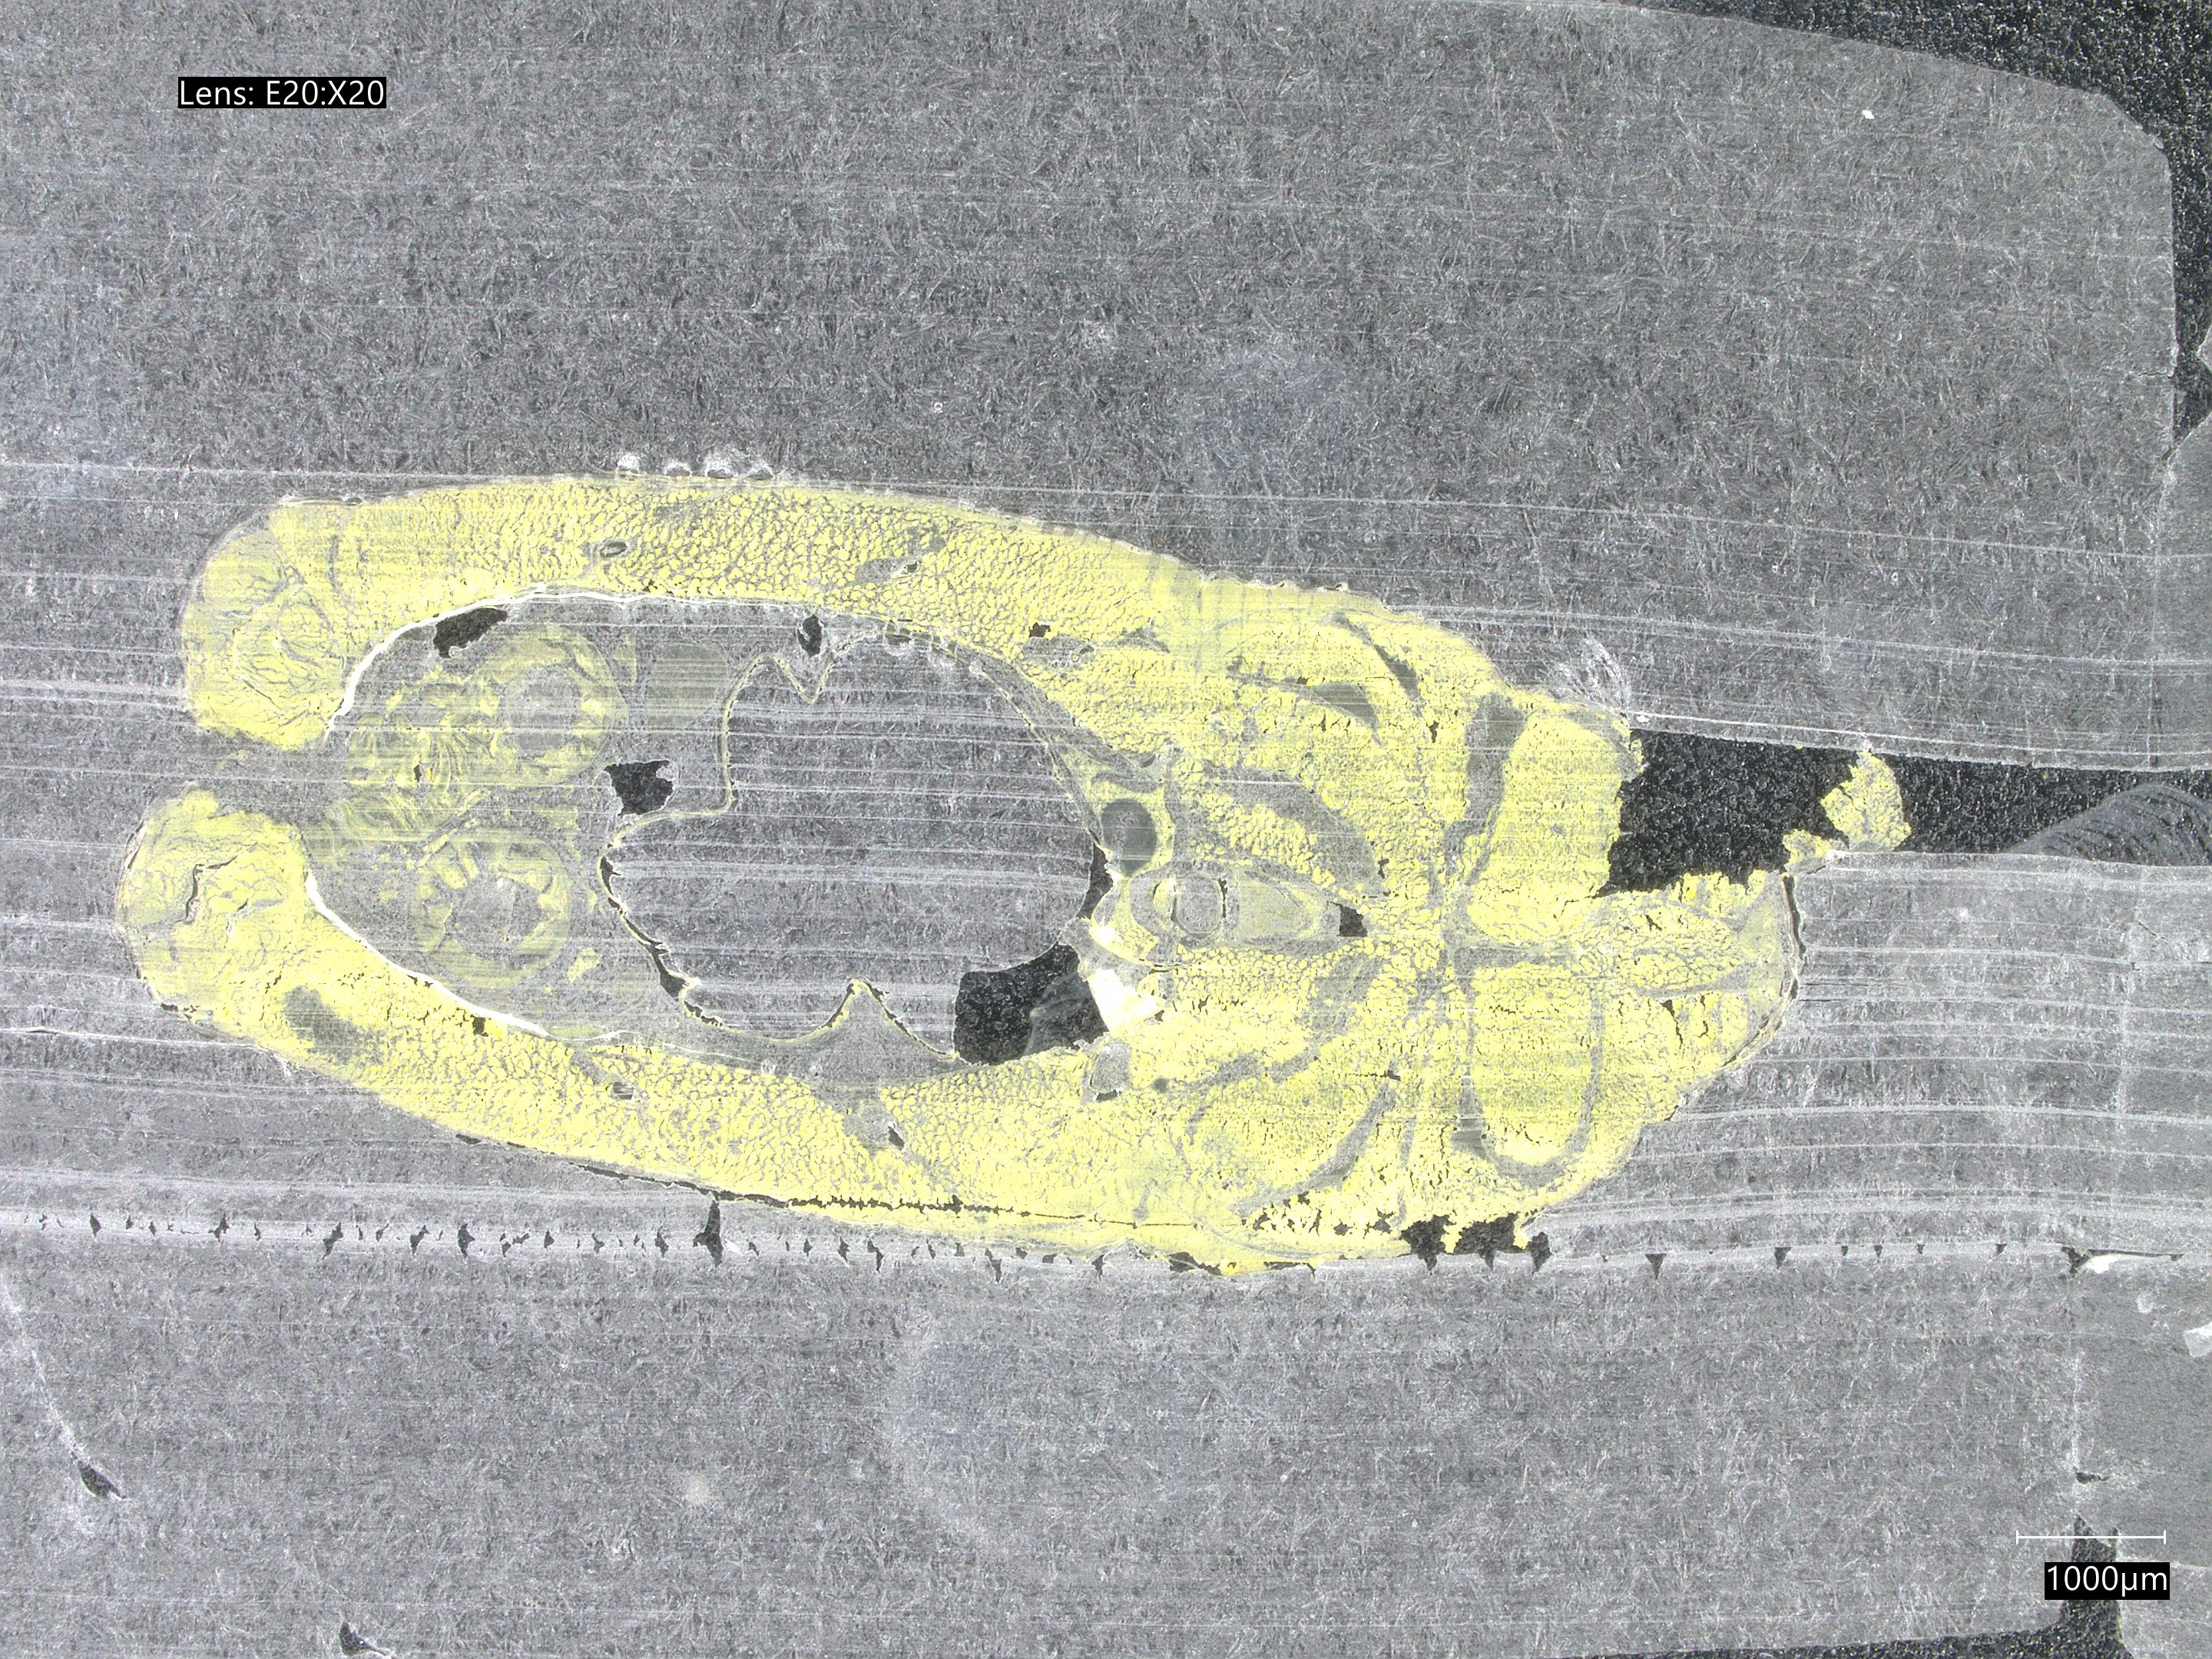
\includegraphics[width=\textwidth]{./fig/sample_1/horizental_line.jpg}
        \caption{horizental line}
        \label{fig:horizental_line}
    \end{minipage}
    \begin{minipage}{0.33\textwidth}
        \centering
        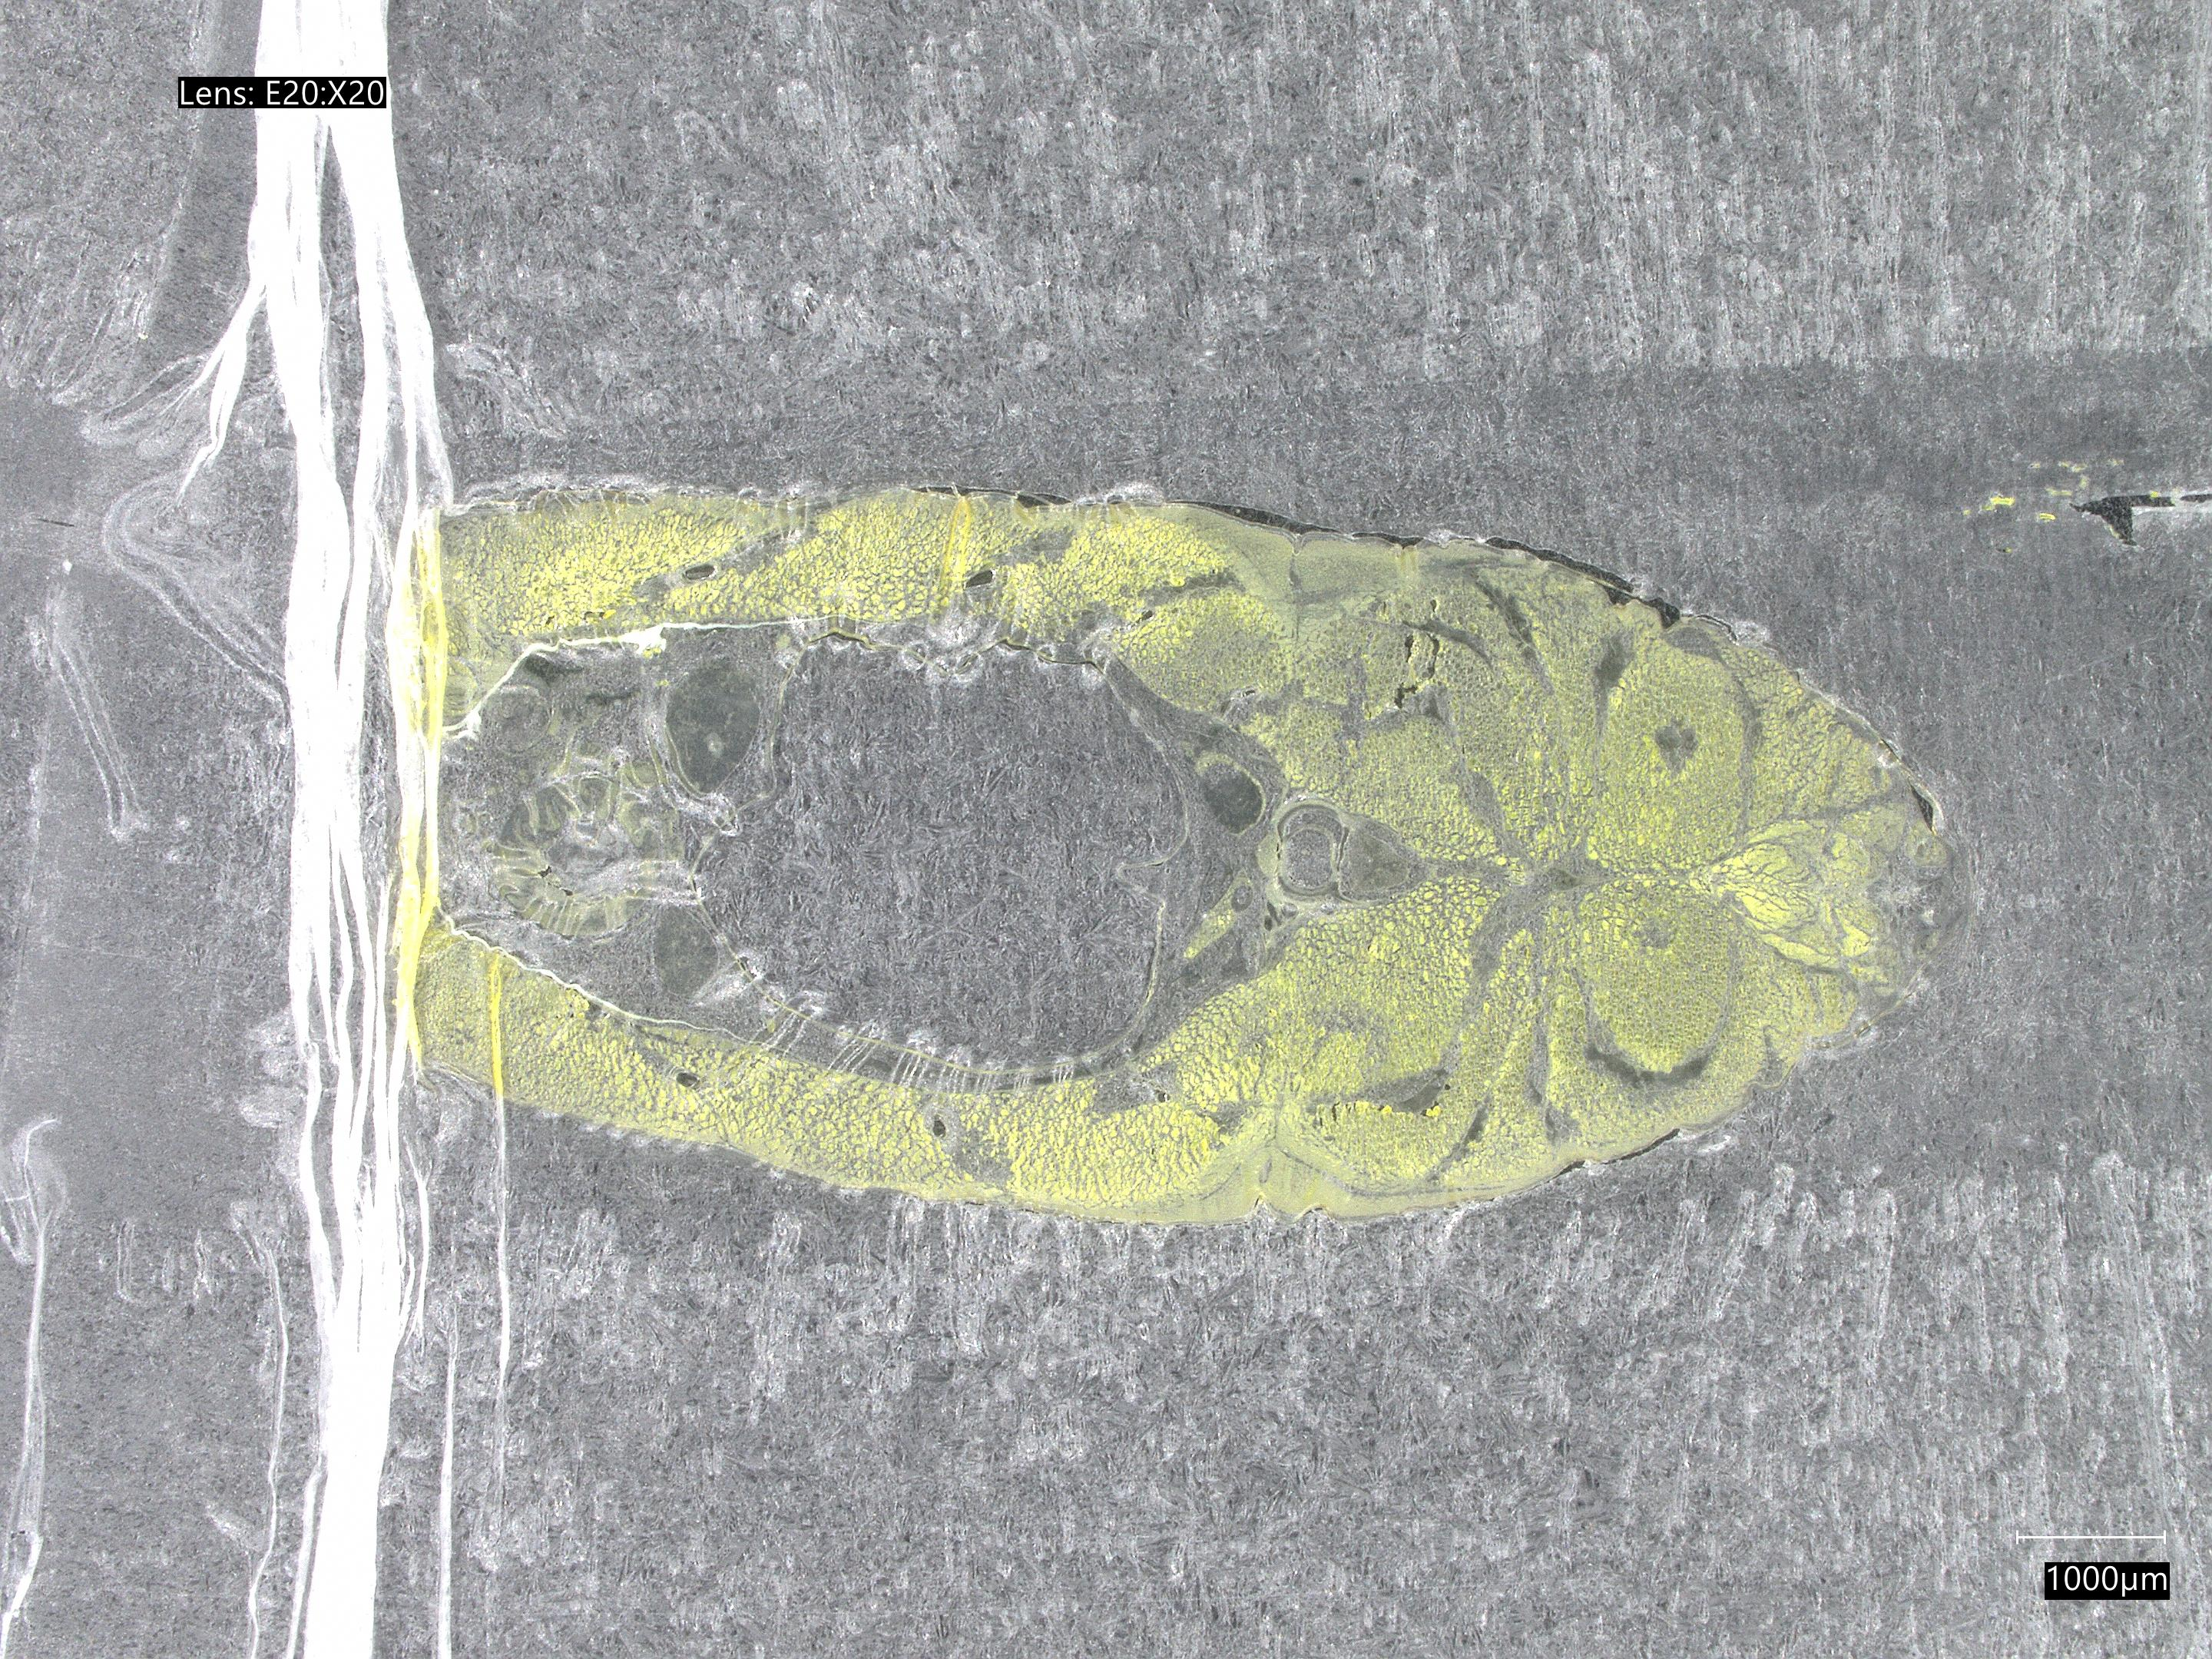
\includegraphics[width=\textwidth]{./fig/sample_1/vertical_line.jpg}
        \caption{vertical line}
        \label{fig:vertical_line}
    \end{minipage}
\end{figure}

Additionally, some images were noted to have a significant rotational angle at the time of sampling. These instances are categorized separately as \textbf{slope}(\autoref{fig:slope}). Finally, any images that do not fit into the aforementioned categories but still show irregularities(Excessive changes in brightness) are labeled as \textbf{other}(\autoref{fig:other}). 

\begin{figure}[H]
    \centering
    \begin{minipage}{0.32\textwidth}
        \centering
        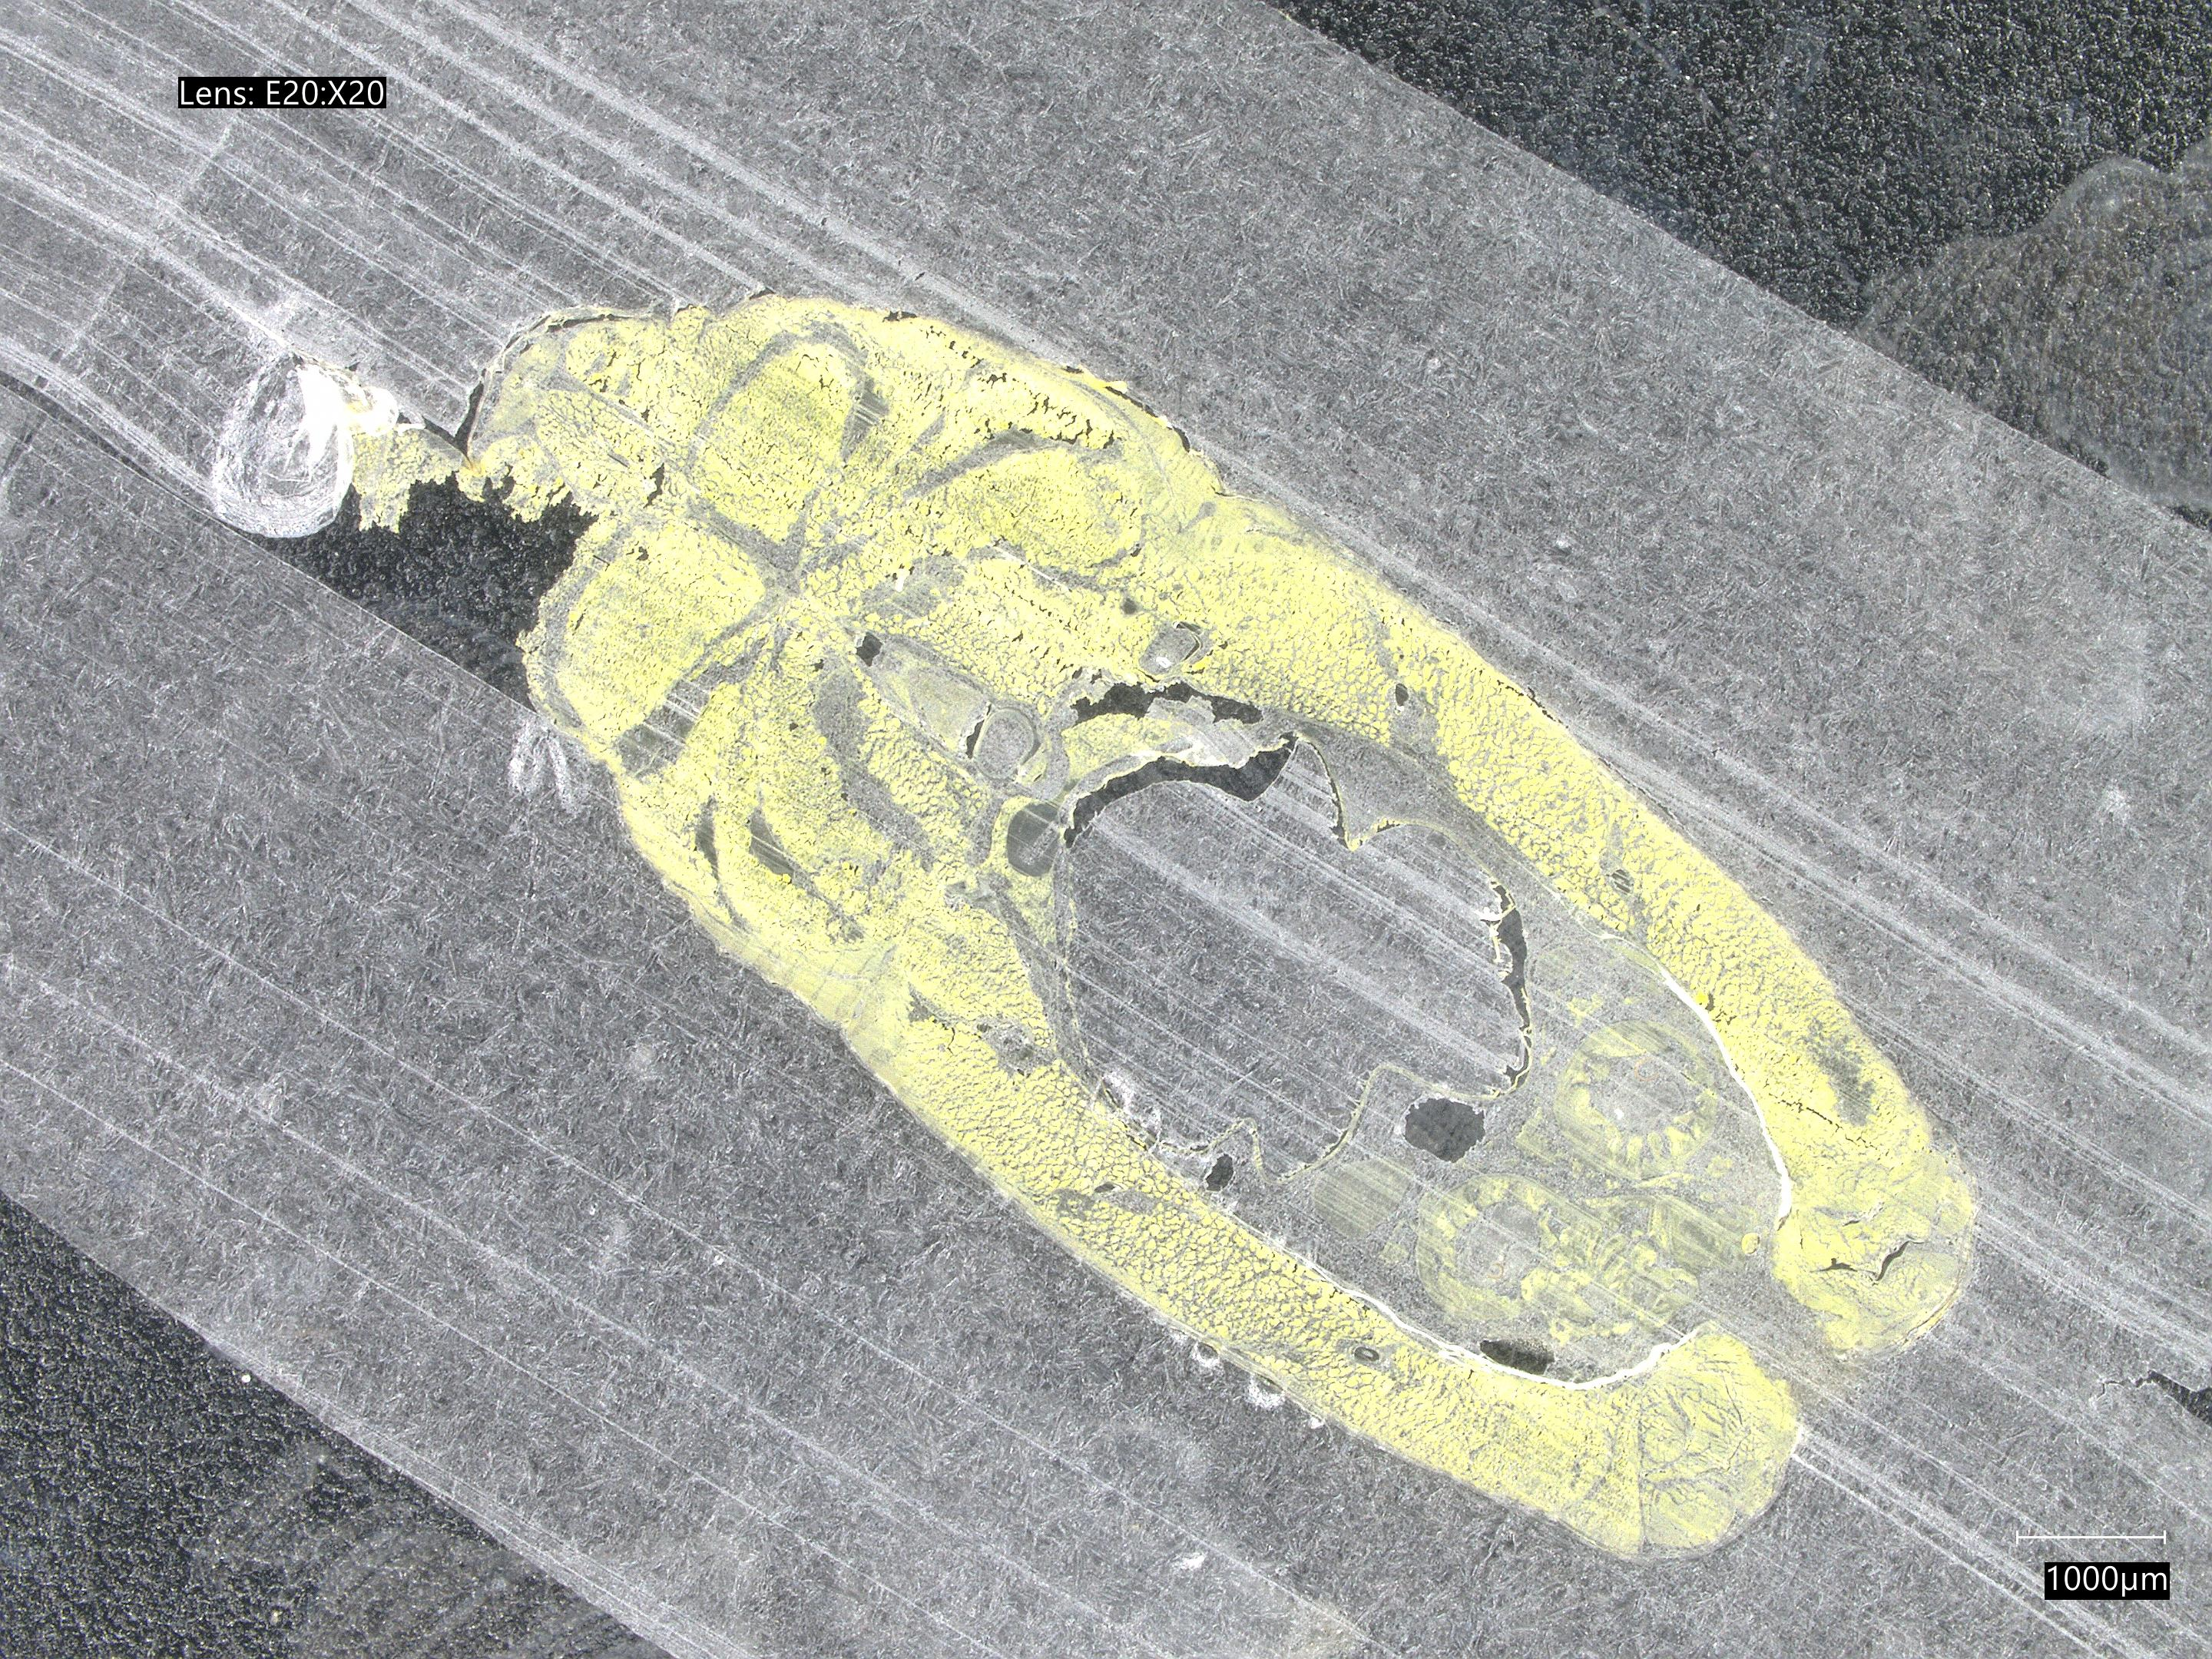
\includegraphics[width=\textwidth]{./fig/sample_1/slope.jpg}
        \caption{slope}
        \label{fig:slope}
    \end{minipage}
    \begin{minipage}{0.32\textwidth}
        \centering
        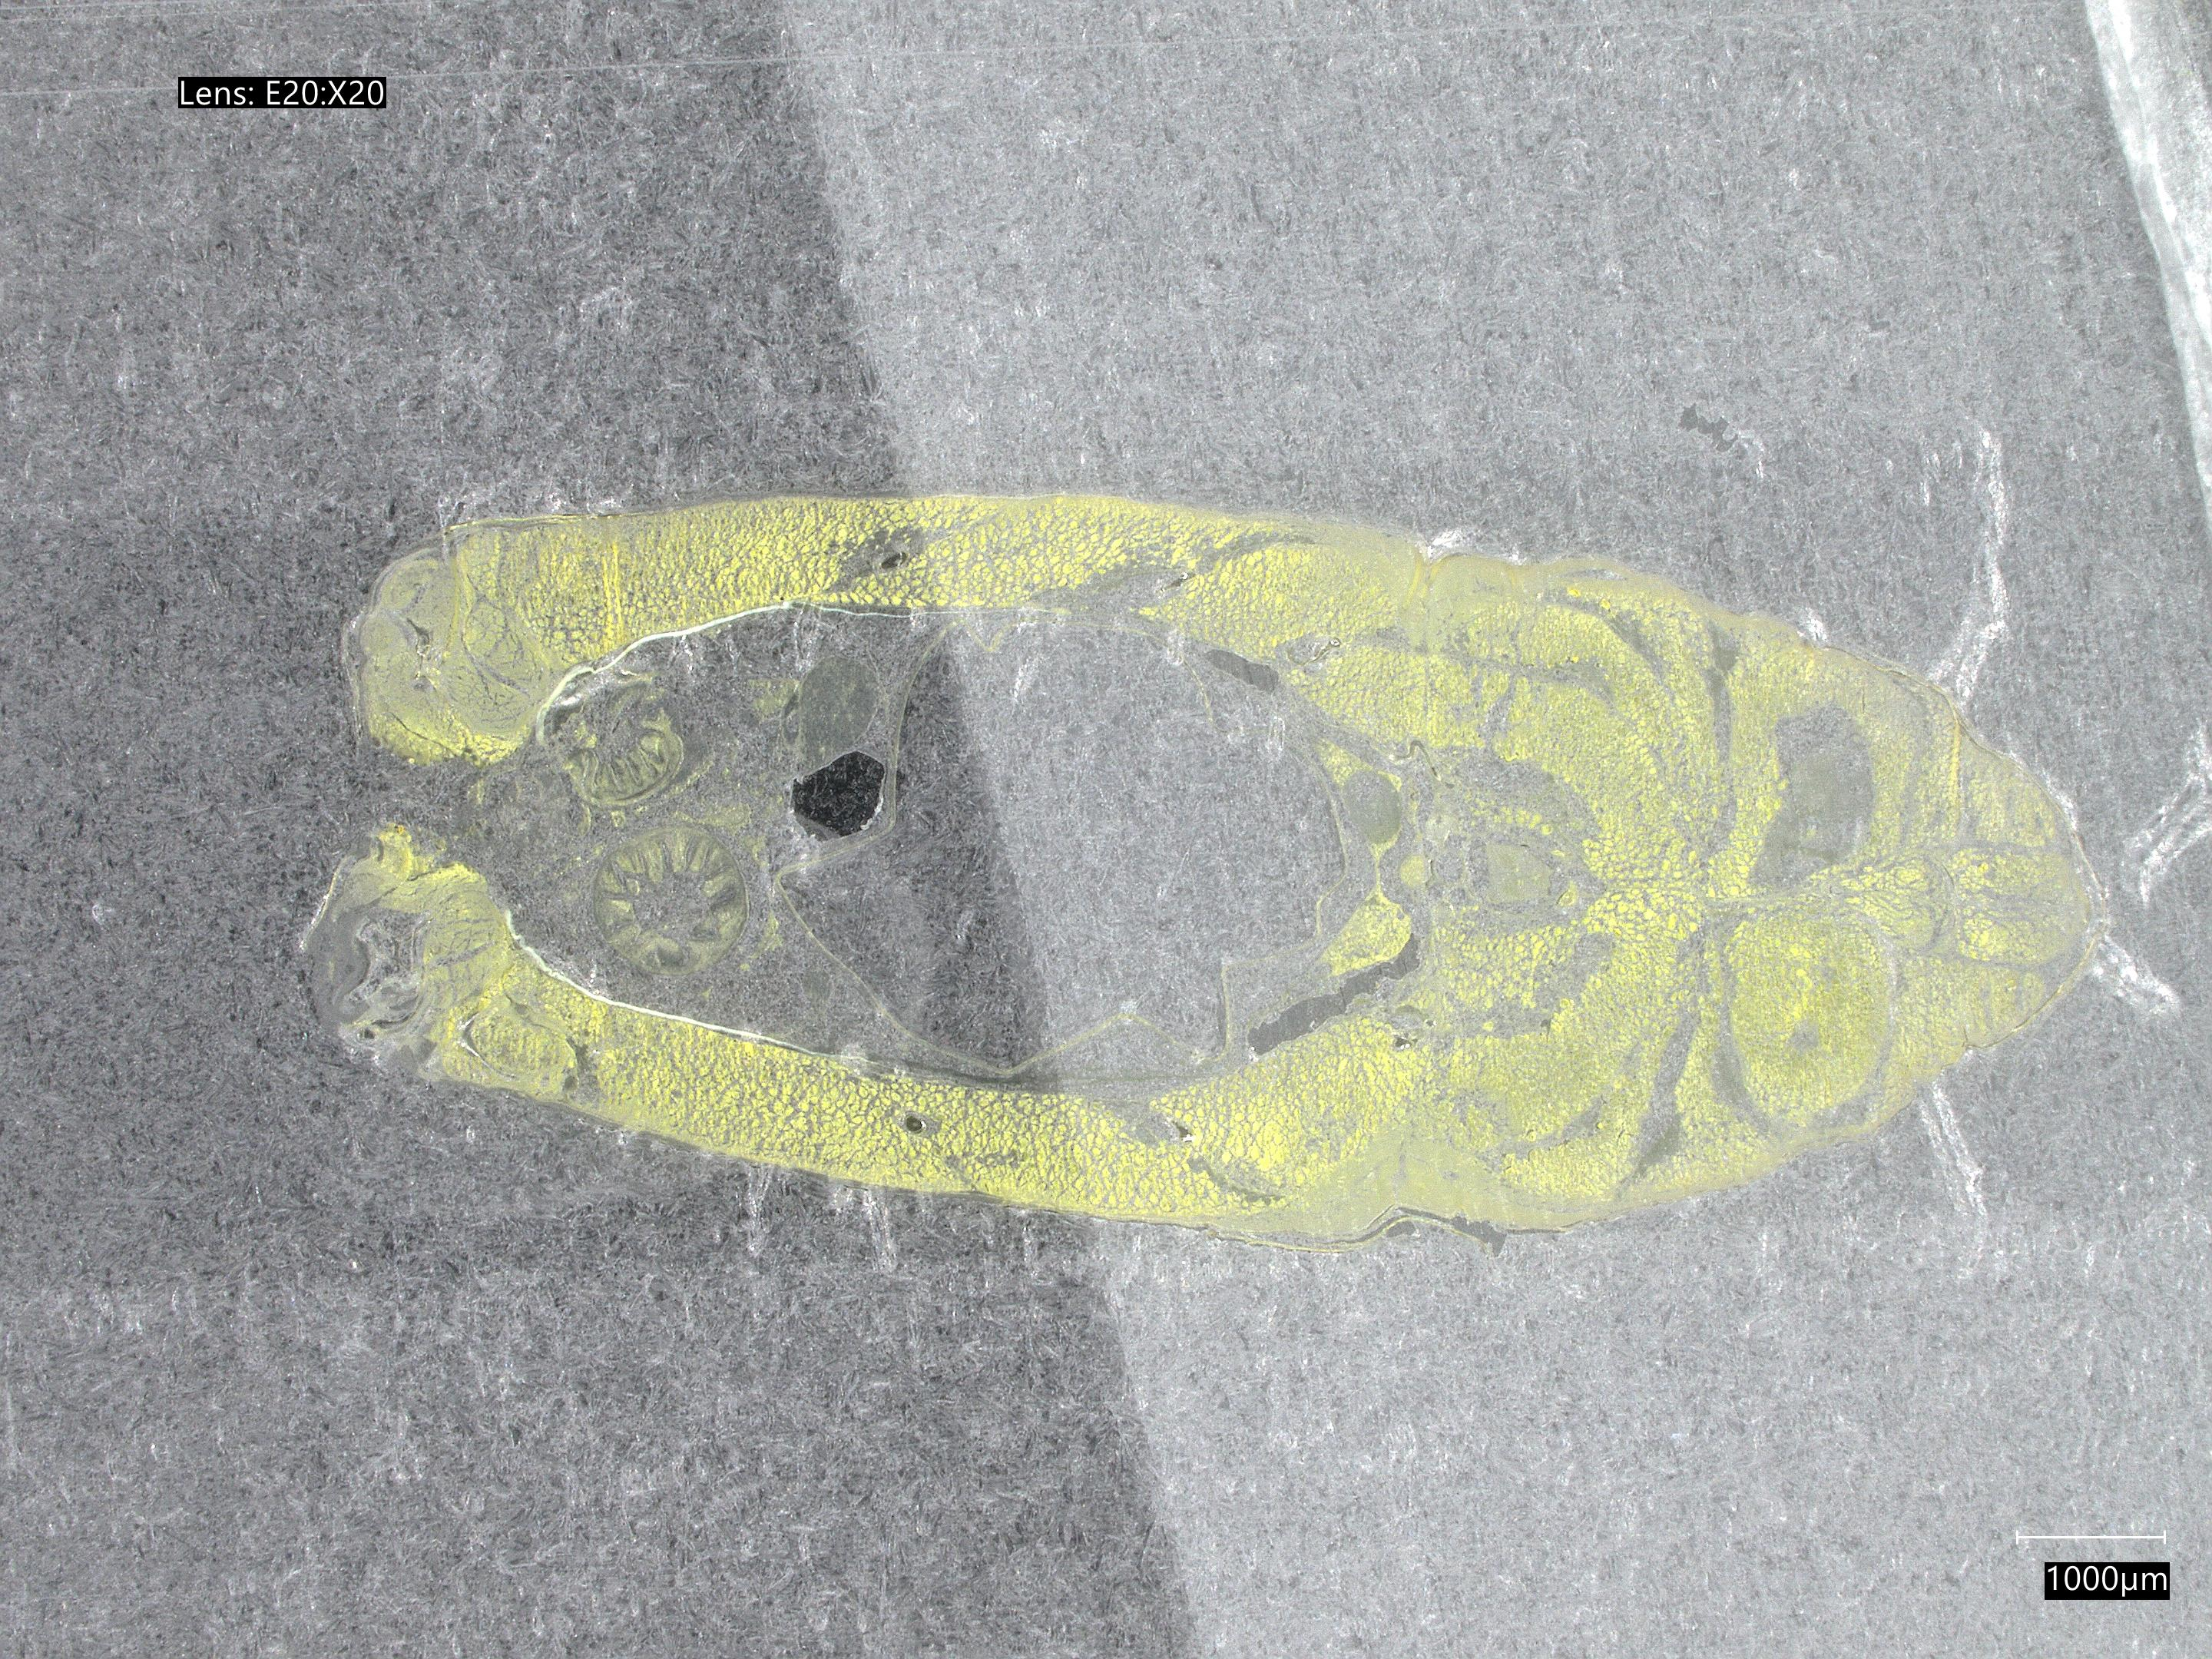
\includegraphics[width=\textwidth]{./fig/sample_1/other.jpg}
        \caption{other}
        \label{fig:other}
    \end{minipage}
    \begin{minipage}{0.32\textwidth}
        \centering
        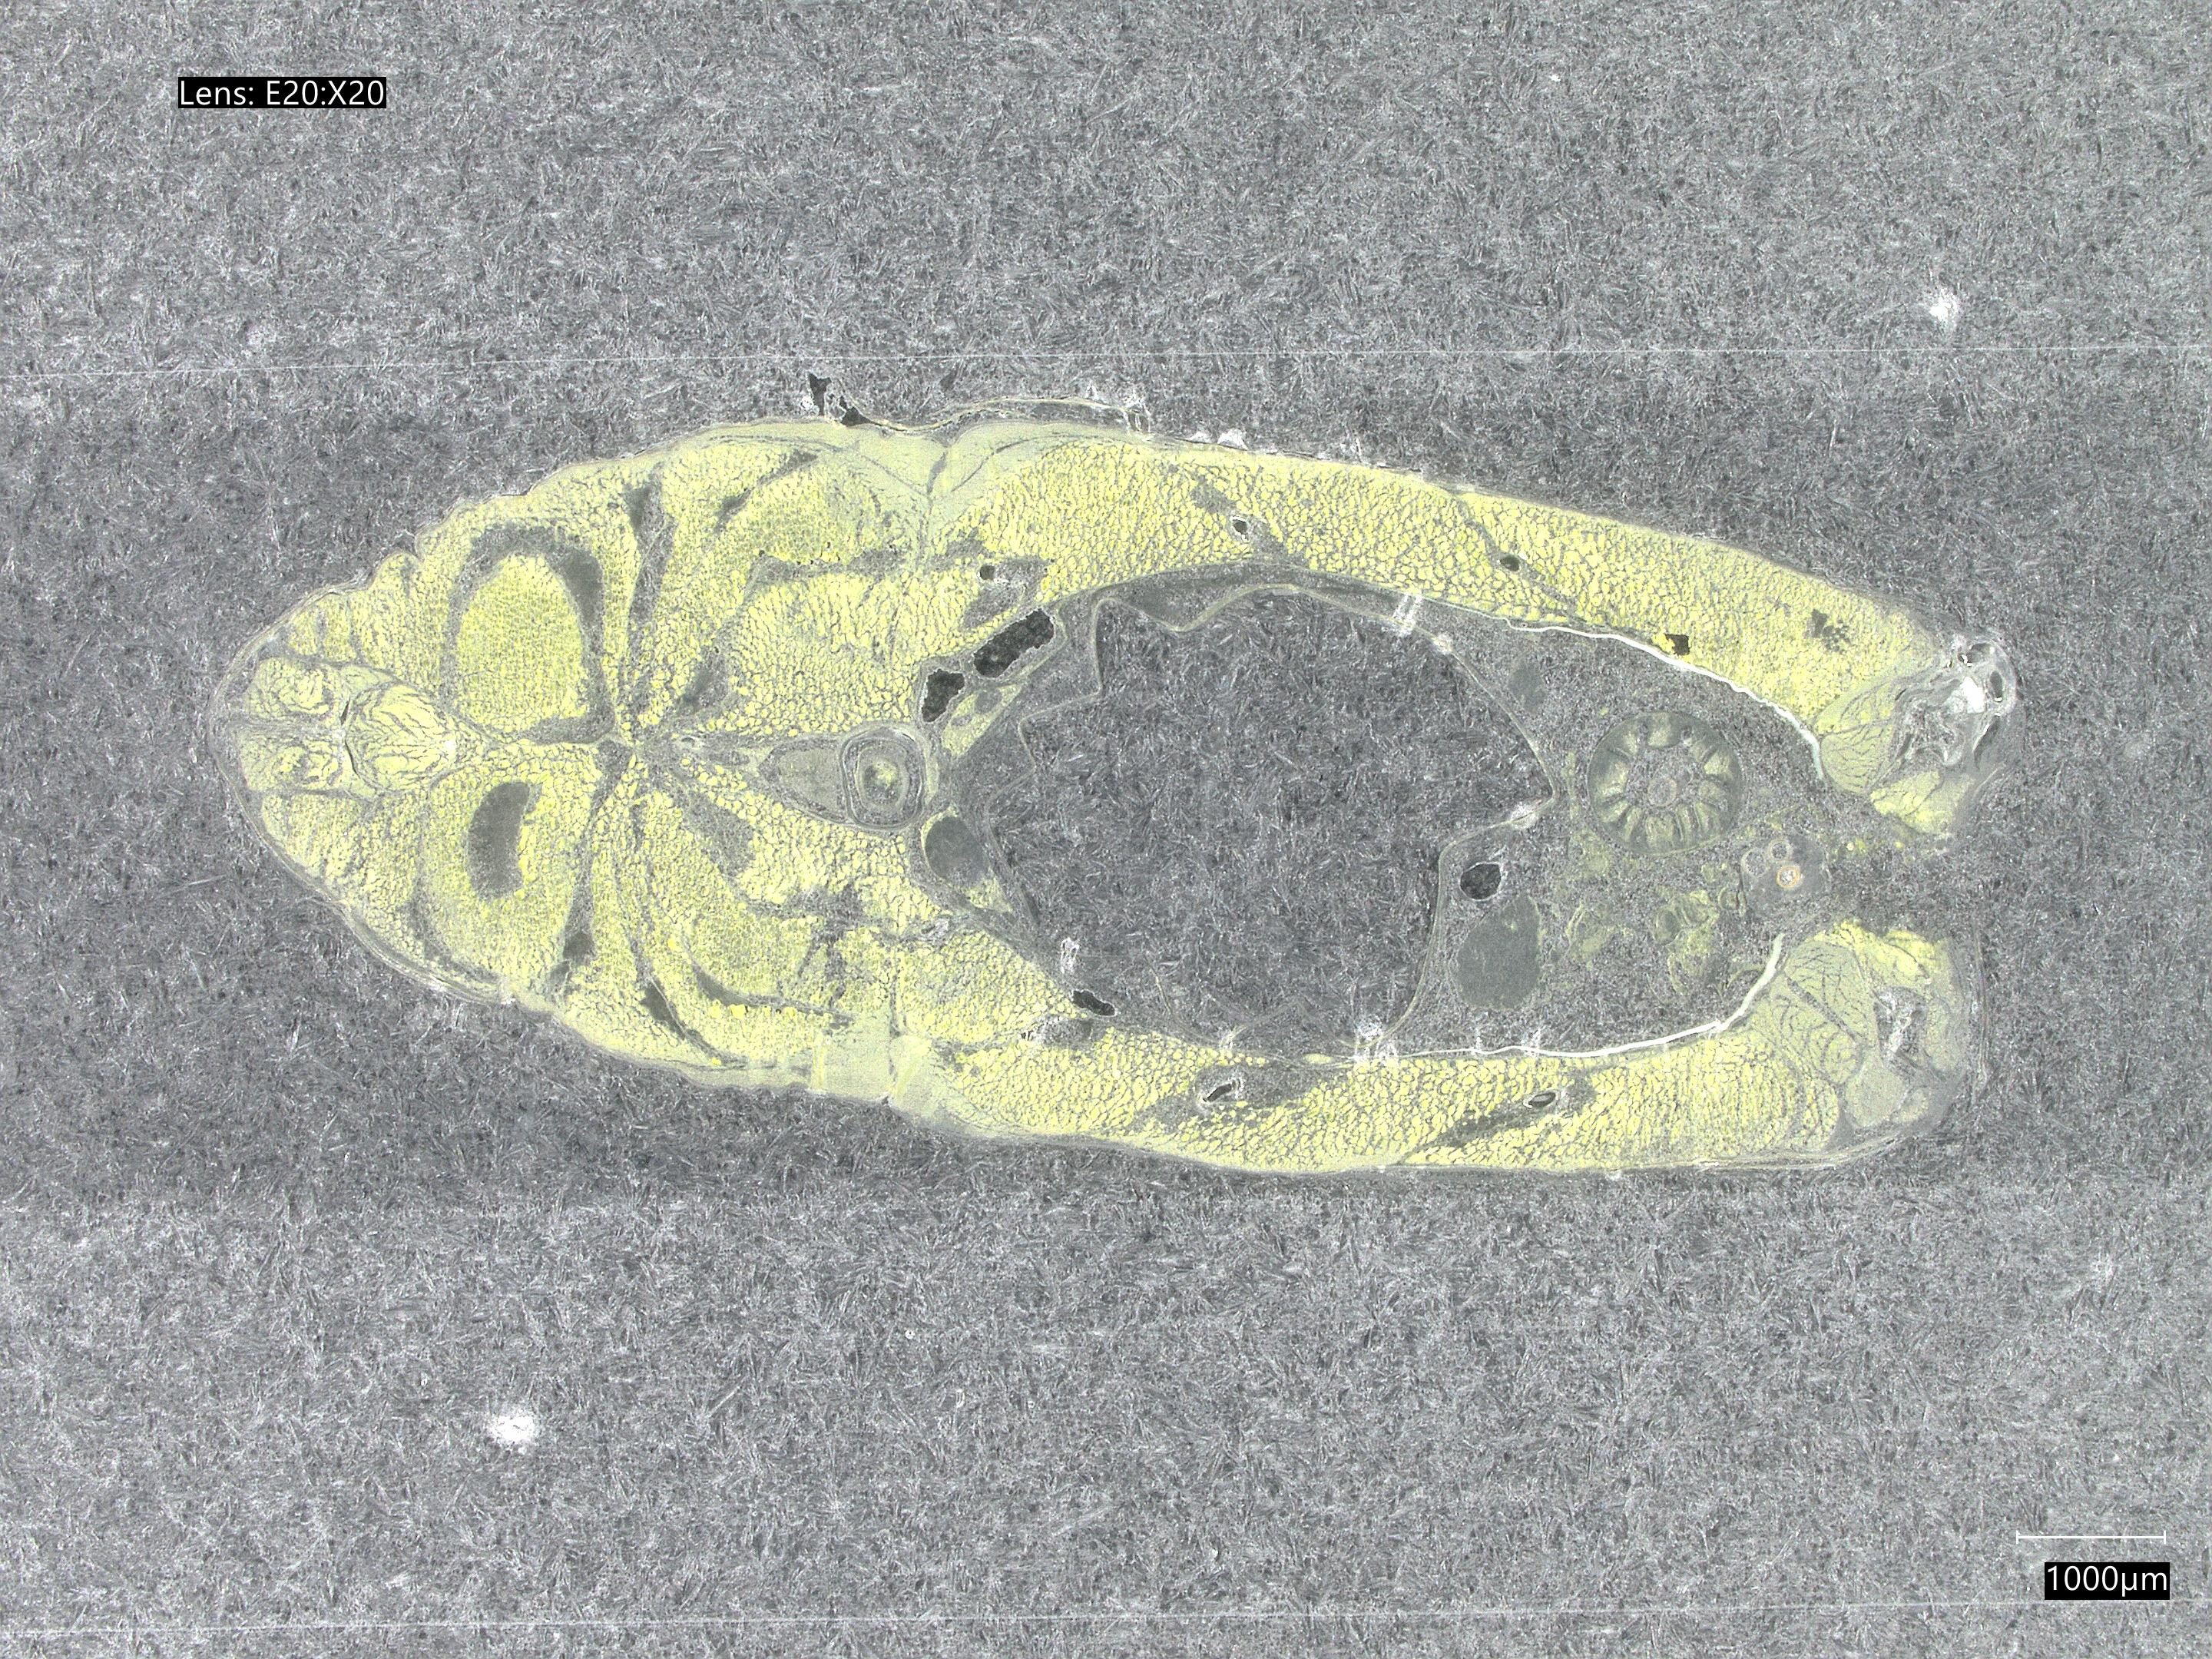
\includegraphics[width=\textwidth]{./fig/sample_1/normal.jpg}
        \caption{normal}
        \label{fig:normal}
    \end{minipage}
\end{figure}

An example of a normal slice that meets observational requirements is shown in \autoref{fig:normal}.


For each image, we need to label it as one of the above five categories. This will serve as our dataset for training the model.


\FloatBarrier

\subsection{Model 1: Original Images with a Simple CNN Network}

For a new dataset, where the appropriate complexity of the model for the given image complexity is uncertain, a basic CNN architecture is initially employed to gauge the characteristics of the dataset and the complexity of the images.

\begin{table}[H]
\centering
\caption{Configuration of the simple CNN model}
\begin{tabular}{ccccc}
    \toprule
    \textbf{Layer Type} & \textbf{Configuration 1a} & \textbf{Configuration 1b} & \textbf{Configuration 1c} \\
    \midrule
    Input Layer & - & - & - \\
    Conv Layer 1 & Conv3-32 (relu) & Conv3-16 (relu) & Conv3-32 (relu) \\
    Pooling Layer 1 & MaxPooling & MaxPooling& MaxPooling \\
    Conv Layer 2 & Conv3-32 (relu) & Conv3-32 (relu) & Conv3-32 (relu) \\
    Pooling Layer 2 & MaxPooling & MaxPooling& MaxPooling \\
    Conv Layer 3 & Conv3-32 (relu) & Conv3-64 (relu) & Conv3-32 (relu) \\
    Pooling Layer 3 & MaxPooling & MaxPooling& MaxPooling \\
    Flattening Layer & Flatten() & Flatten() & Flatten() \\
    FC(Full connect) & Dense(128, relu) & Dense(128, relu) & Dense(256, relu) \\
    Output Layer & - & - & - \\
    \bottomrule
\end{tabular}
\label{tab:cnn_simple_configuration}
\end{table}

The configurations of the simple CNN models used are outlined in \autoref{tab:cnn_simple_configuration}. These initial models, labeled as Configuration 1a, 1b, and 1c, vary in terms of the number of neurons in the convolutional layers and the size of the neurons in the fully connected layers. Configuration 1a and 1b differ by the number of neurons in the convolutional layers, whereas Configuration 1c differs from Configuration 1a in the size of the neurons in the fully connected layer.

The preprocessing steps involve splitting the dataset into training (80\%) and testing (20\%) sets. In the input layer, the image dimensions are halved (from 2880x2160 to 1440x1080), and the data is normalized.

During training, the Adam optimizer and cross-entropy loss function are used, with early stopping implemented to avoid overfitting.

The graphs below display the accuracy and loss of Models 1a, 1b, and 1c over the training epochs.

\begin{figure}[H]
    \centering
    \begin{minipage}{0.49\textwidth}
        \centering
        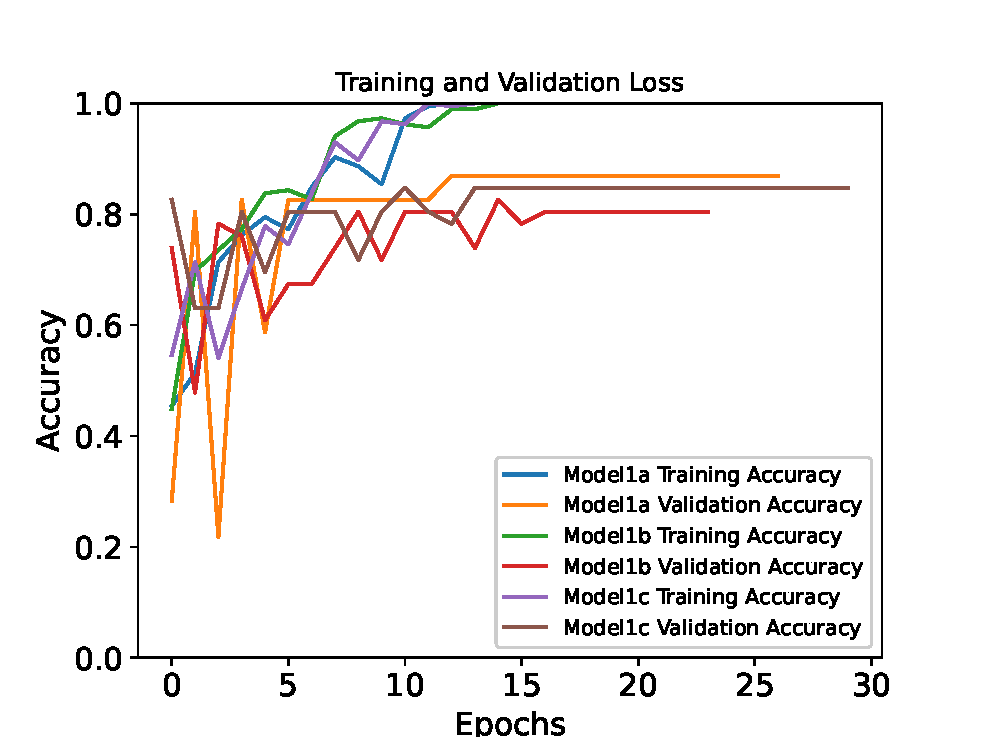
\includegraphics[width=\textwidth]{./fig/model1/accuracy11.eps}
        \caption{Accuracy of Model 1}
        \label{fig:model11_acc}
    \end{minipage}
    \begin{minipage}{0.49\textwidth}
        \centering
        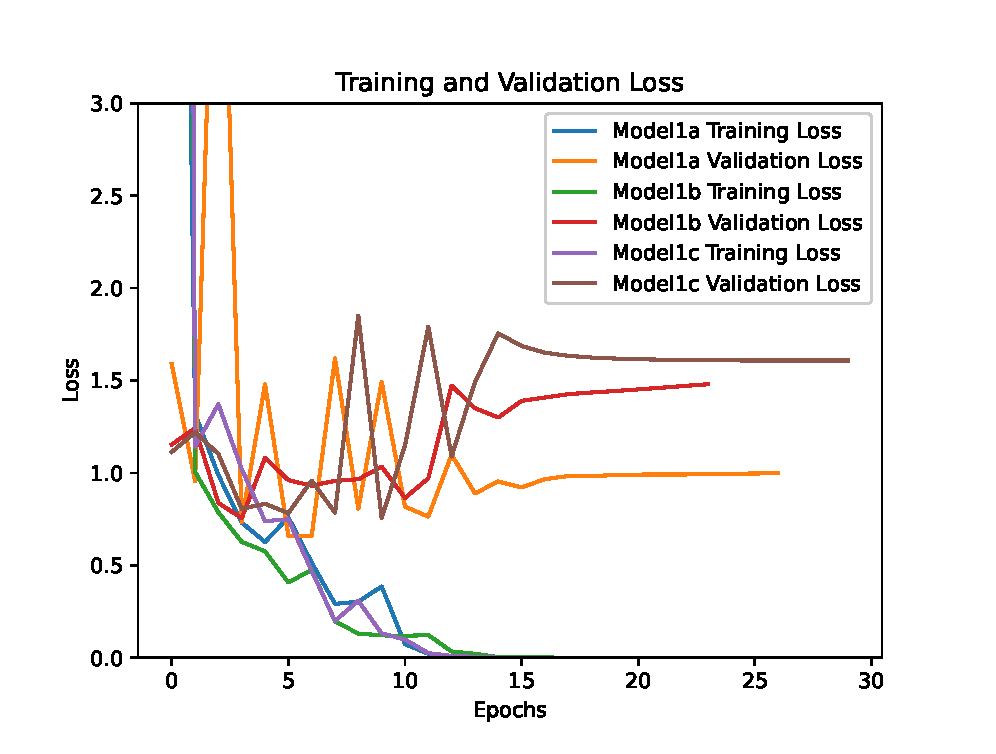
\includegraphics[width=\textwidth]{./fig/model1/loss11.eps}
        \caption{Loss of Model 1}
        \label{fig:model11_loss}
    \end{minipage}
\end{figure}


From the charts, it is observed that Models 1a, 1b, and 1c exhibit a gradual increase in training accuracy, stabilizing over time, while training losses decrease, approaching zero. This indicates that the models are learning from the training data relatively well. However, for the validation set, the accuracy of all three models stabilizes within the range of 80\% to 85\%, and the validation loss is comparatively high in some cases, especially with Model 1a, where it approaches 2.5 and shows significant fluctuations. This suggests a degree of overfitting, where the models perform better on the training data than on unseen data. Notably, Model 1c shows the best performance in terms of validation loss, indicating that its structure or parameter adjustments may be more effective at improving generalization.

The likely cause of overfitting here could be the insufficient complexity of the models relative to the complexity of the dataset, indicating that the models may not be effectively extracting features from the data. Although the models achieve high accuracy and low losses on the training set, their generalization capabilities on the validation set need enhancement.

To improve model accuracy, considering preprocessing of the images and assisting the model with feature extraction manually might be beneficial, helping the model better generalize to new data.

\FloatBarrier


\subsection{Image Preprocessing Improvement}

In cases where model performance is suboptimal, it may be due to the complexity of the images which hampers the model's ability to extract significant features effectively. Therefore, image preprocessing techniques such as edge detection and threshold segmentation are considered to highlight desired features for recognition by the model and to reduce irrelevant features and noise, thereby improving the accuracy of subsequent deep learning models.


\subsubsection{Edge Detection}

As mentioned in section 3.1.1, the principle of edge detection involves identifying changes in pixel intensity (gradients) to determine edges within an image. 

Before proceeding with edge detection, an initial preprocessing step—Gaussian blur—is applied. The rationale behind Gaussian blurring is that it helps reduce noise in the image, smoothens the gradient transitions, and decreases the likelihood of detecting false edges, thus enhancing the accuracy of edge detection\cite{4.3}. We experiment with Gaussian kernels of sizes 21, 41, 61, and 81, which correspond to 1\%, 2\%, 3\%, and 4\% of the image width, respectively.

The images post-Gaussian blurring are displayed below. To better demonstrate the impact of the Gaussian kernel size on edge detection, the Sobel operator is used post-blurring to compute edges and increase brightness by 50 units for visibility.

\begin{figure}
    \centering
    \begin{minipage}{0.24\textwidth}
        \centering
        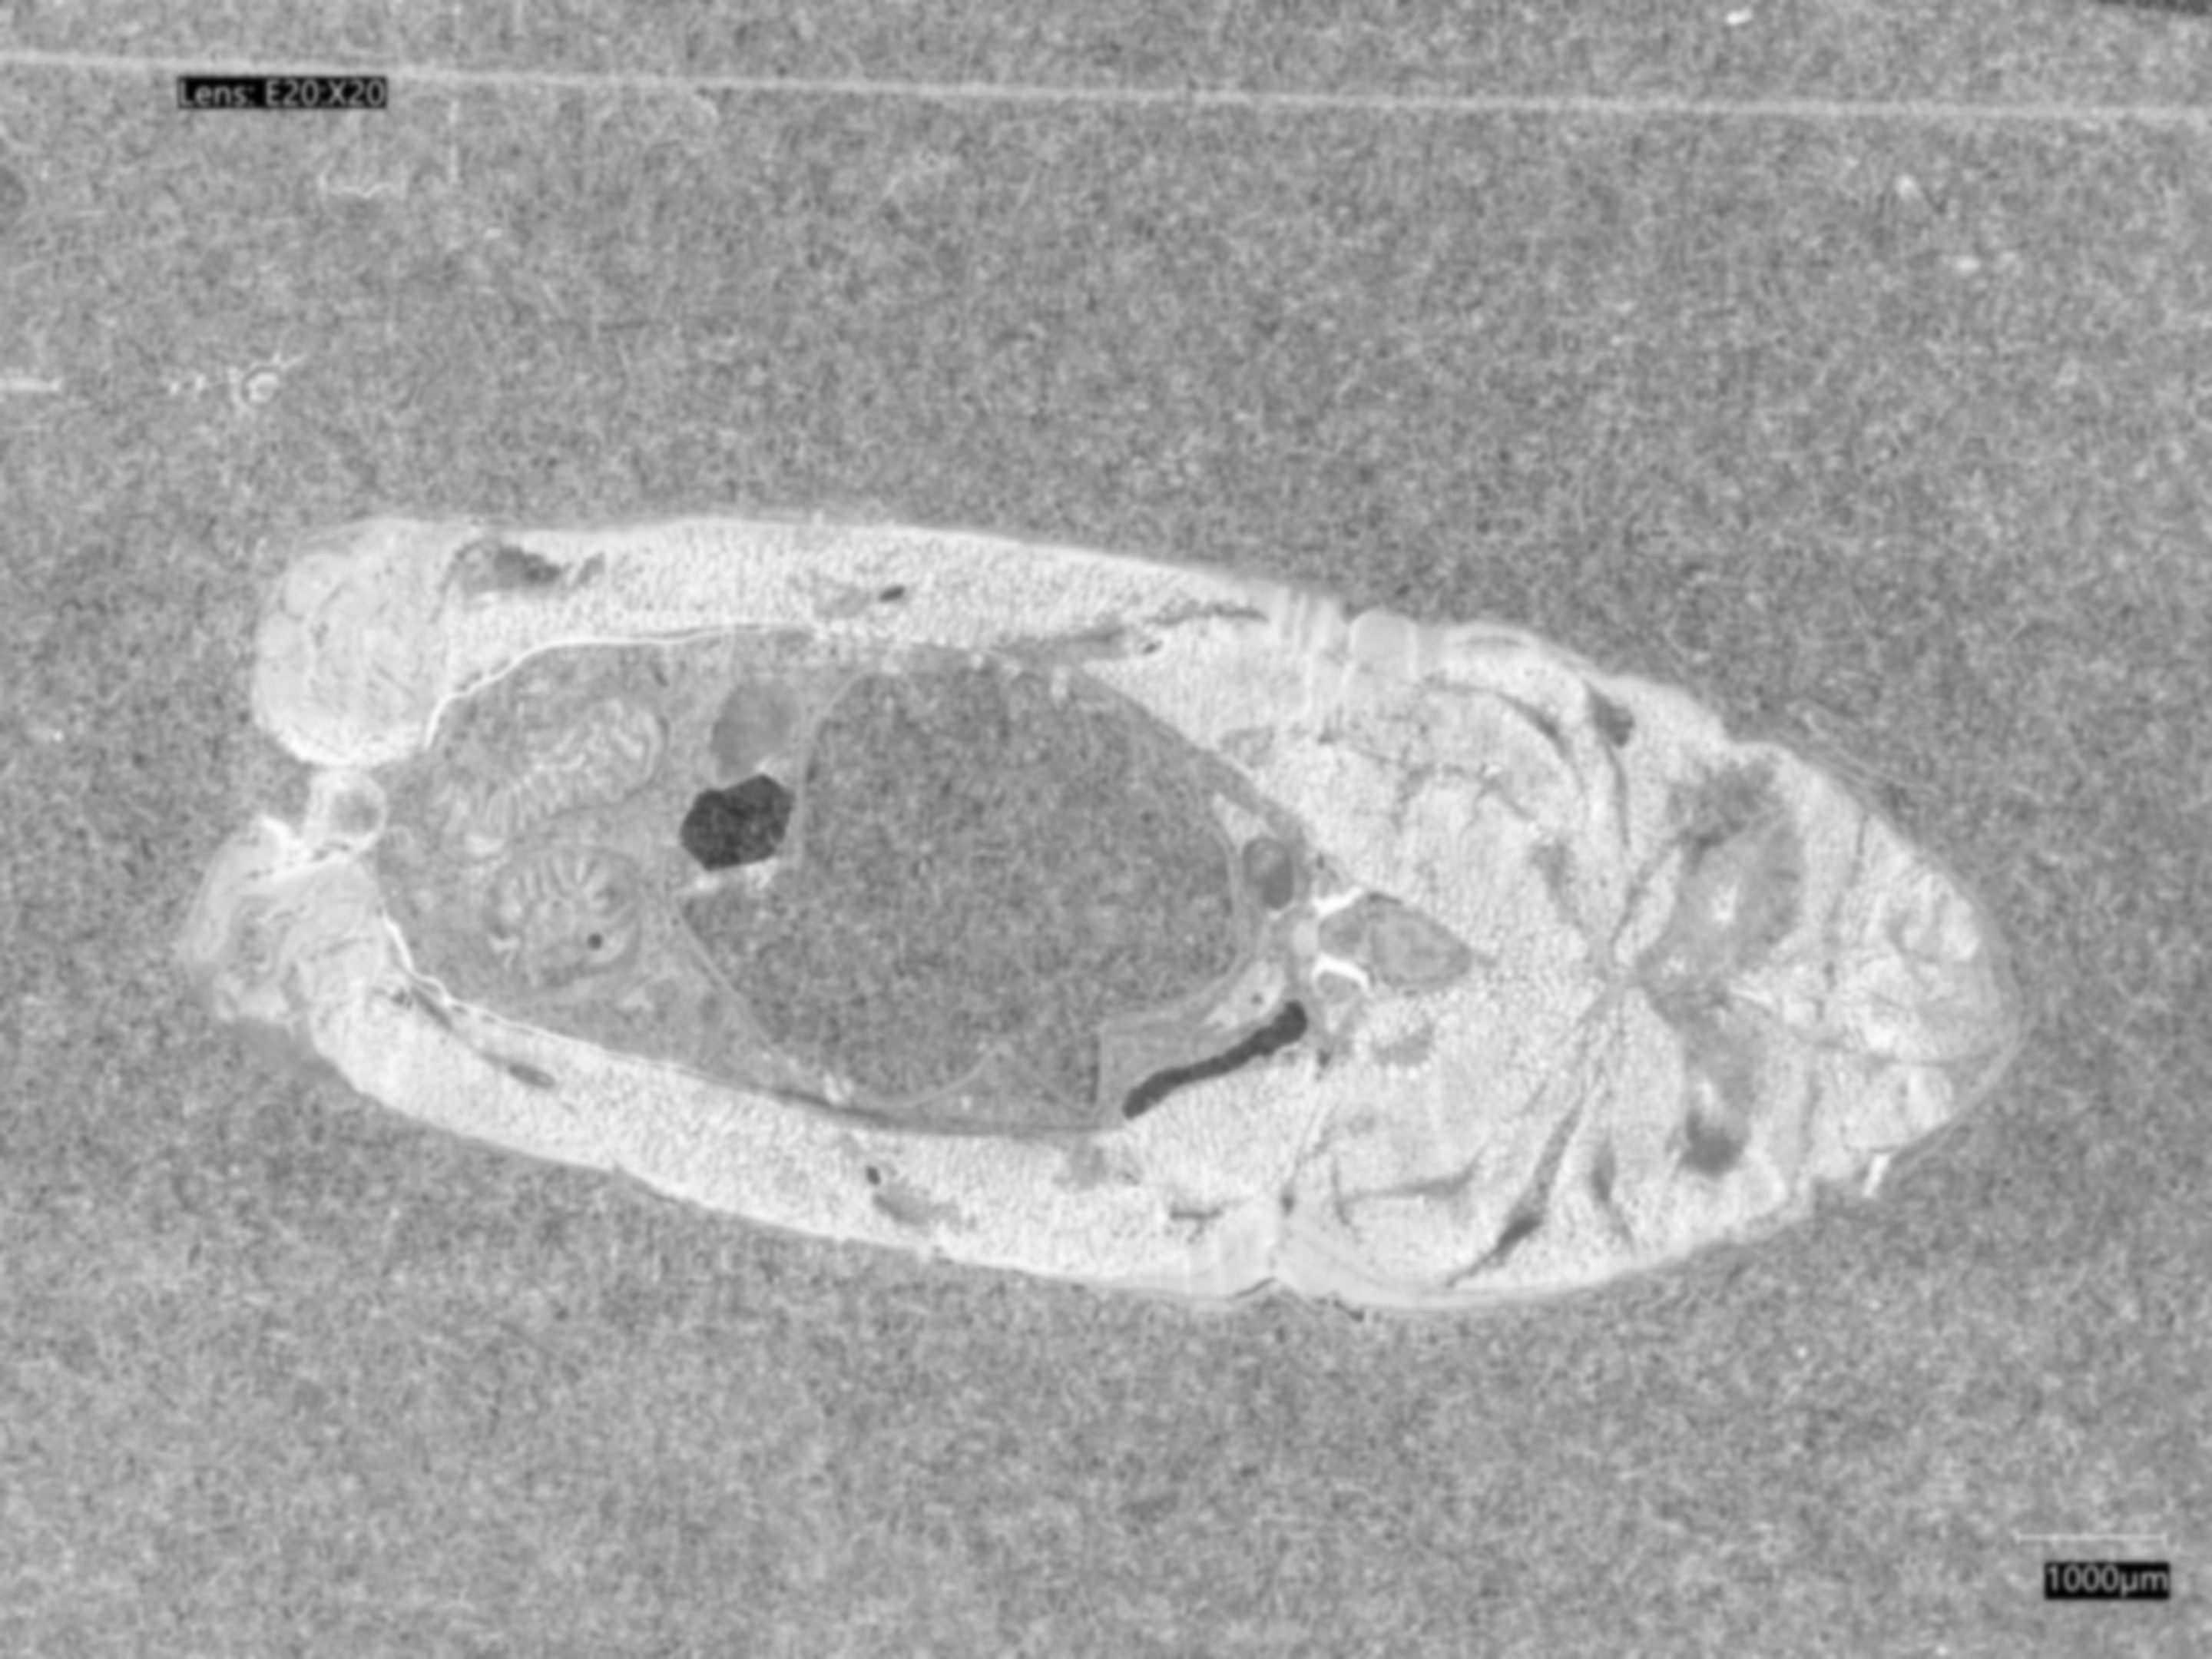
\includegraphics[width=\textwidth]{./fig/gausssian/blurred21.jpg}
        \caption*{k=21}
        % \label{fig:blurred21}
    \end{minipage}
    \begin{minipage}{0.24\textwidth}
        \centering
        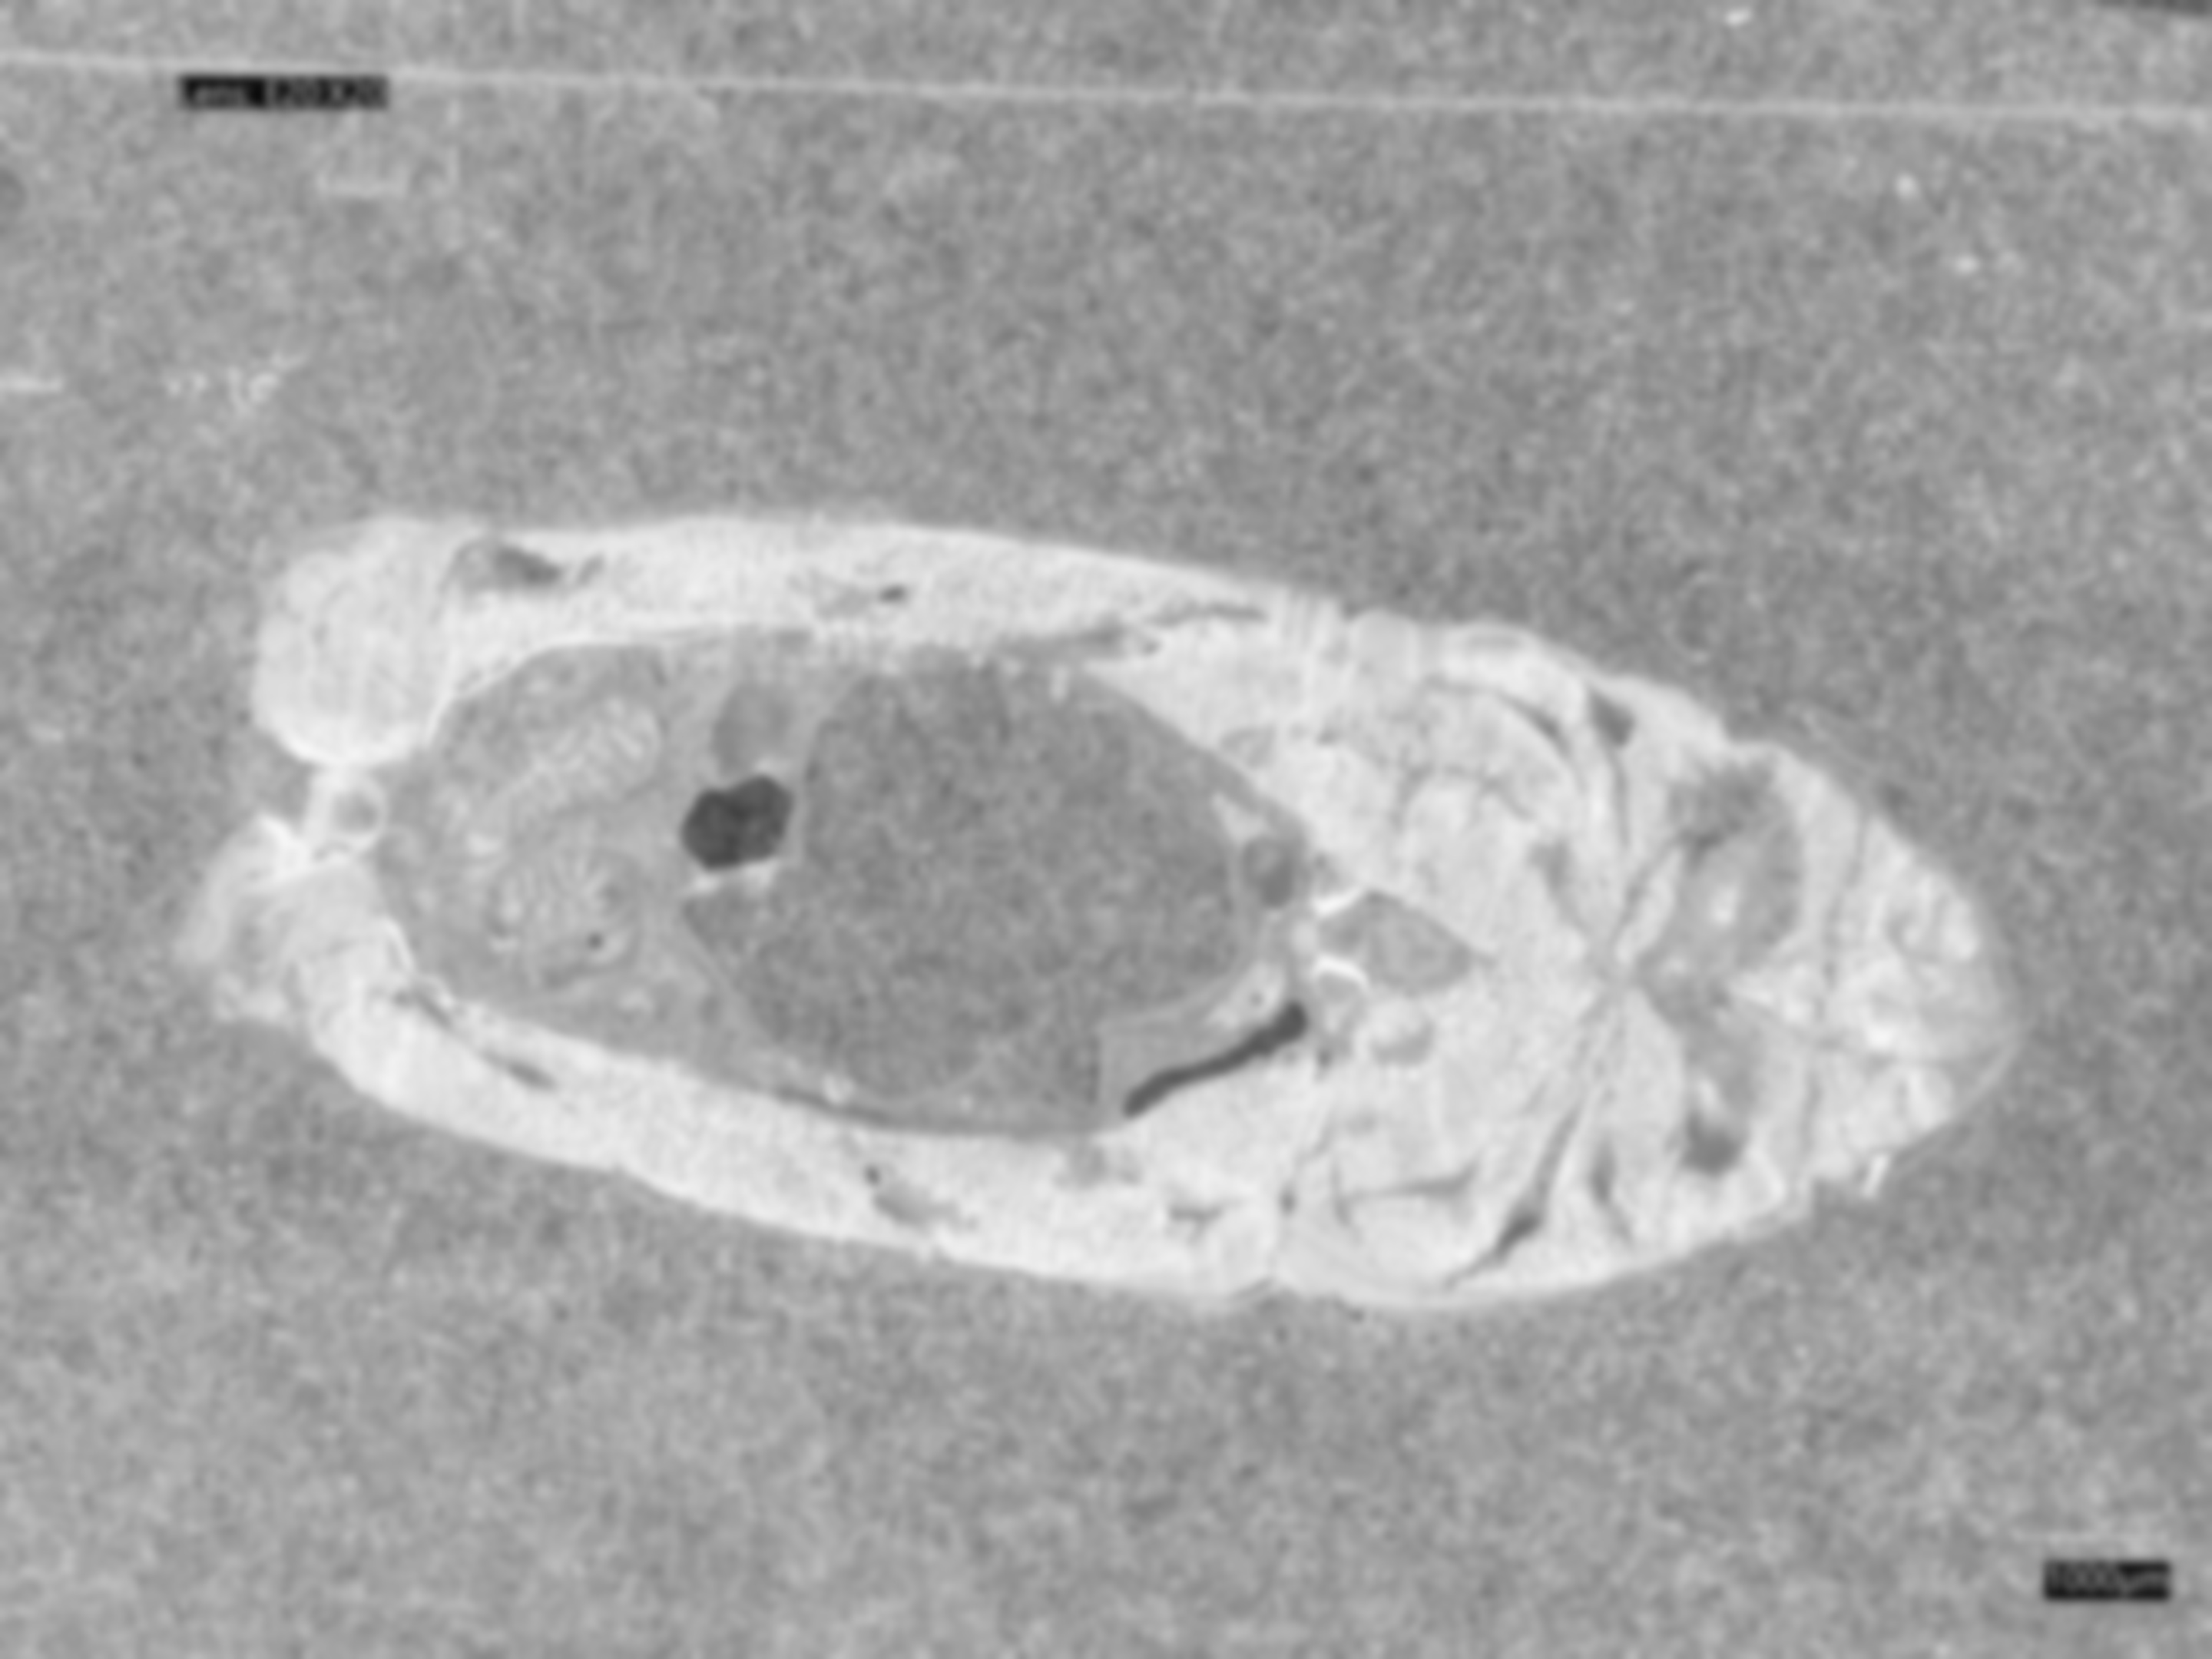
\includegraphics[width=\textwidth]{./fig/gausssian/blurred41.jpg}
        \caption*{k=41}
        % \label{fig:blurred41}
    \end{minipage}
    \begin{minipage}{0.24\textwidth}
        \centering
        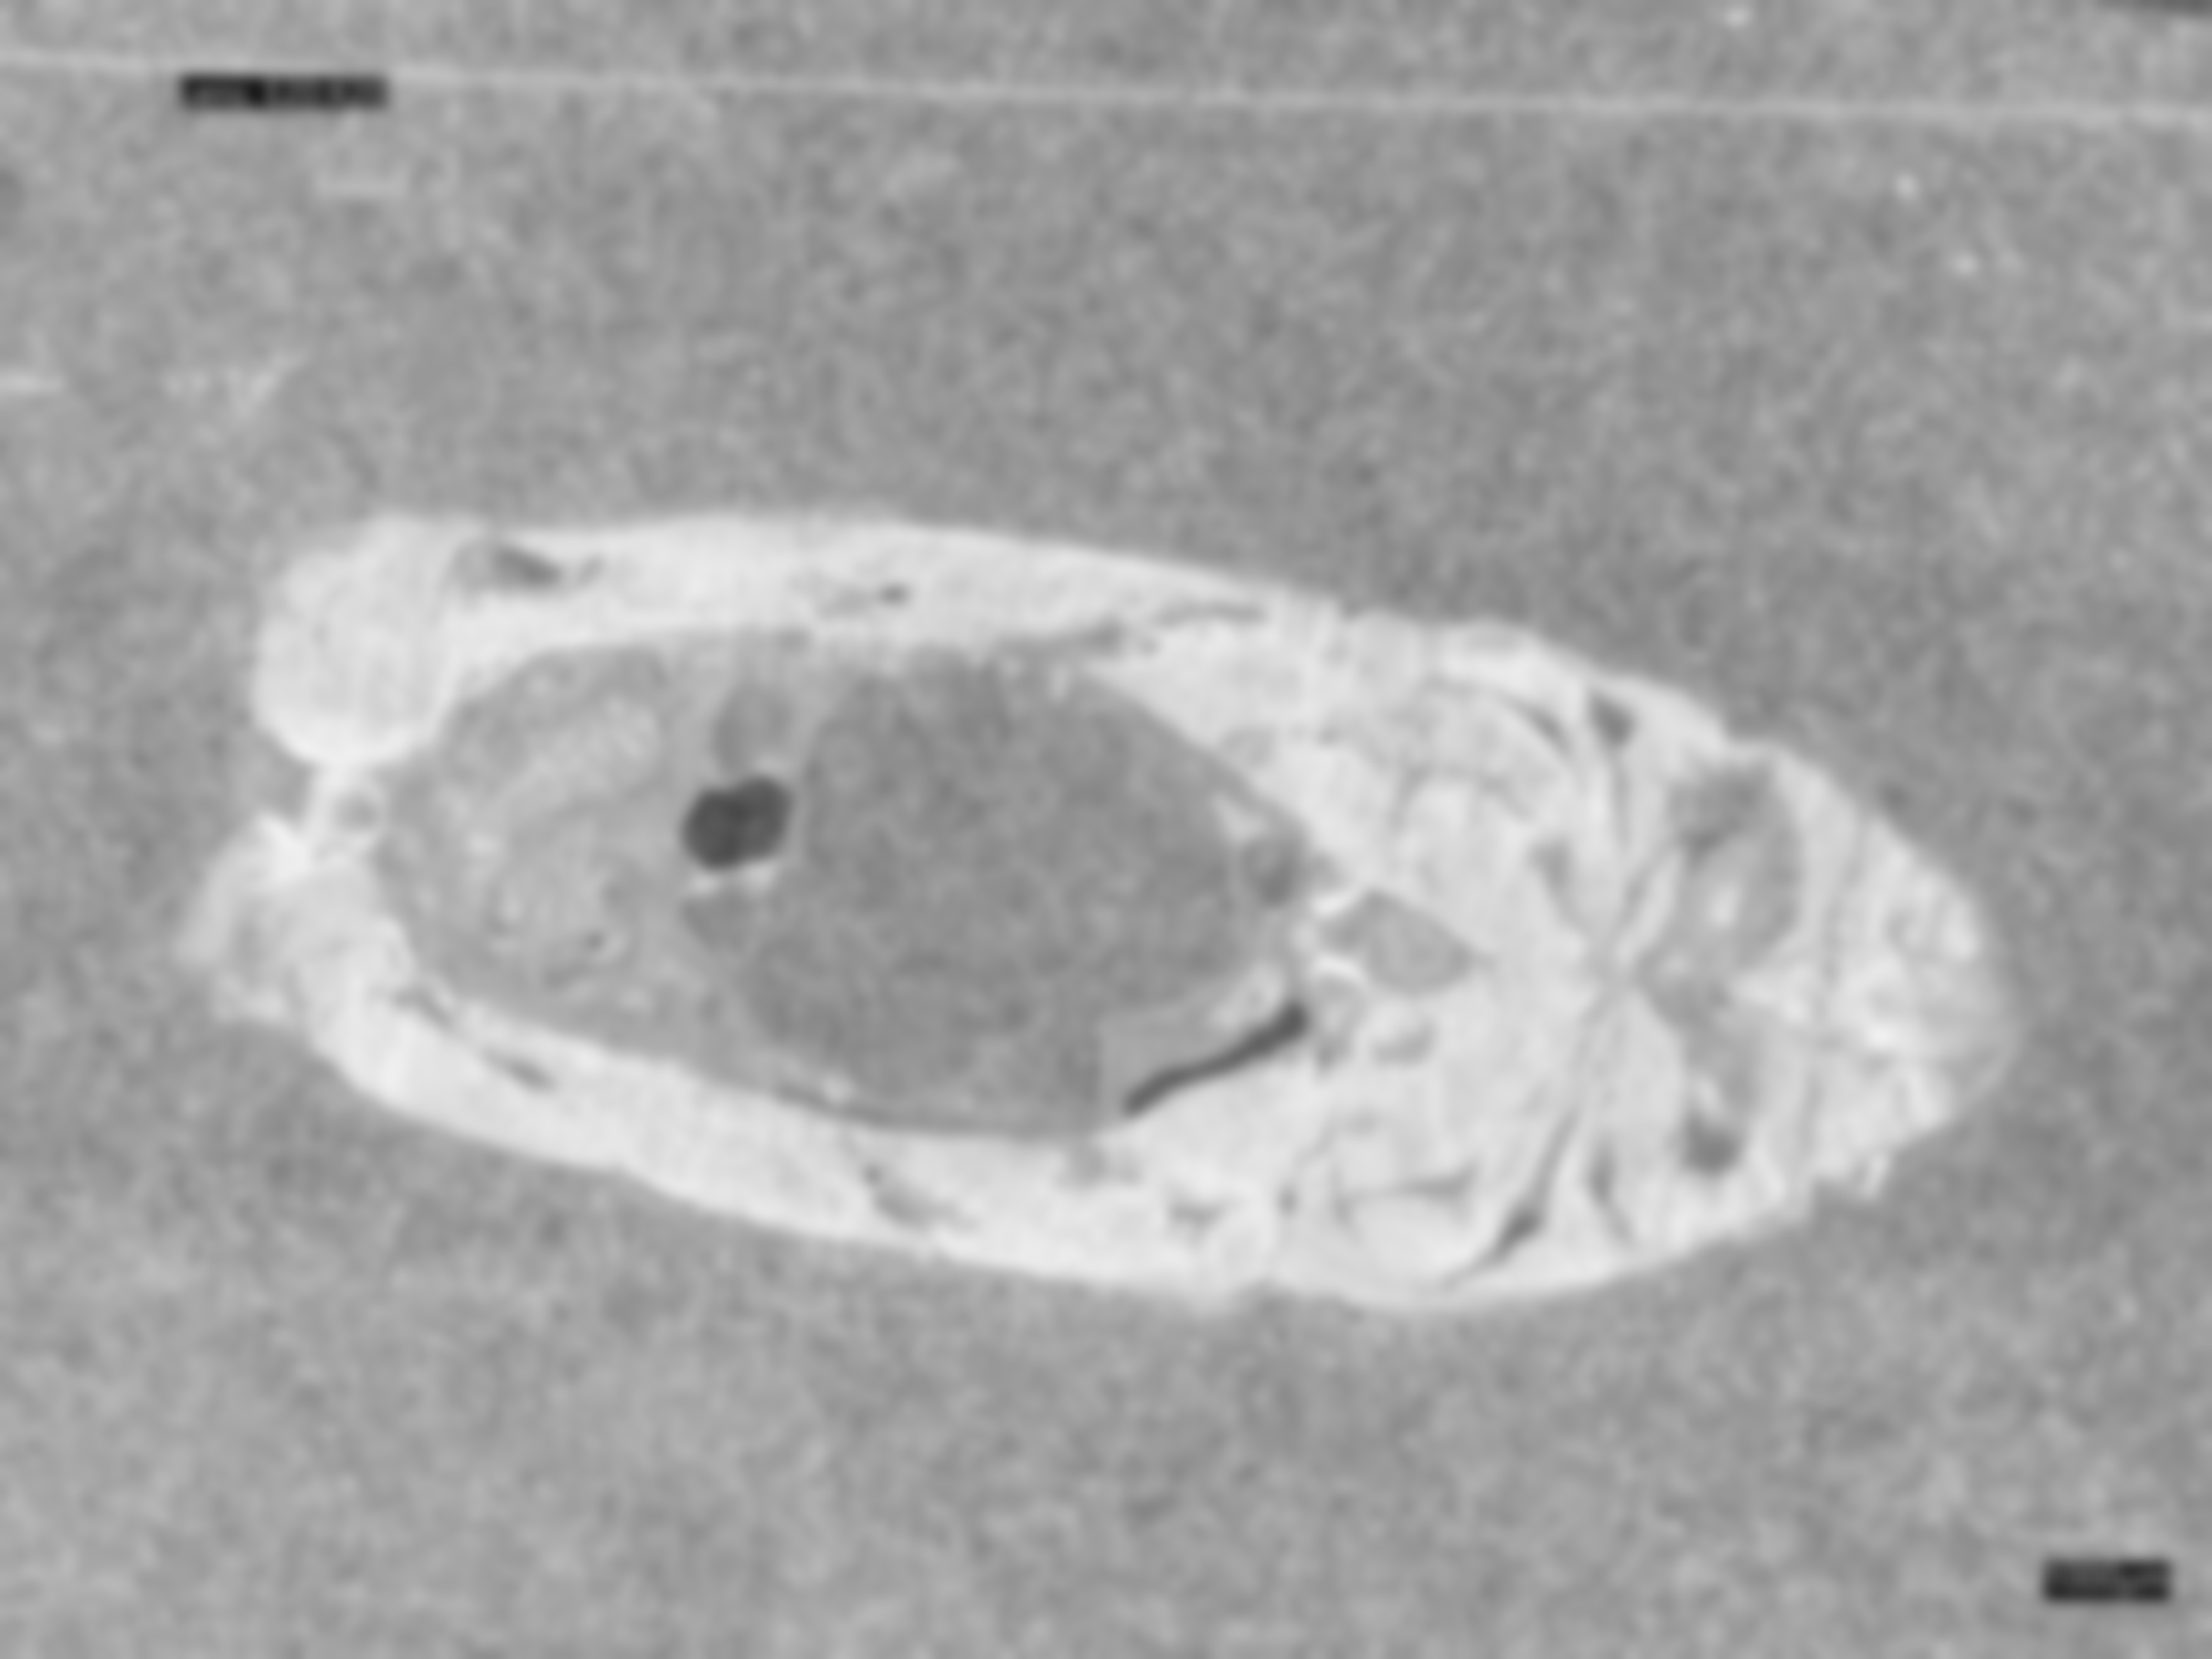
\includegraphics[width=\textwidth]{./fig/gausssian/blurred61.jpg}
        \caption*{k=61}
        % \label{fig:blurred61}
    \end{minipage}
    \begin{minipage}{0.24\textwidth}
        \centering
        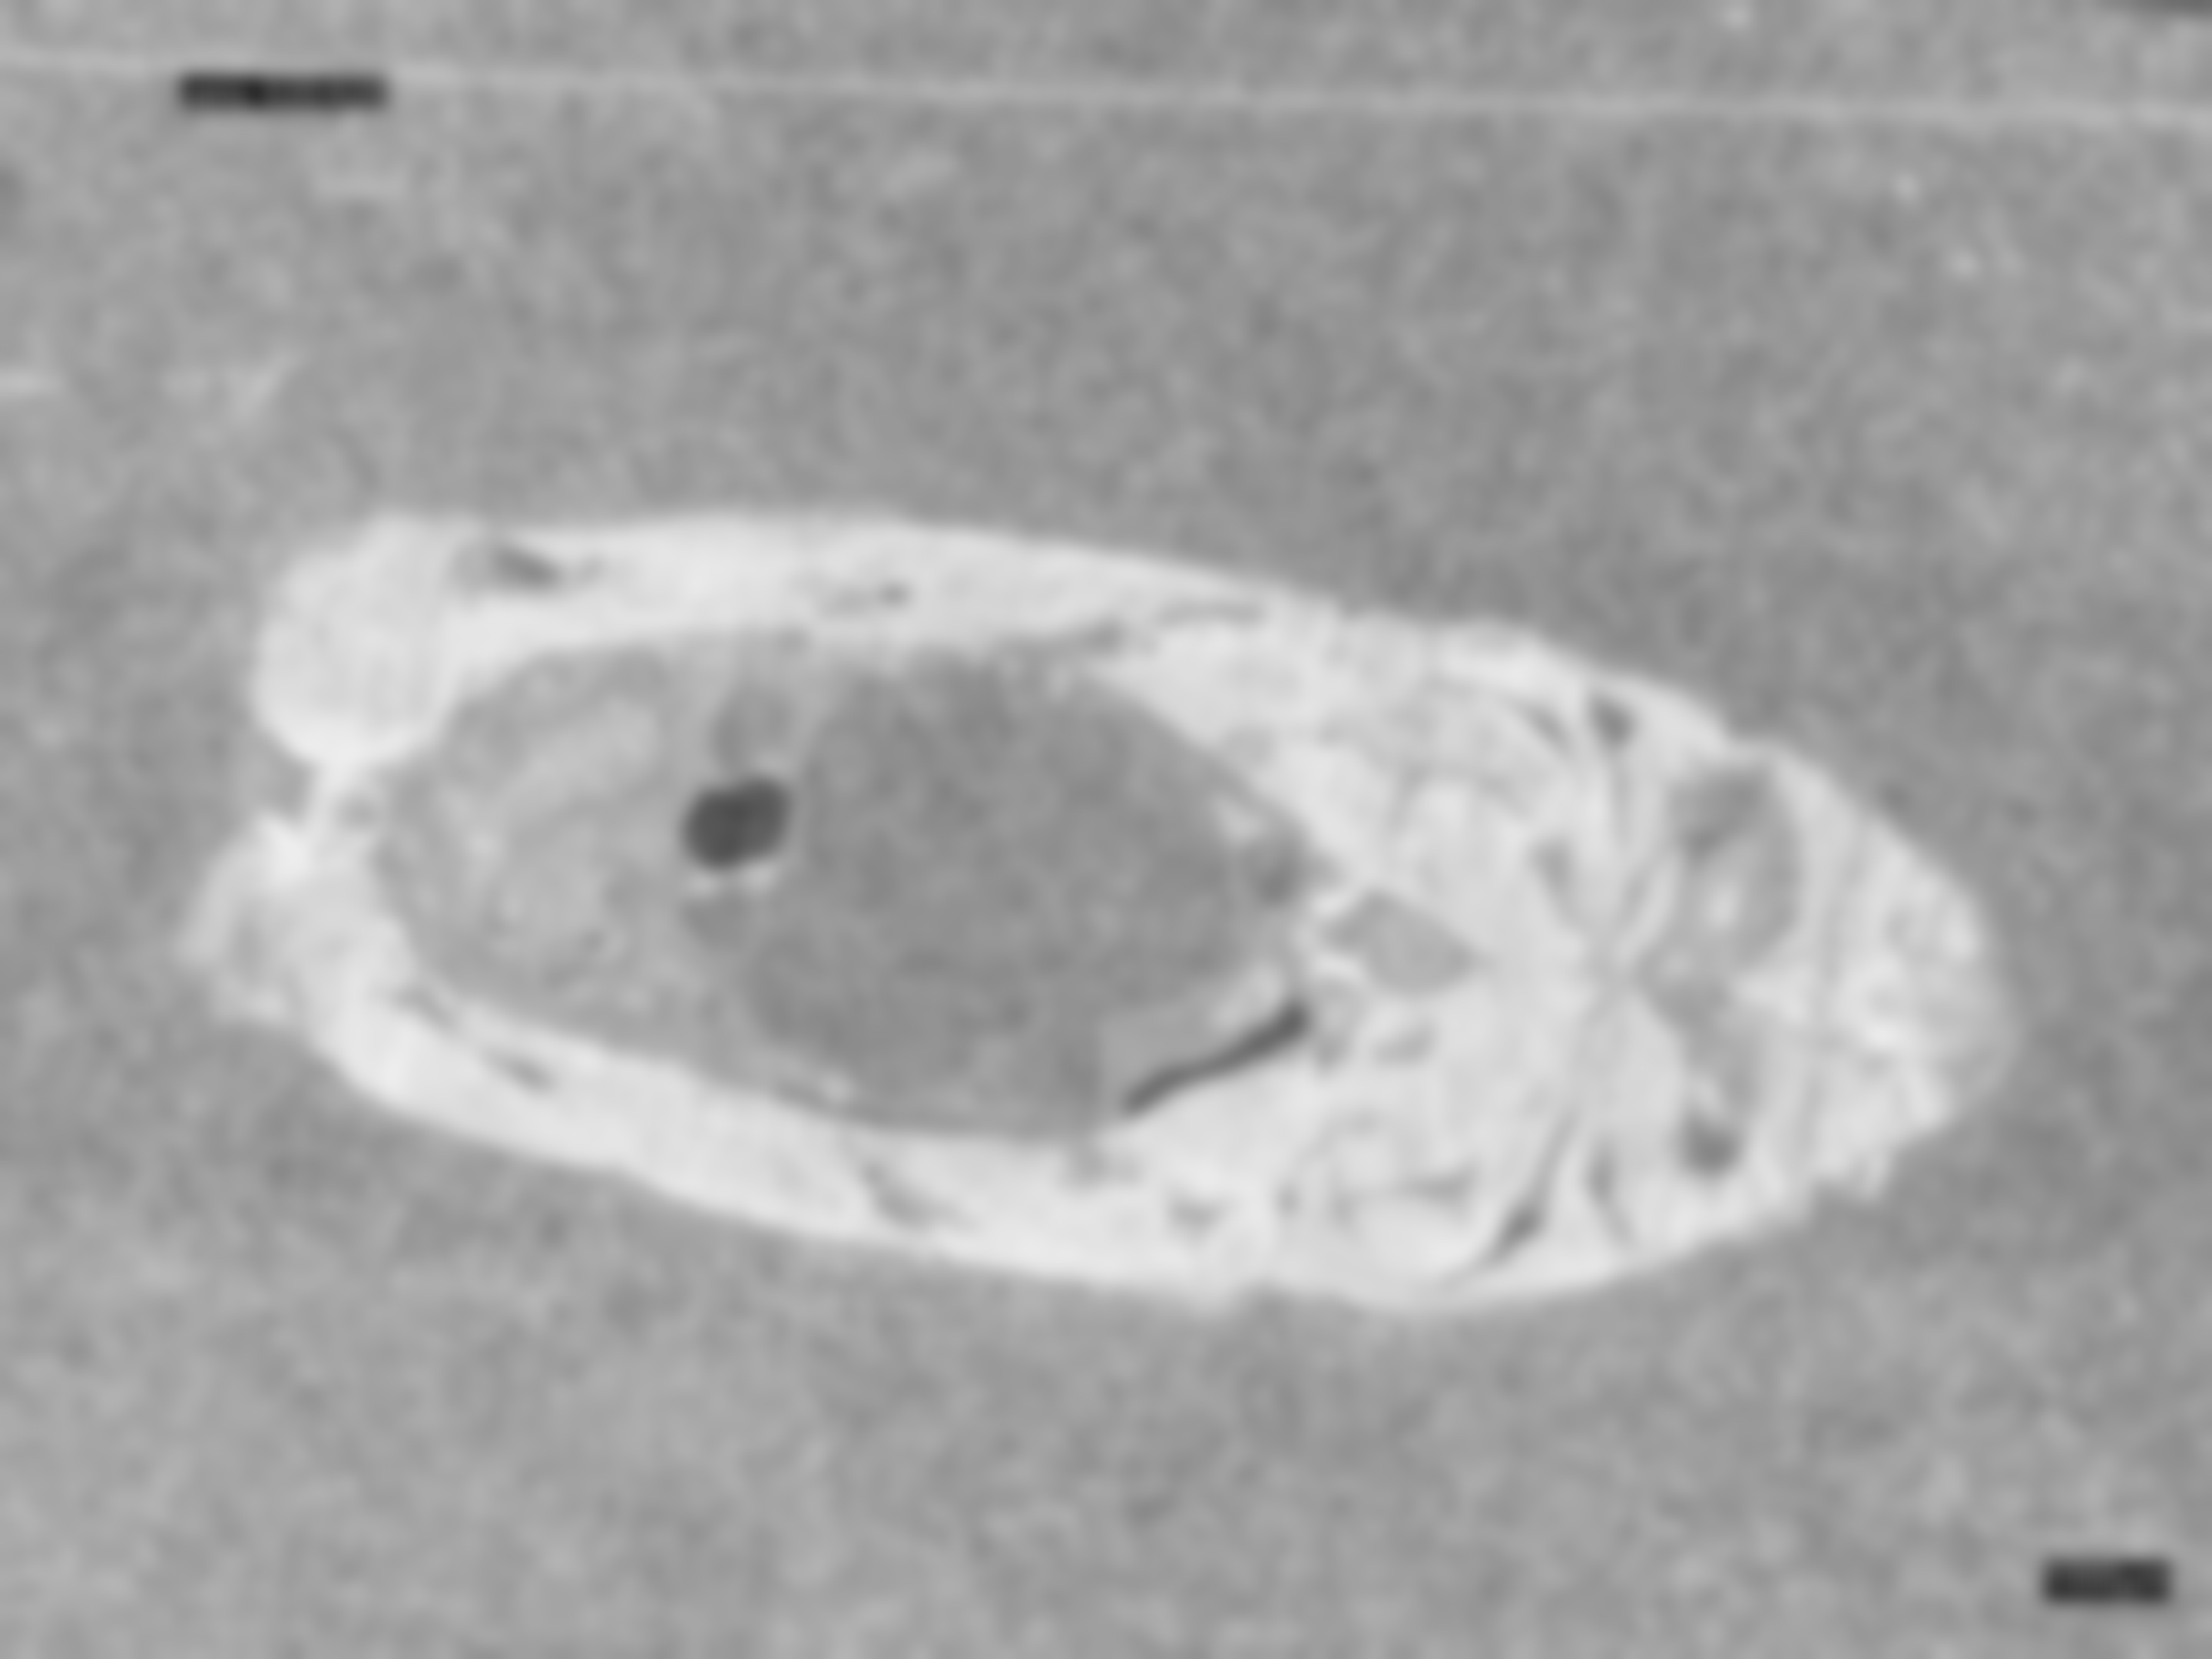
\includegraphics[width=\textwidth]{./fig/gausssian/blurred81.jpg}
        \caption*{k=81}
        % \label{fig:blurred81}
    \end{minipage}
    \caption{Images post-Gaussian blur}
    \label{fig:blurred}
\end{figure}

\begin{figure}
    \centering
    \begin{minipage}{0.24\textwidth}
        \centering
        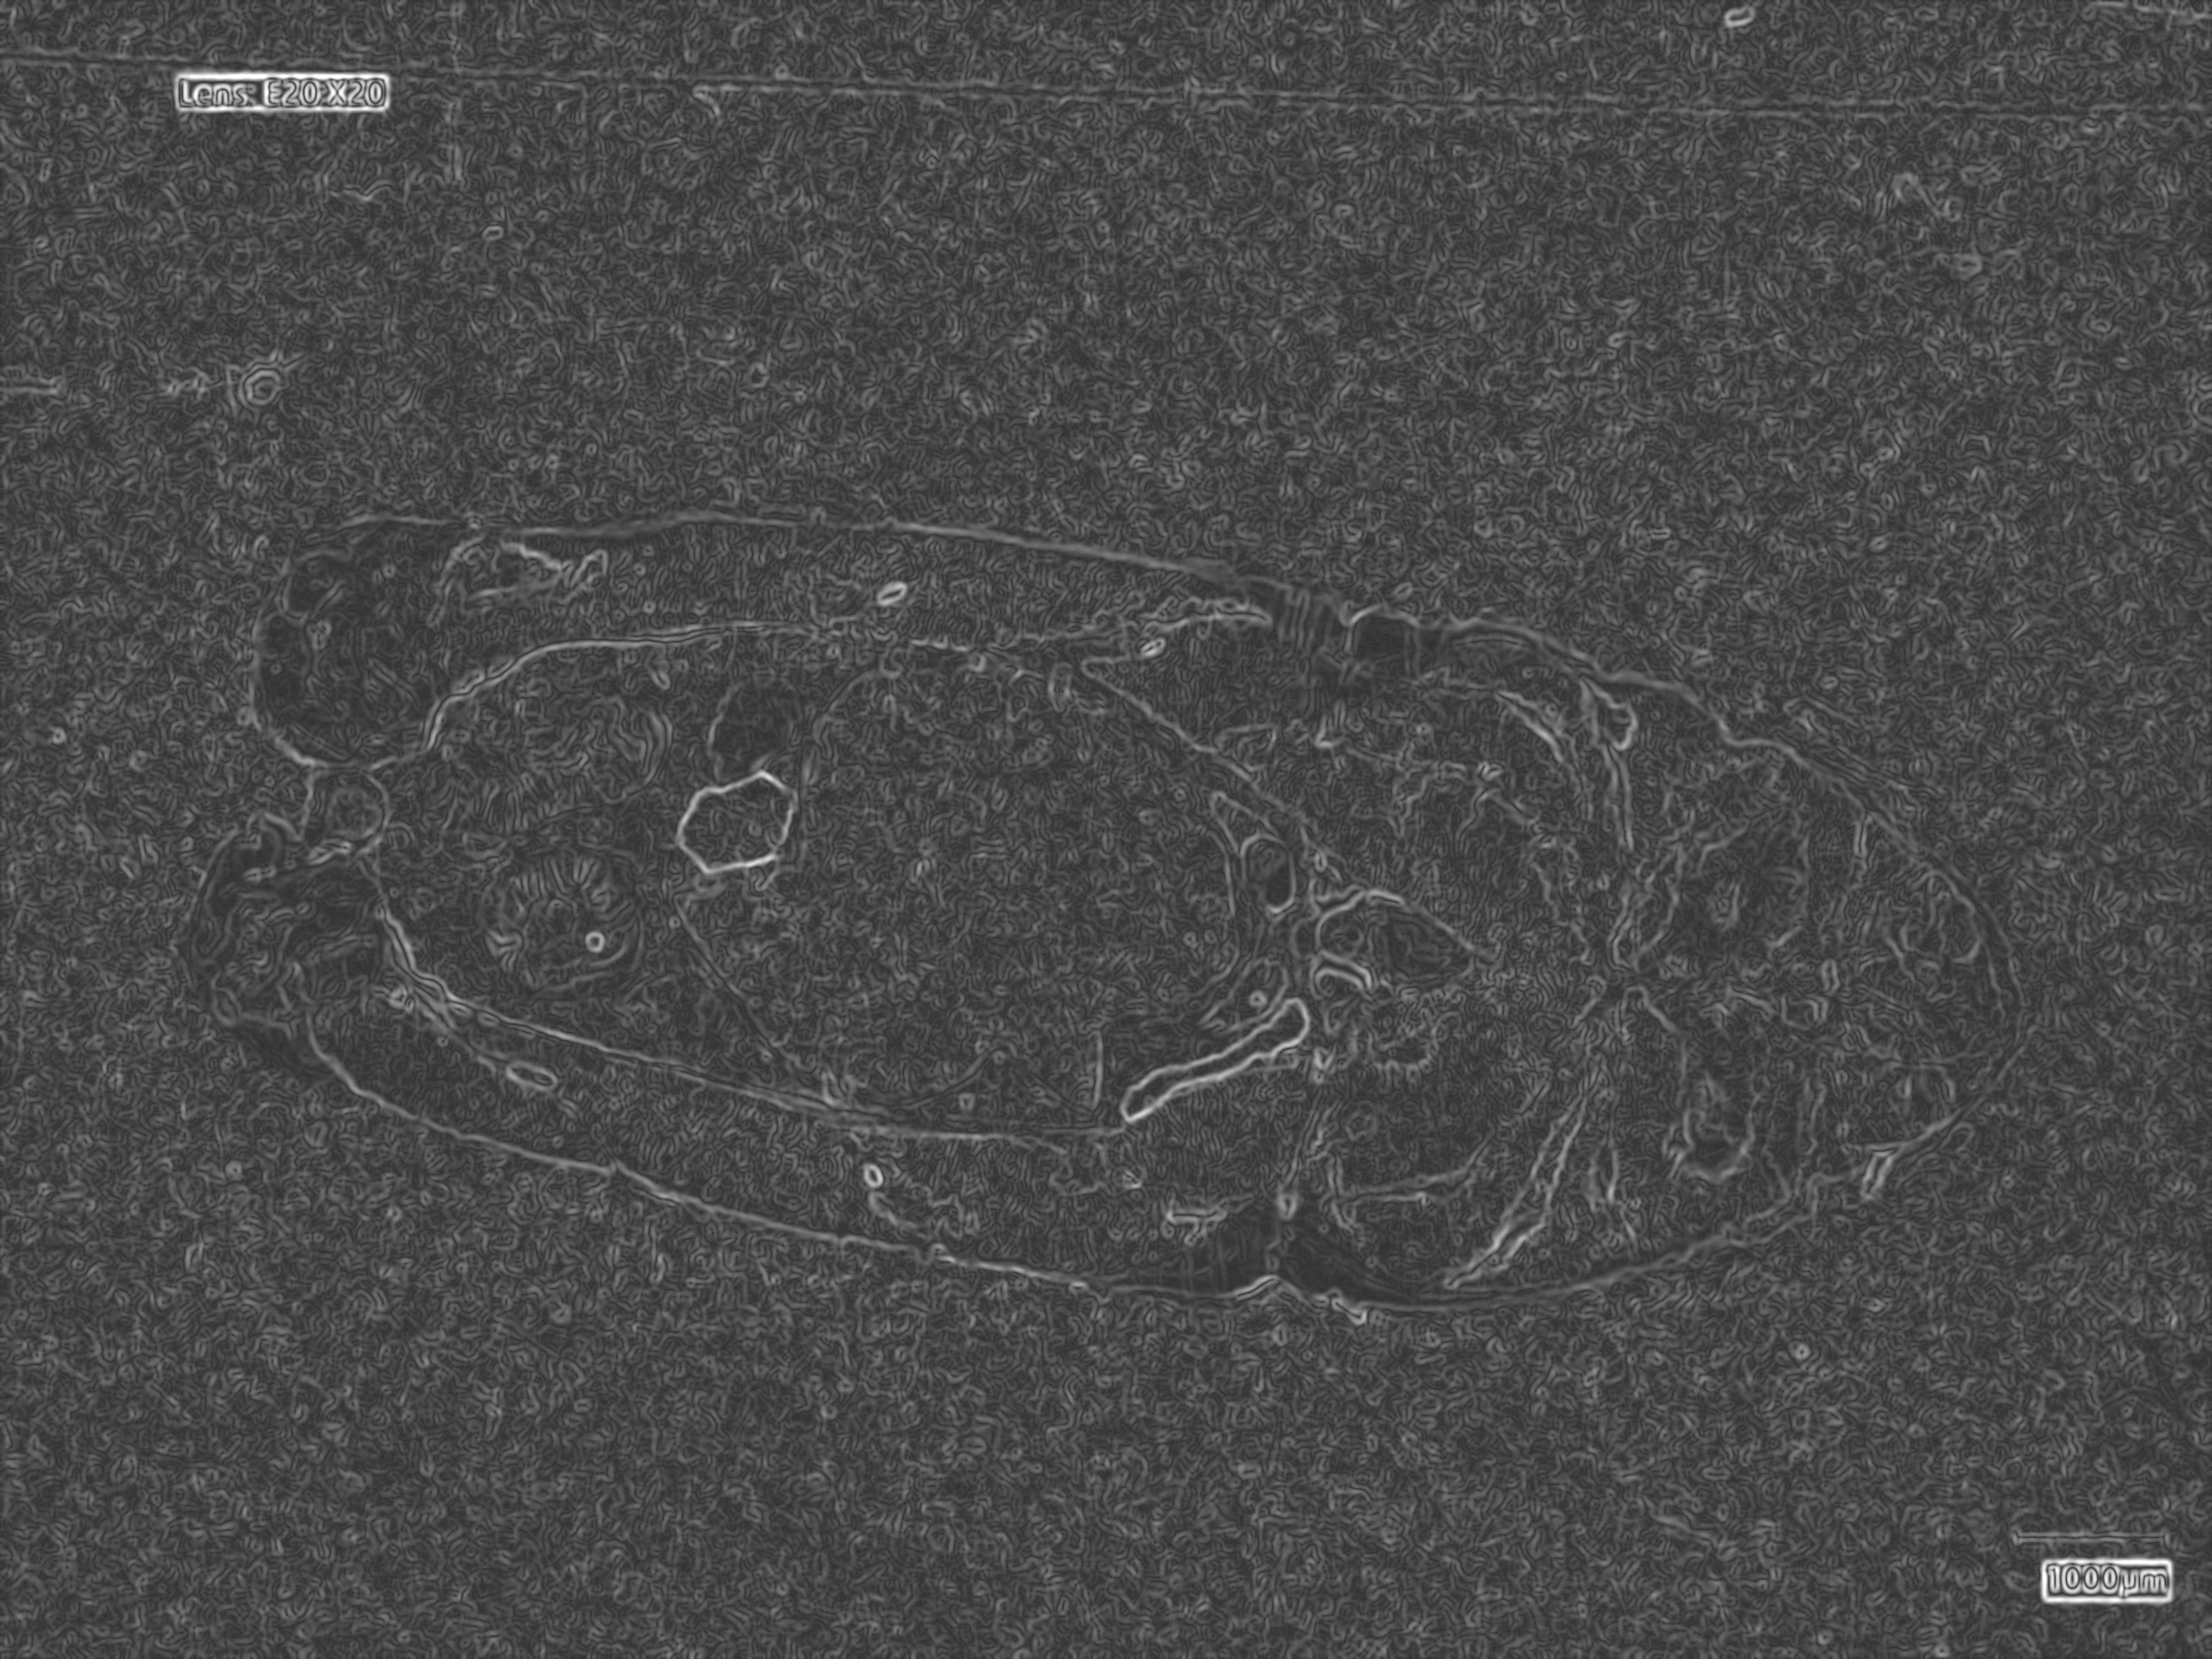
\includegraphics[width=\textwidth]{./fig/gausssian/sobel21.jpg}
        \caption*{k=21}
        % \label{fig:sobel21}
    \end{minipage}
    \begin{minipage}{0.24\textwidth}
        \centering
        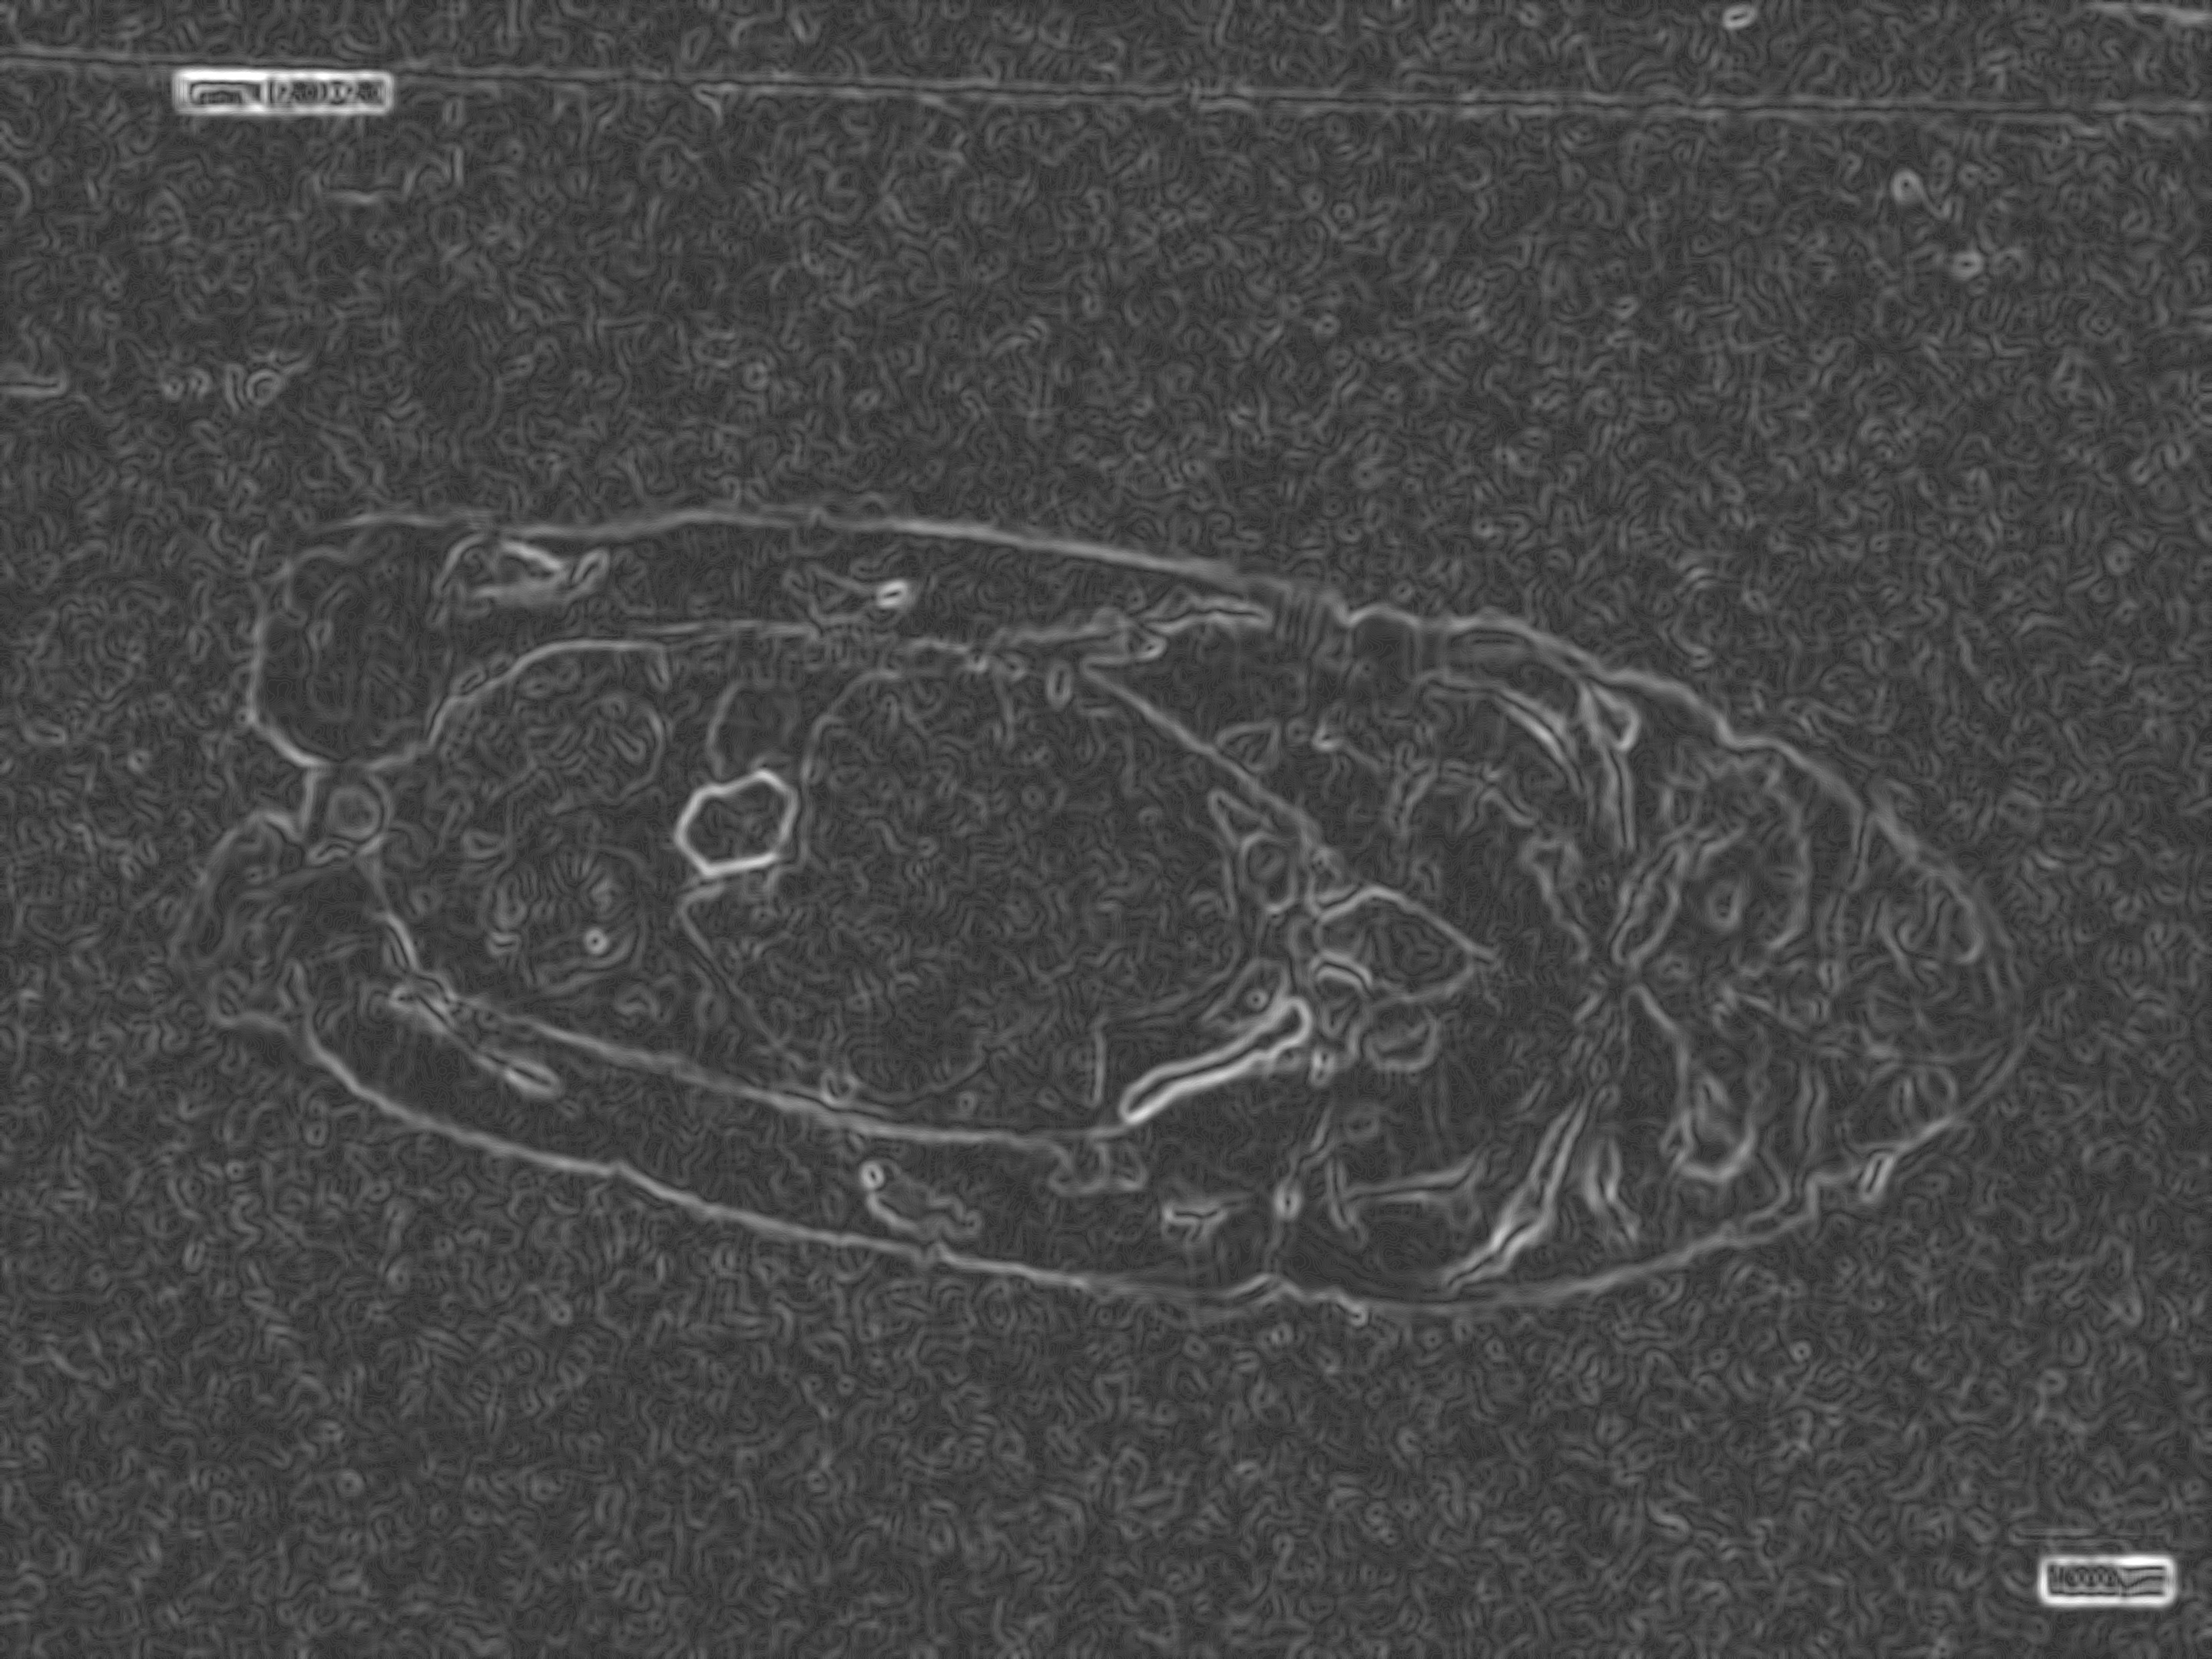
\includegraphics[width=\textwidth]{./fig/gausssian/sobel41.jpg}
        \caption*{k=41}
        % \label{fig:sobel41}
    \end{minipage}
    \begin{minipage}{0.24\textwidth}
        \centering
        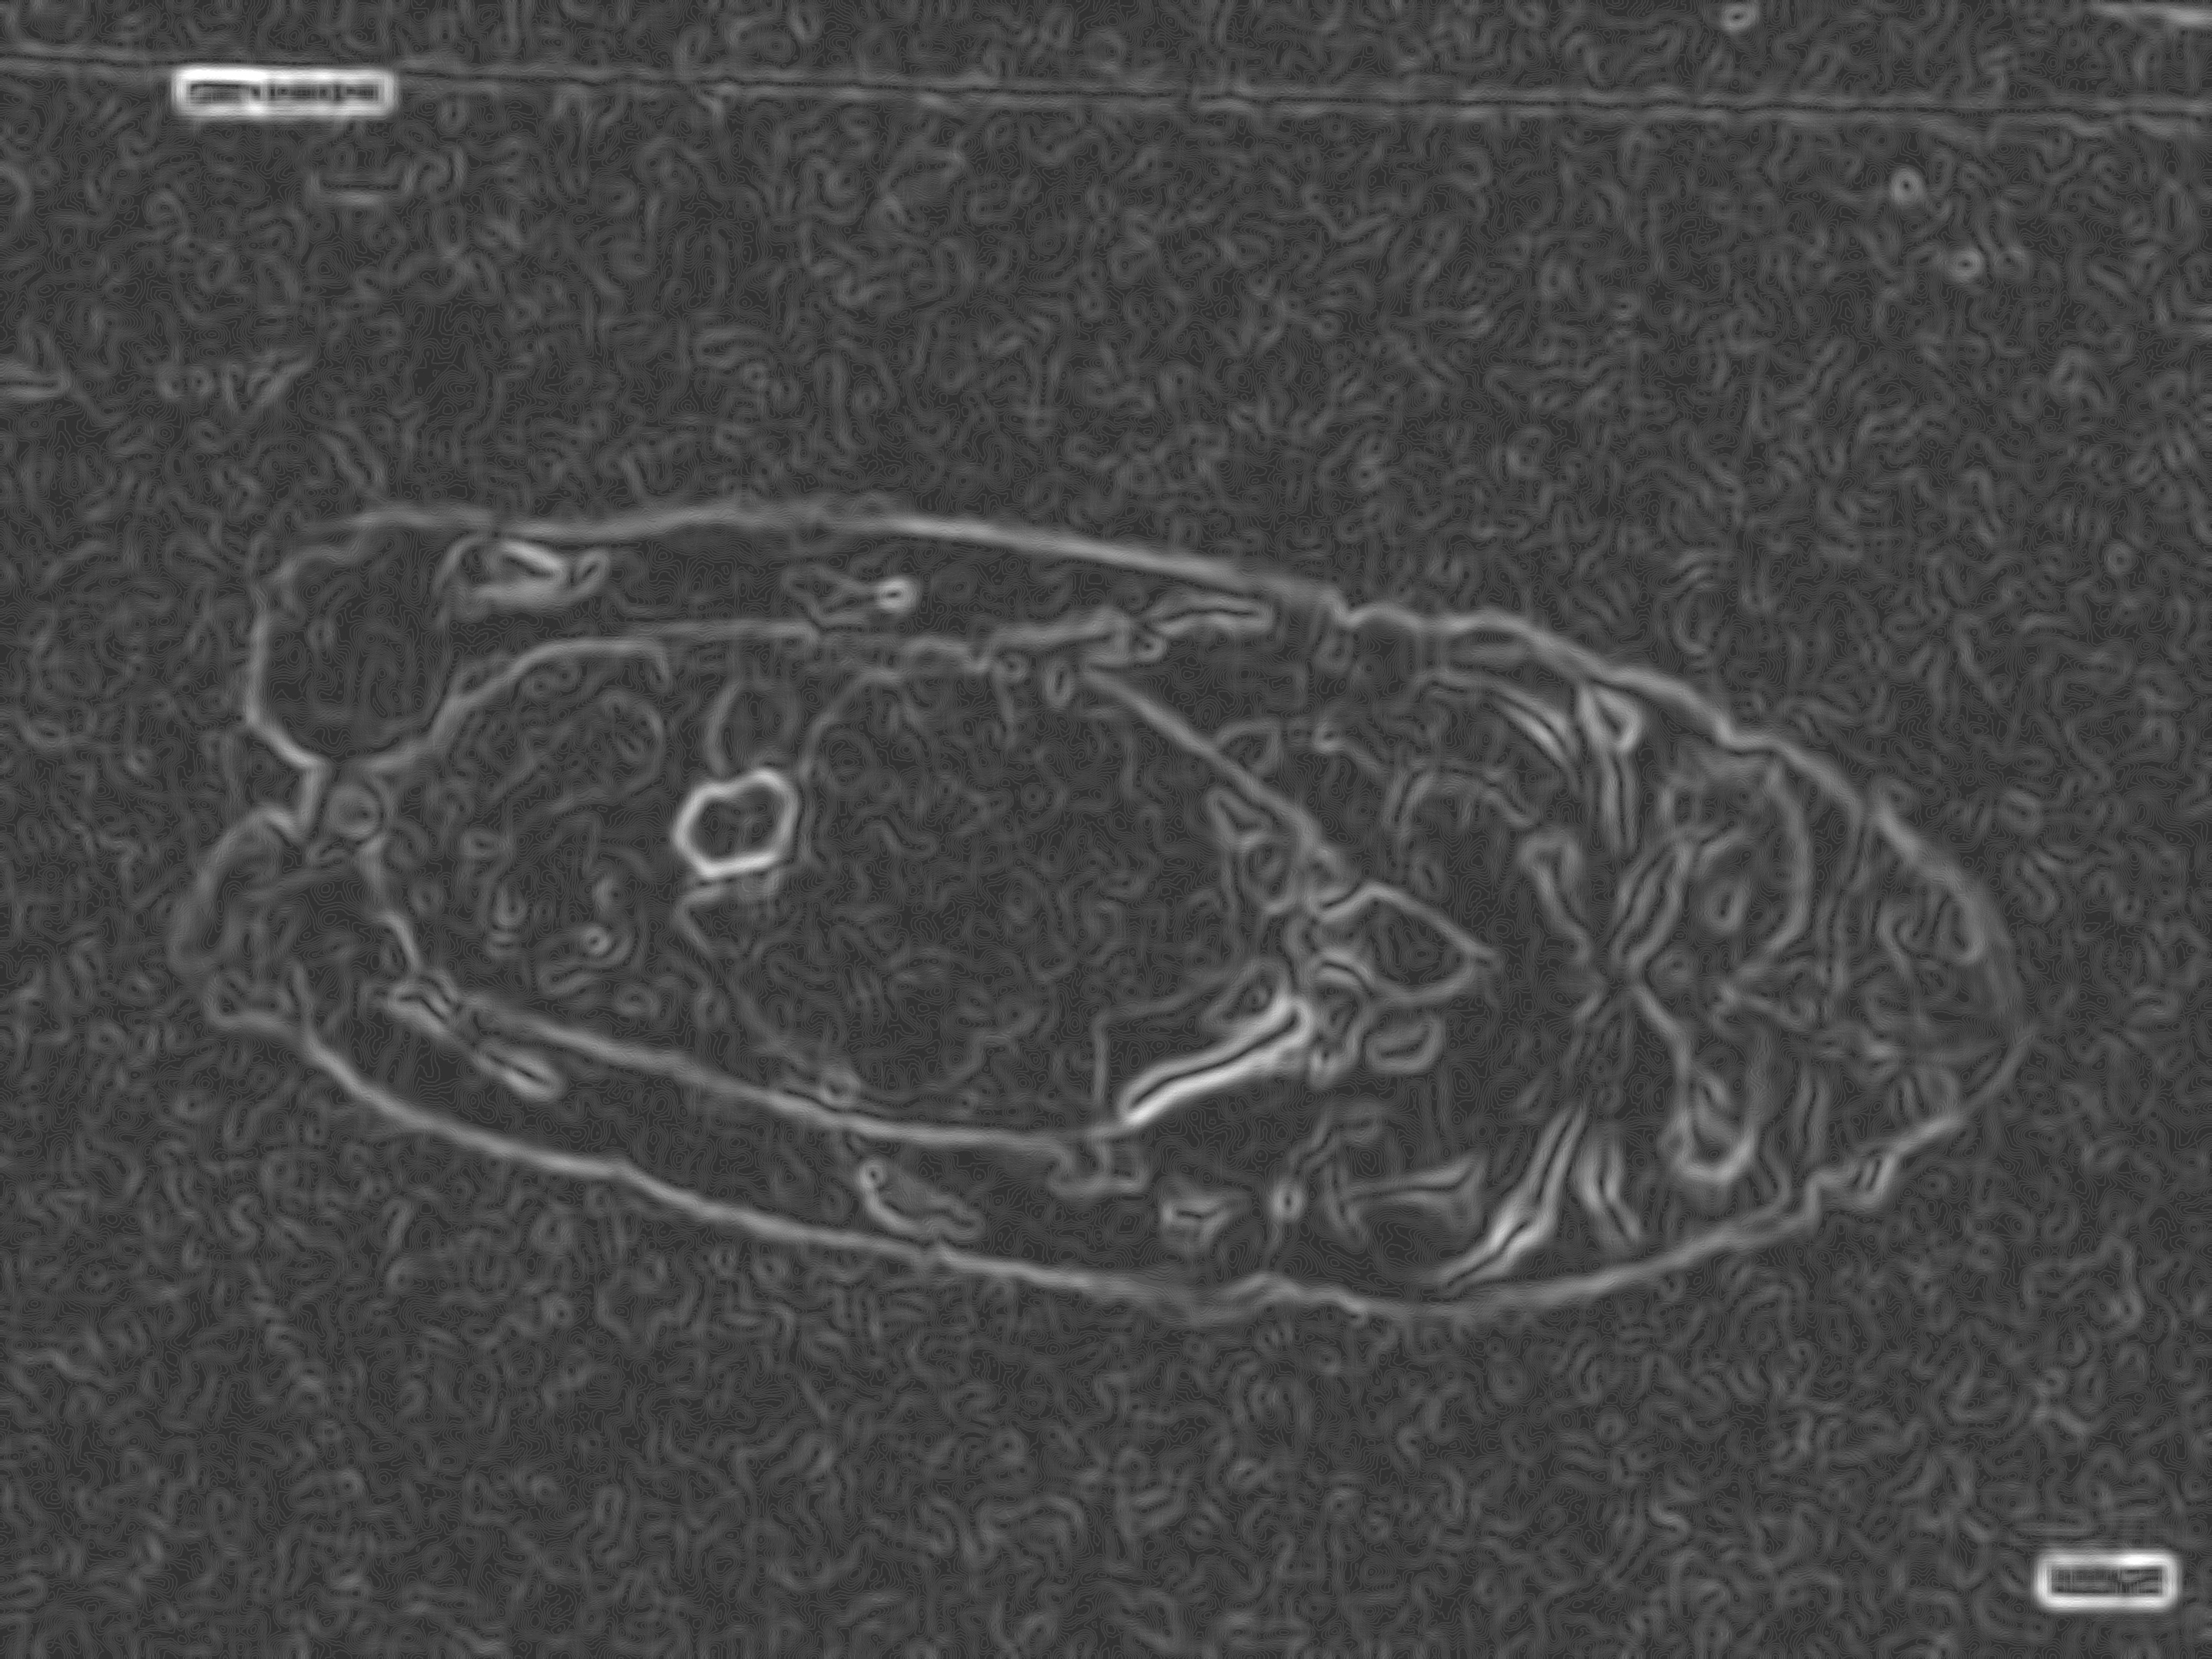
\includegraphics[width=\textwidth]{./fig/gausssian/sobel61.jpg}
        \caption*{k=61}
        % \label{fig:sobel61}
    \end{minipage}
    \begin{minipage}{0.24\textwidth}
        \centering
        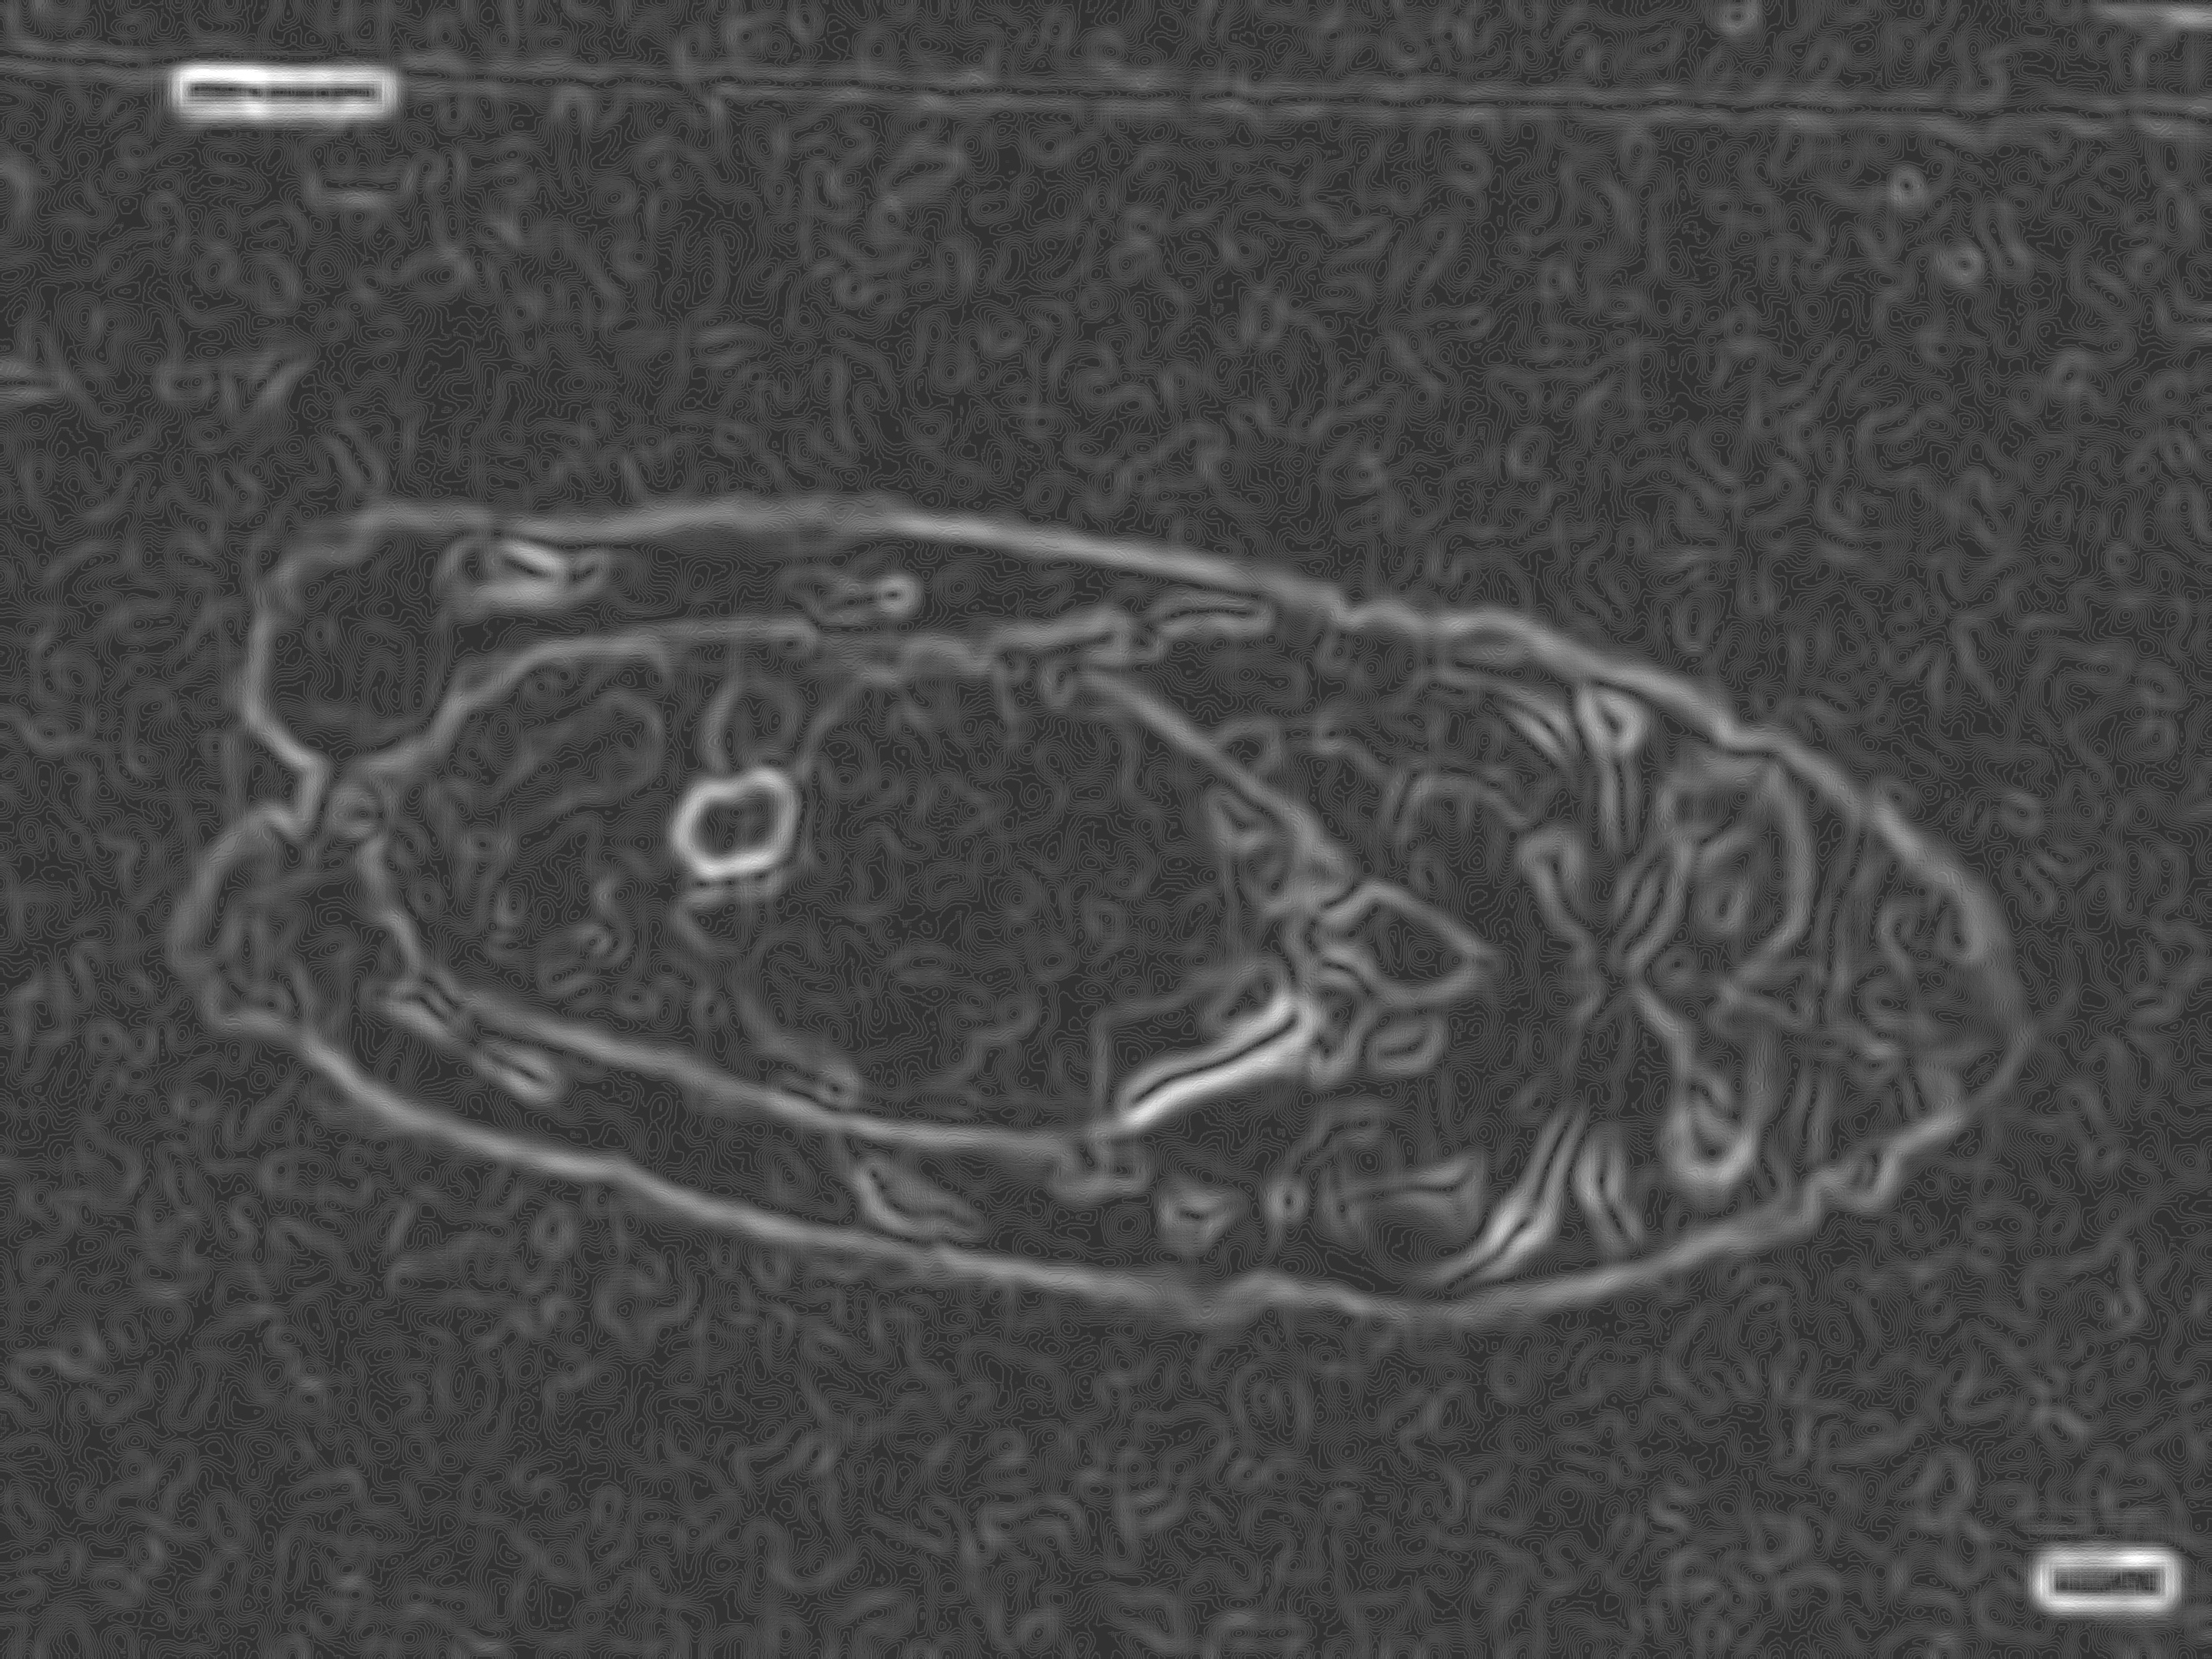
\includegraphics[width=\textwidth]{./fig/gausssian/sobel81.jpg}
        \caption*{k=81}
        % \label{fig:sobel81}
    \end{minipage}
    \caption{Images post-Sobel operator}
    \label{fig:sobel}
\end{figure}

In \autoref{fig:blurred}, it can be observed that as the Gaussian blur kernel size increases, the image details become progressively more blurred, and the edges also become more indistinct. In \autoref{fig:sobel} the effectiveness of edge detection diminishes as the kernel size increases, with the edges becoming less prominent. Considering the clarity of image edges against background noise, a Gaussian kernel size of 61 is selected.


Following the application of Gaussian blur (k=61), the results using the Laplacian operator via Python's OpenCV library are depicted below:

\begin{figure}[H]
\centering
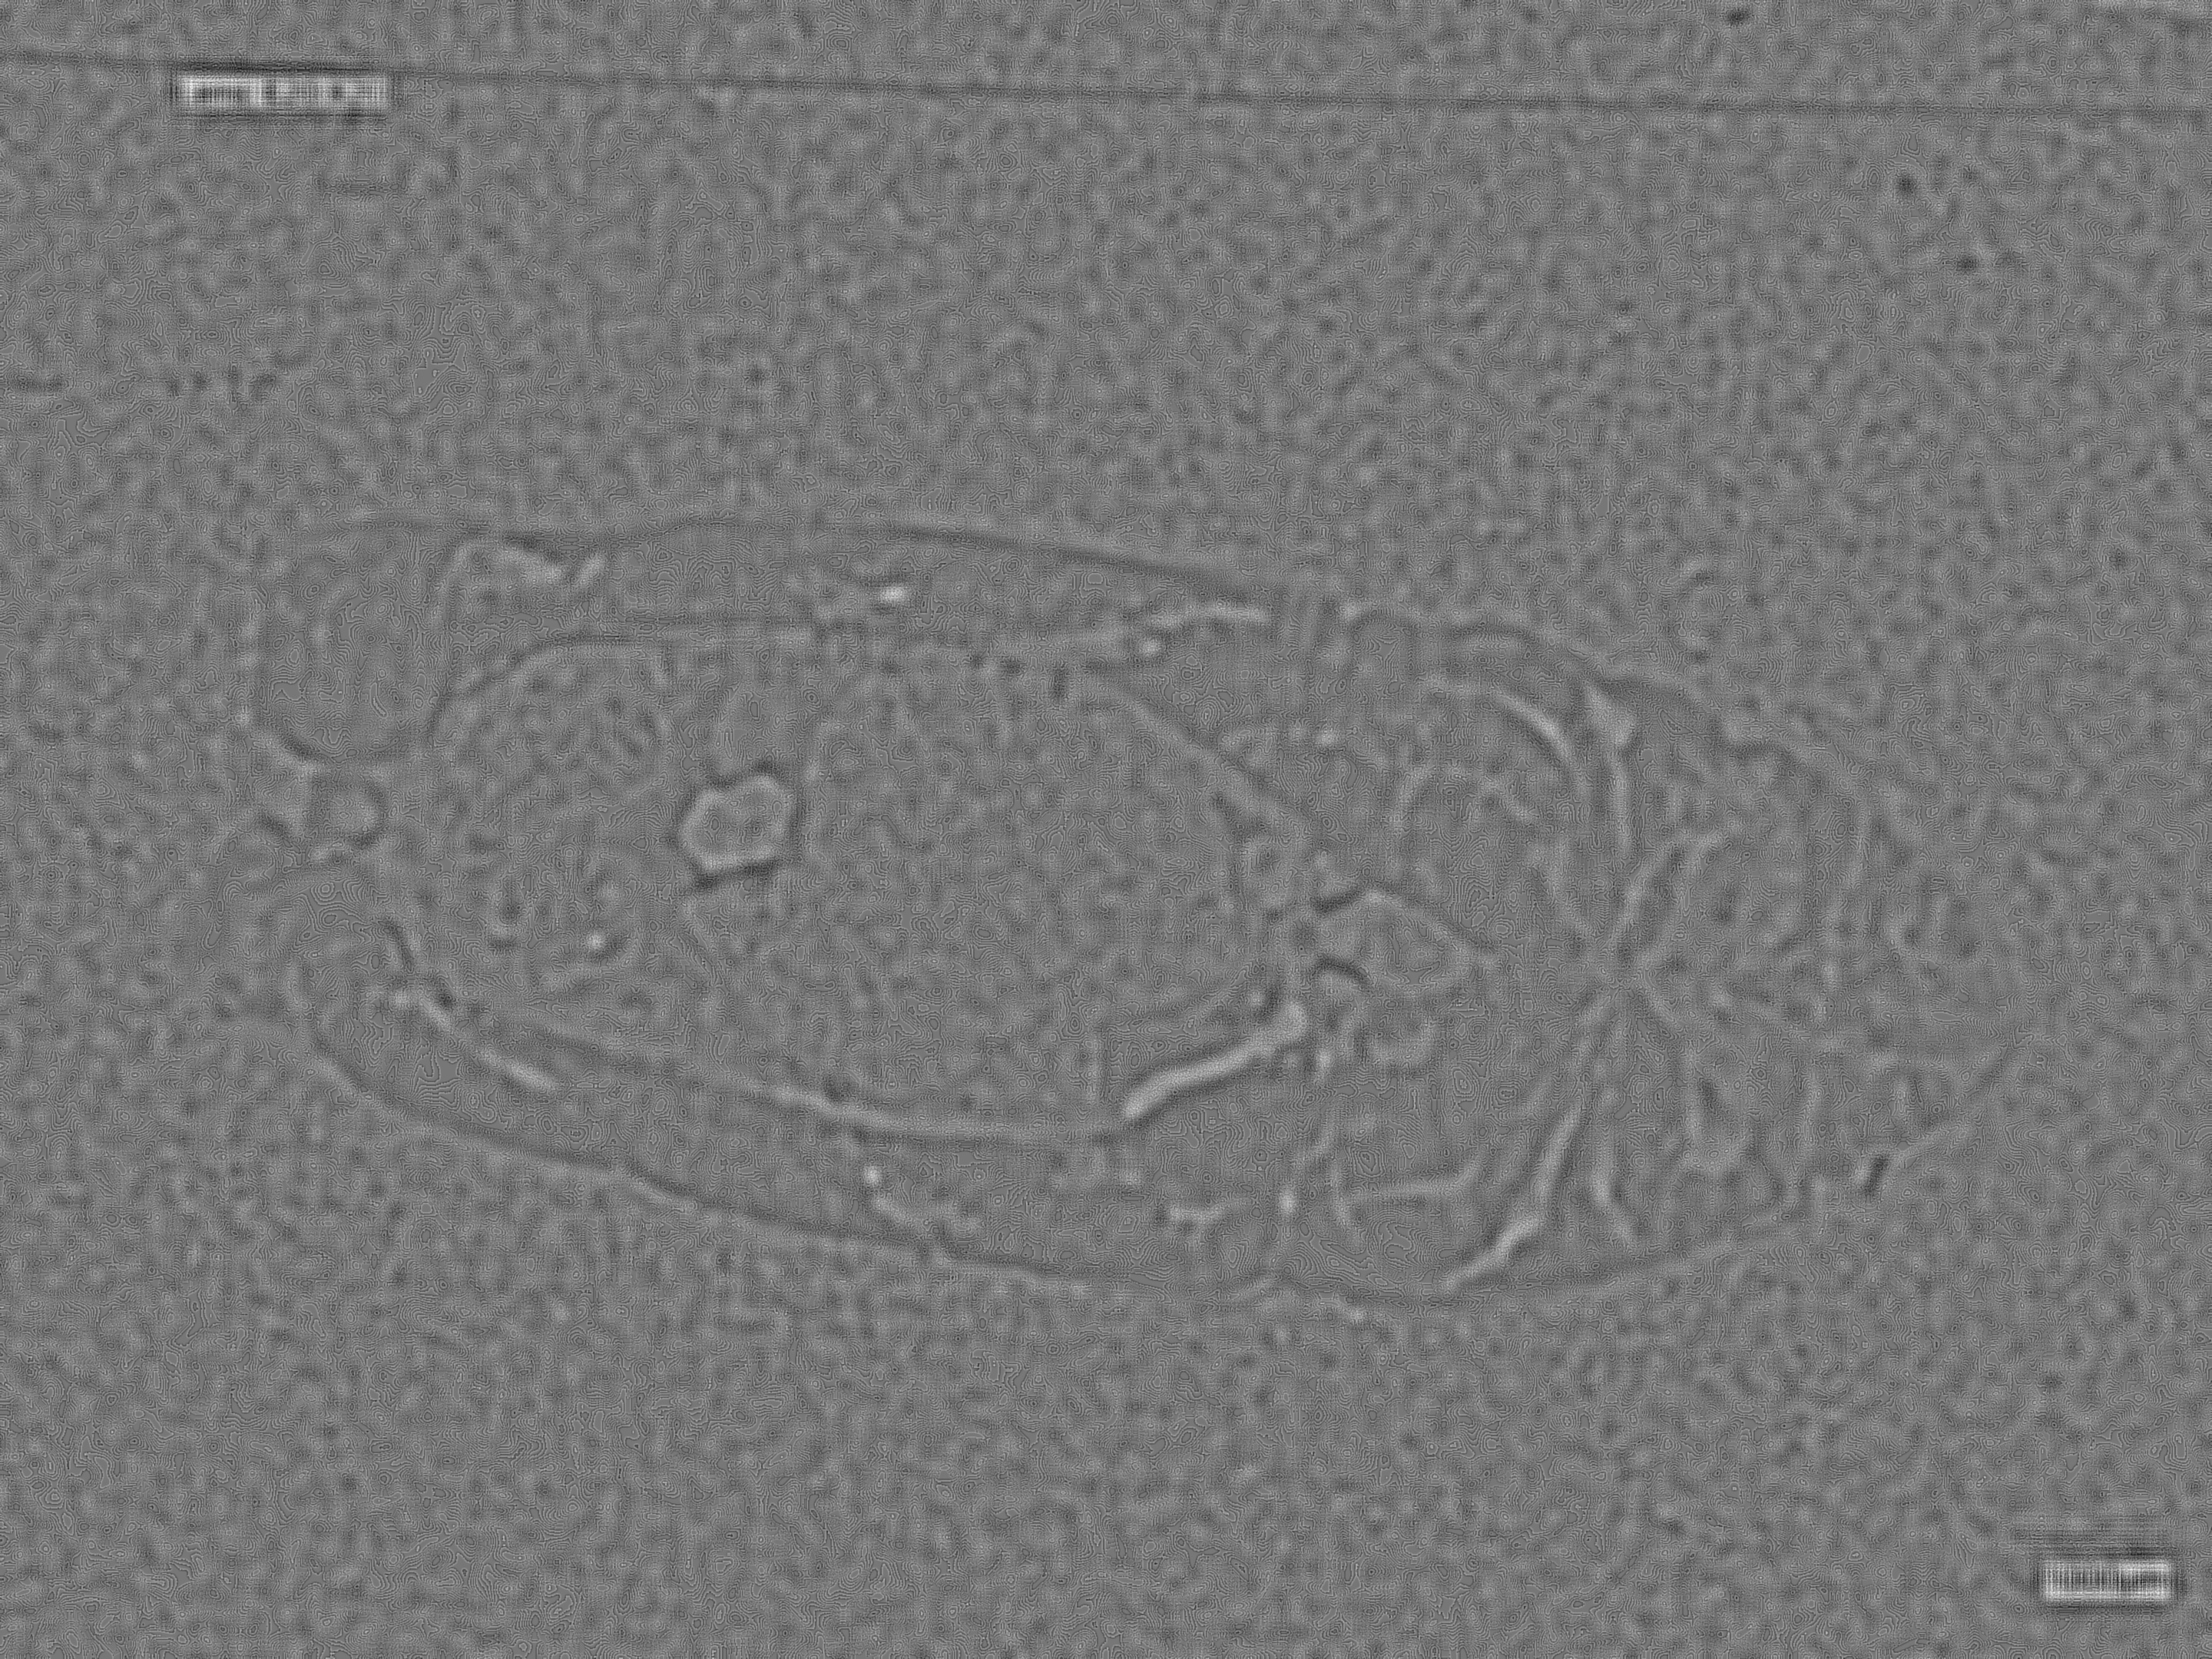
\includegraphics[width=0.45\textwidth]{./fig/gausssian/laplacian61.jpg}
\caption{Result of applying the Laplacian operator}
\label{fig:laplacian}
\end{figure}

As previously mentioned, the Canny algorithm is more sophisticated compared to the Sobel algorithm, incorporating steps such as thresholding and non-maximum suppression. The Canny method uses two thresholds, a low and a high. An image gradient greater than the high threshold is marked as an edge, while a gradient below the low threshold is not considered an edge. Gradients that are between the two thresholds are only considered edges if they are connected to high-threshold edges, effectively reducing noise and resulting in more accurate edge detection.

Typically, the ratio between the high and low thresholds is between 2:1 and 3:1. For this experiment, a ratio of 2.5:1 is selected, and the impact of different thresholds on edge detection is explored.

The chosen low thresholds are 2, 4, and 6, with corresponding high thresholds of 5, 10, and 15, respectively. The results of the Canny algorithm are shown below:

\begin{figure}
    \centering
    \begin{minipage}{0.32\textwidth}
        \centering
        \includegraphics[width=\textwidth]{./fig/gausssian/canny61+2.jpg}
        \caption{canny 2 5}
        \label{fig:canny2_5}
    \end{minipage}
    \begin{minipage}{0.32\textwidth}
        \centering
        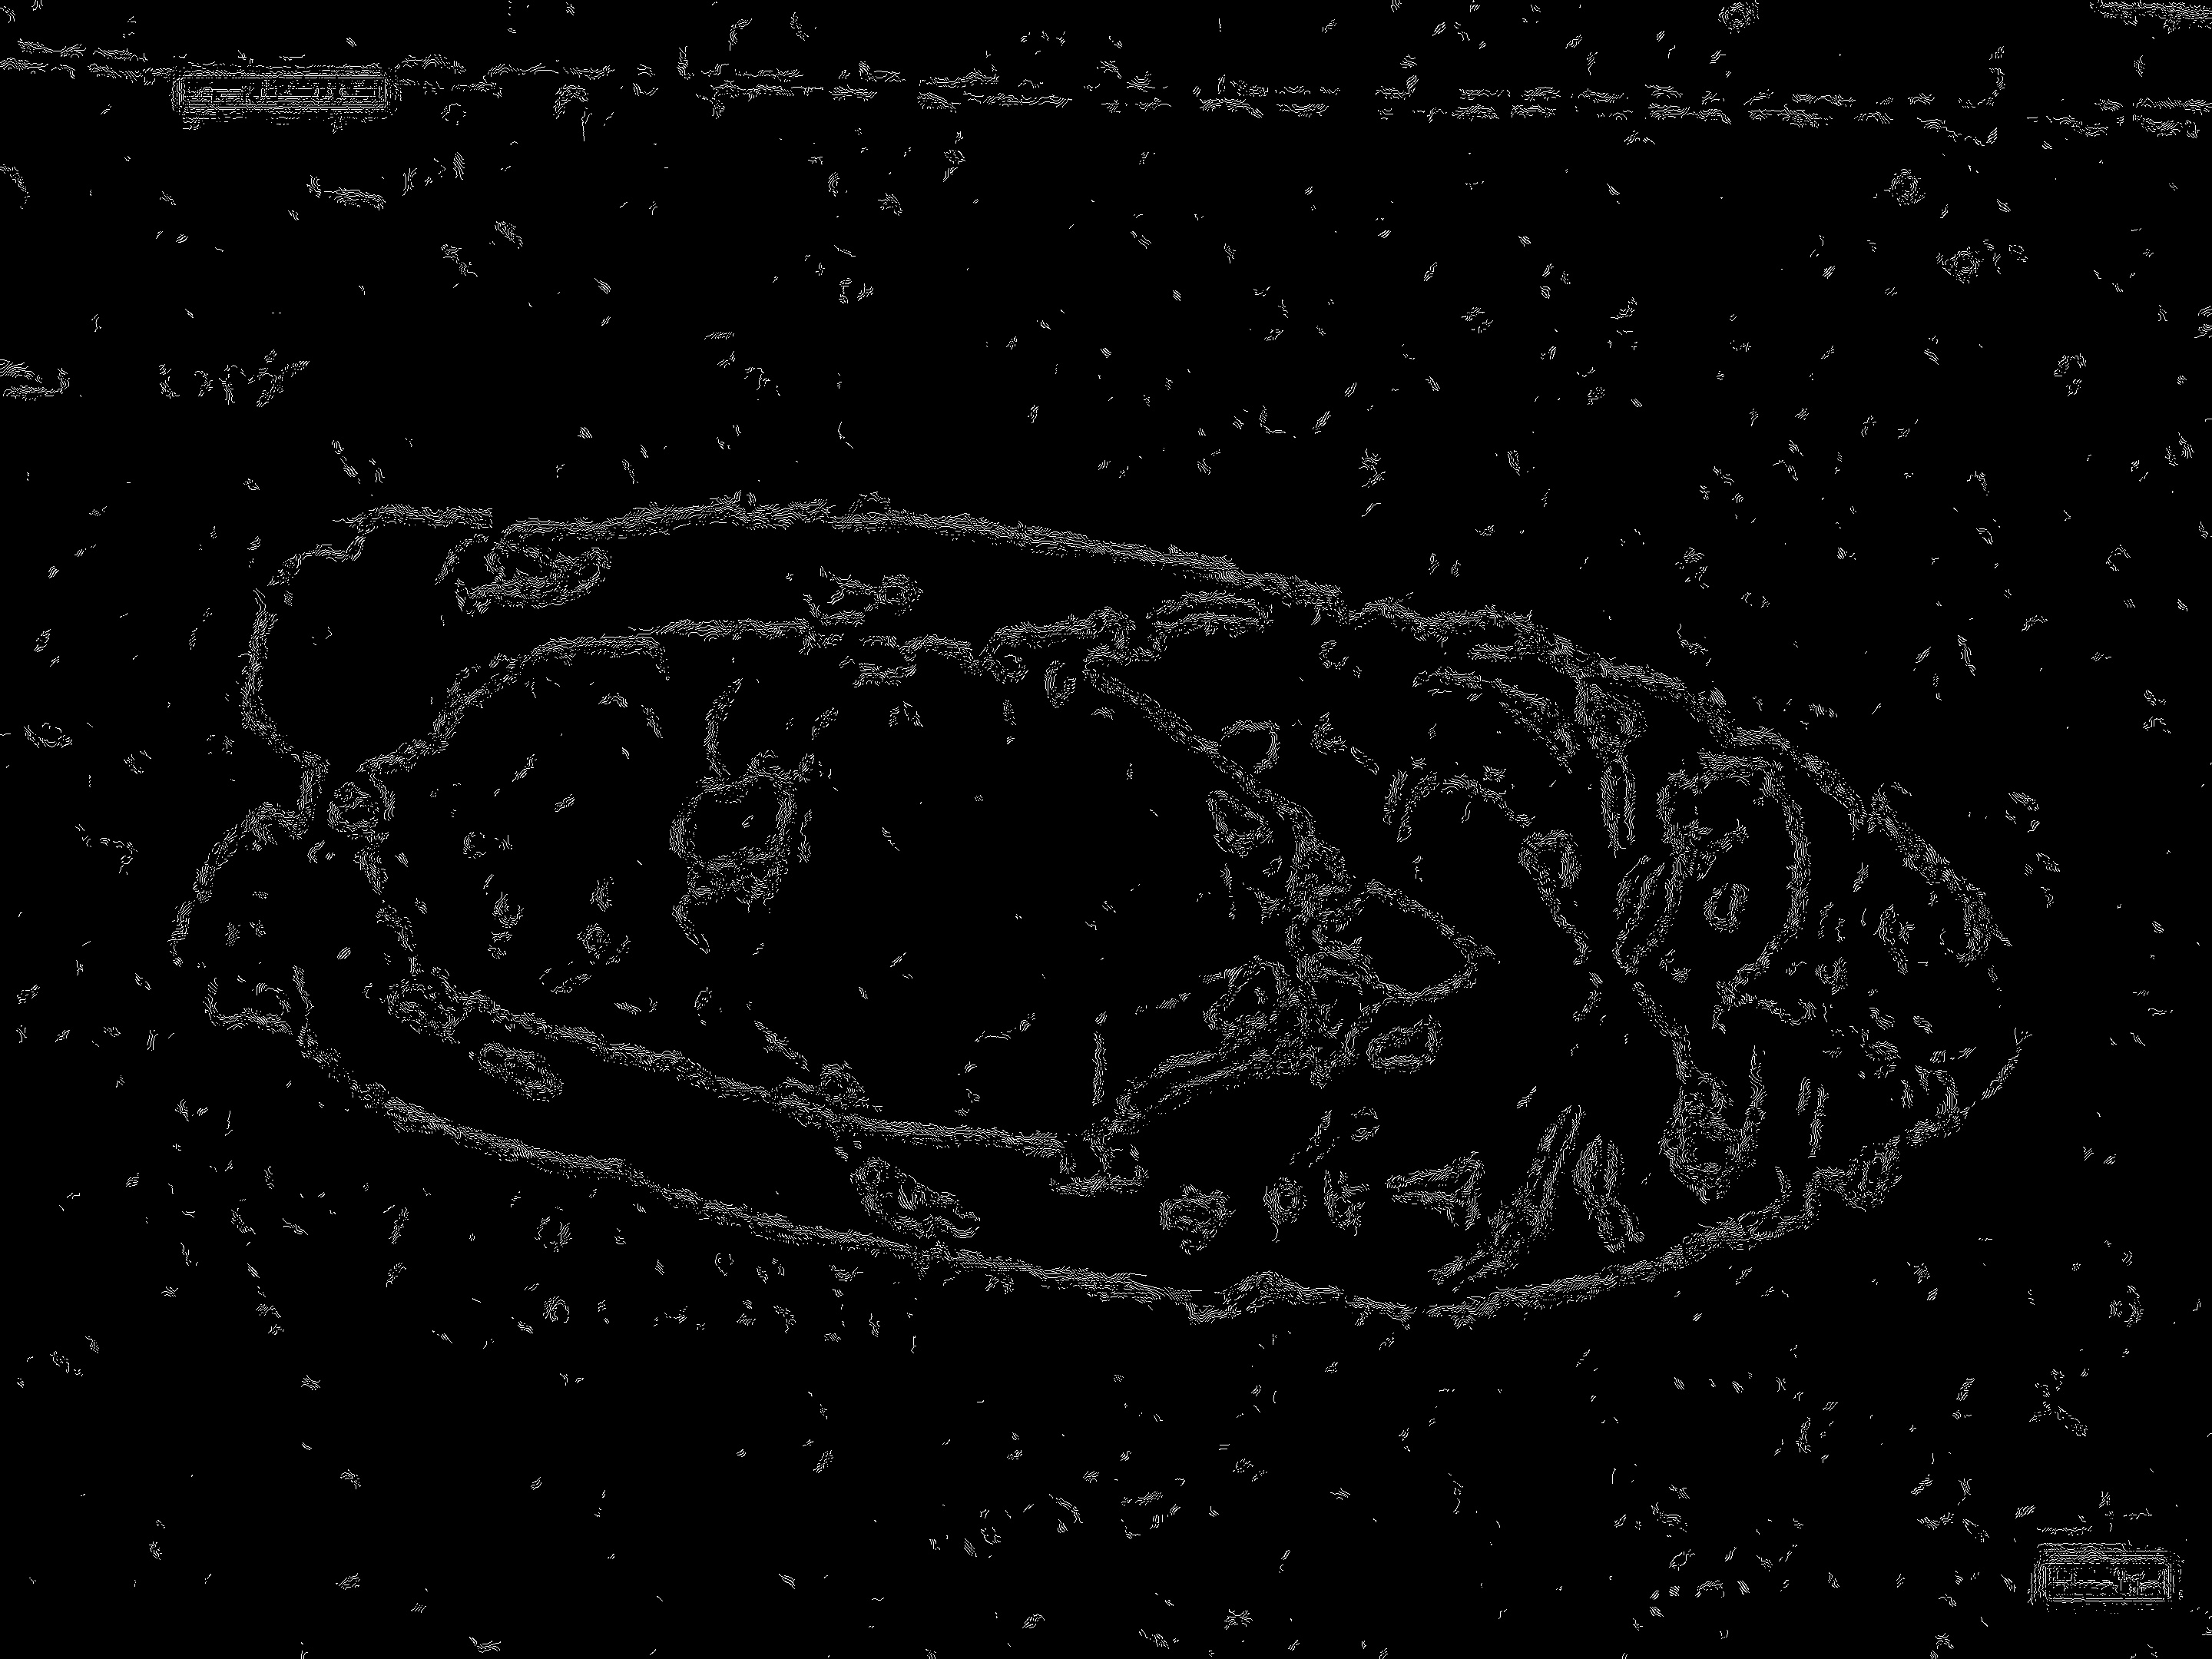
\includegraphics[width=\textwidth]{./fig/gausssian/canny61+4.jpg}
        \caption{canny 4 10}
        \label{fig:canny4_10}
    \end{minipage}
    \begin{minipage}{0.32\textwidth}
        \centering
        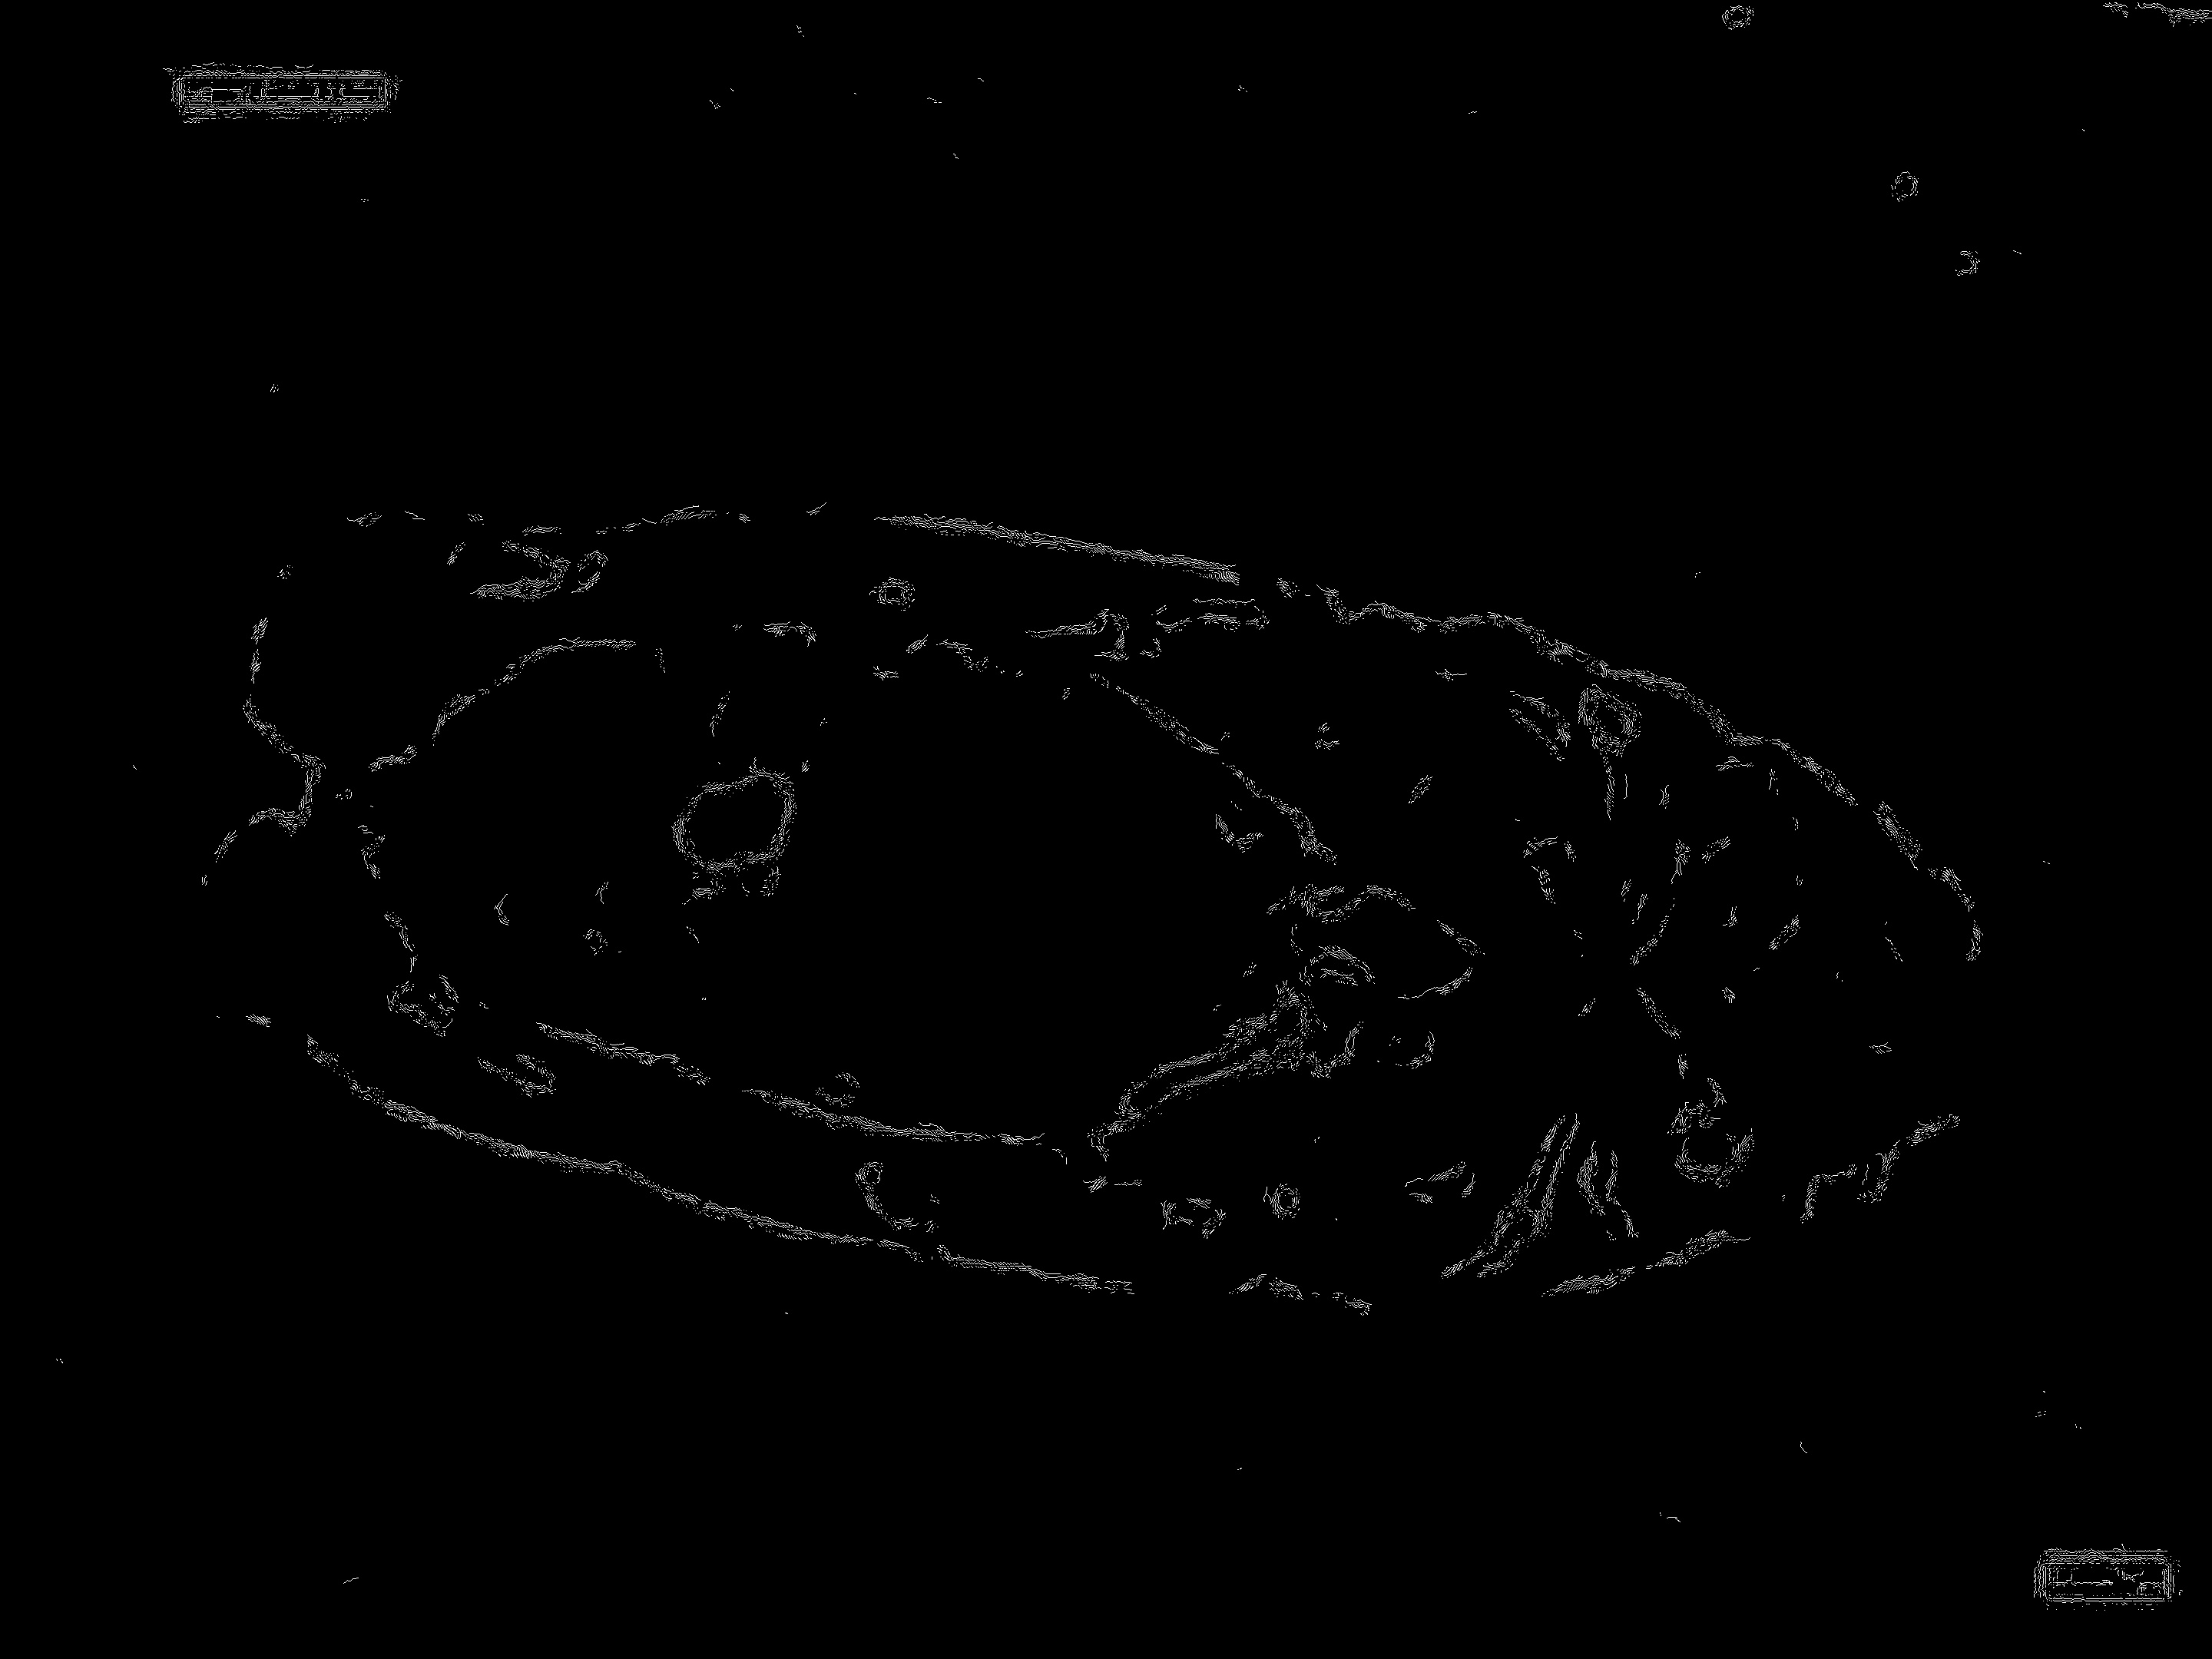
\includegraphics[width=\textwidth]{./fig/gausssian/canny61+6.jpg}
        \caption{canny 6 15}
        \label{fig:canny6_15}
    \end{minipage}
\end{figure}

Among the three Canny results, \autoref{fig:canny4_10} exhibits the best performance, managing to retain most of the edge details while effectively eliminating most of the noise. Consequently, the thresholds of 4 and 10 are chosen for the Canny algorithm.

\textbf{Summary}

Comparing the results of the Sobel, Laplacian, and Canny algorithms, the Sobel algorithm shows average performance, with significant edge detection but limited noise reduction. The Laplacian algorithm performs the worst, with edges becoming nearly invisible, likely due to its high sensitivity to noise. The Canny algorithm delivers the best results, maintaining edge details while effectively removing most noise. Therefore, the Canny algorithm is selected as the method for image preprocessing, enhancing the model's ability to focus on relevant features for further analysis.

\FloatBarrier


\subsubsection{Threshold Segmentation}

Considering the distinct colors of the biological tissue samples (yellow) and paraffin (white) in the specimens, threshold segmentation offers a straightforward method to distinguish between these two components by isolating the white regions of the image, leaving the biological tissue intact. This procedure involves enhancing the image contrast and saturation to better highlight the yellow color of the biological tissues, as demonstrated in \autoref{fig:enhanced_image}. The processing steps are executed using Python's OpenCV library.

Initially, each pixel in the image is evaluated, and pixels within approximately a radius of 15 (about 1\% of the image width) surrounding yellow pixels are preserved. Other colors are removed, as shown in \autoref{fig:yellowpic}. However, this method has shown limitations due to the dispersal of tissue fragments during the sectioning process, which can appear scattered throughout the specimen and interfere with the detection of yellow pixels.

\begin{figure}[H]
    \centering
    \begin{minipage}{0.45\textwidth}
        \centering
        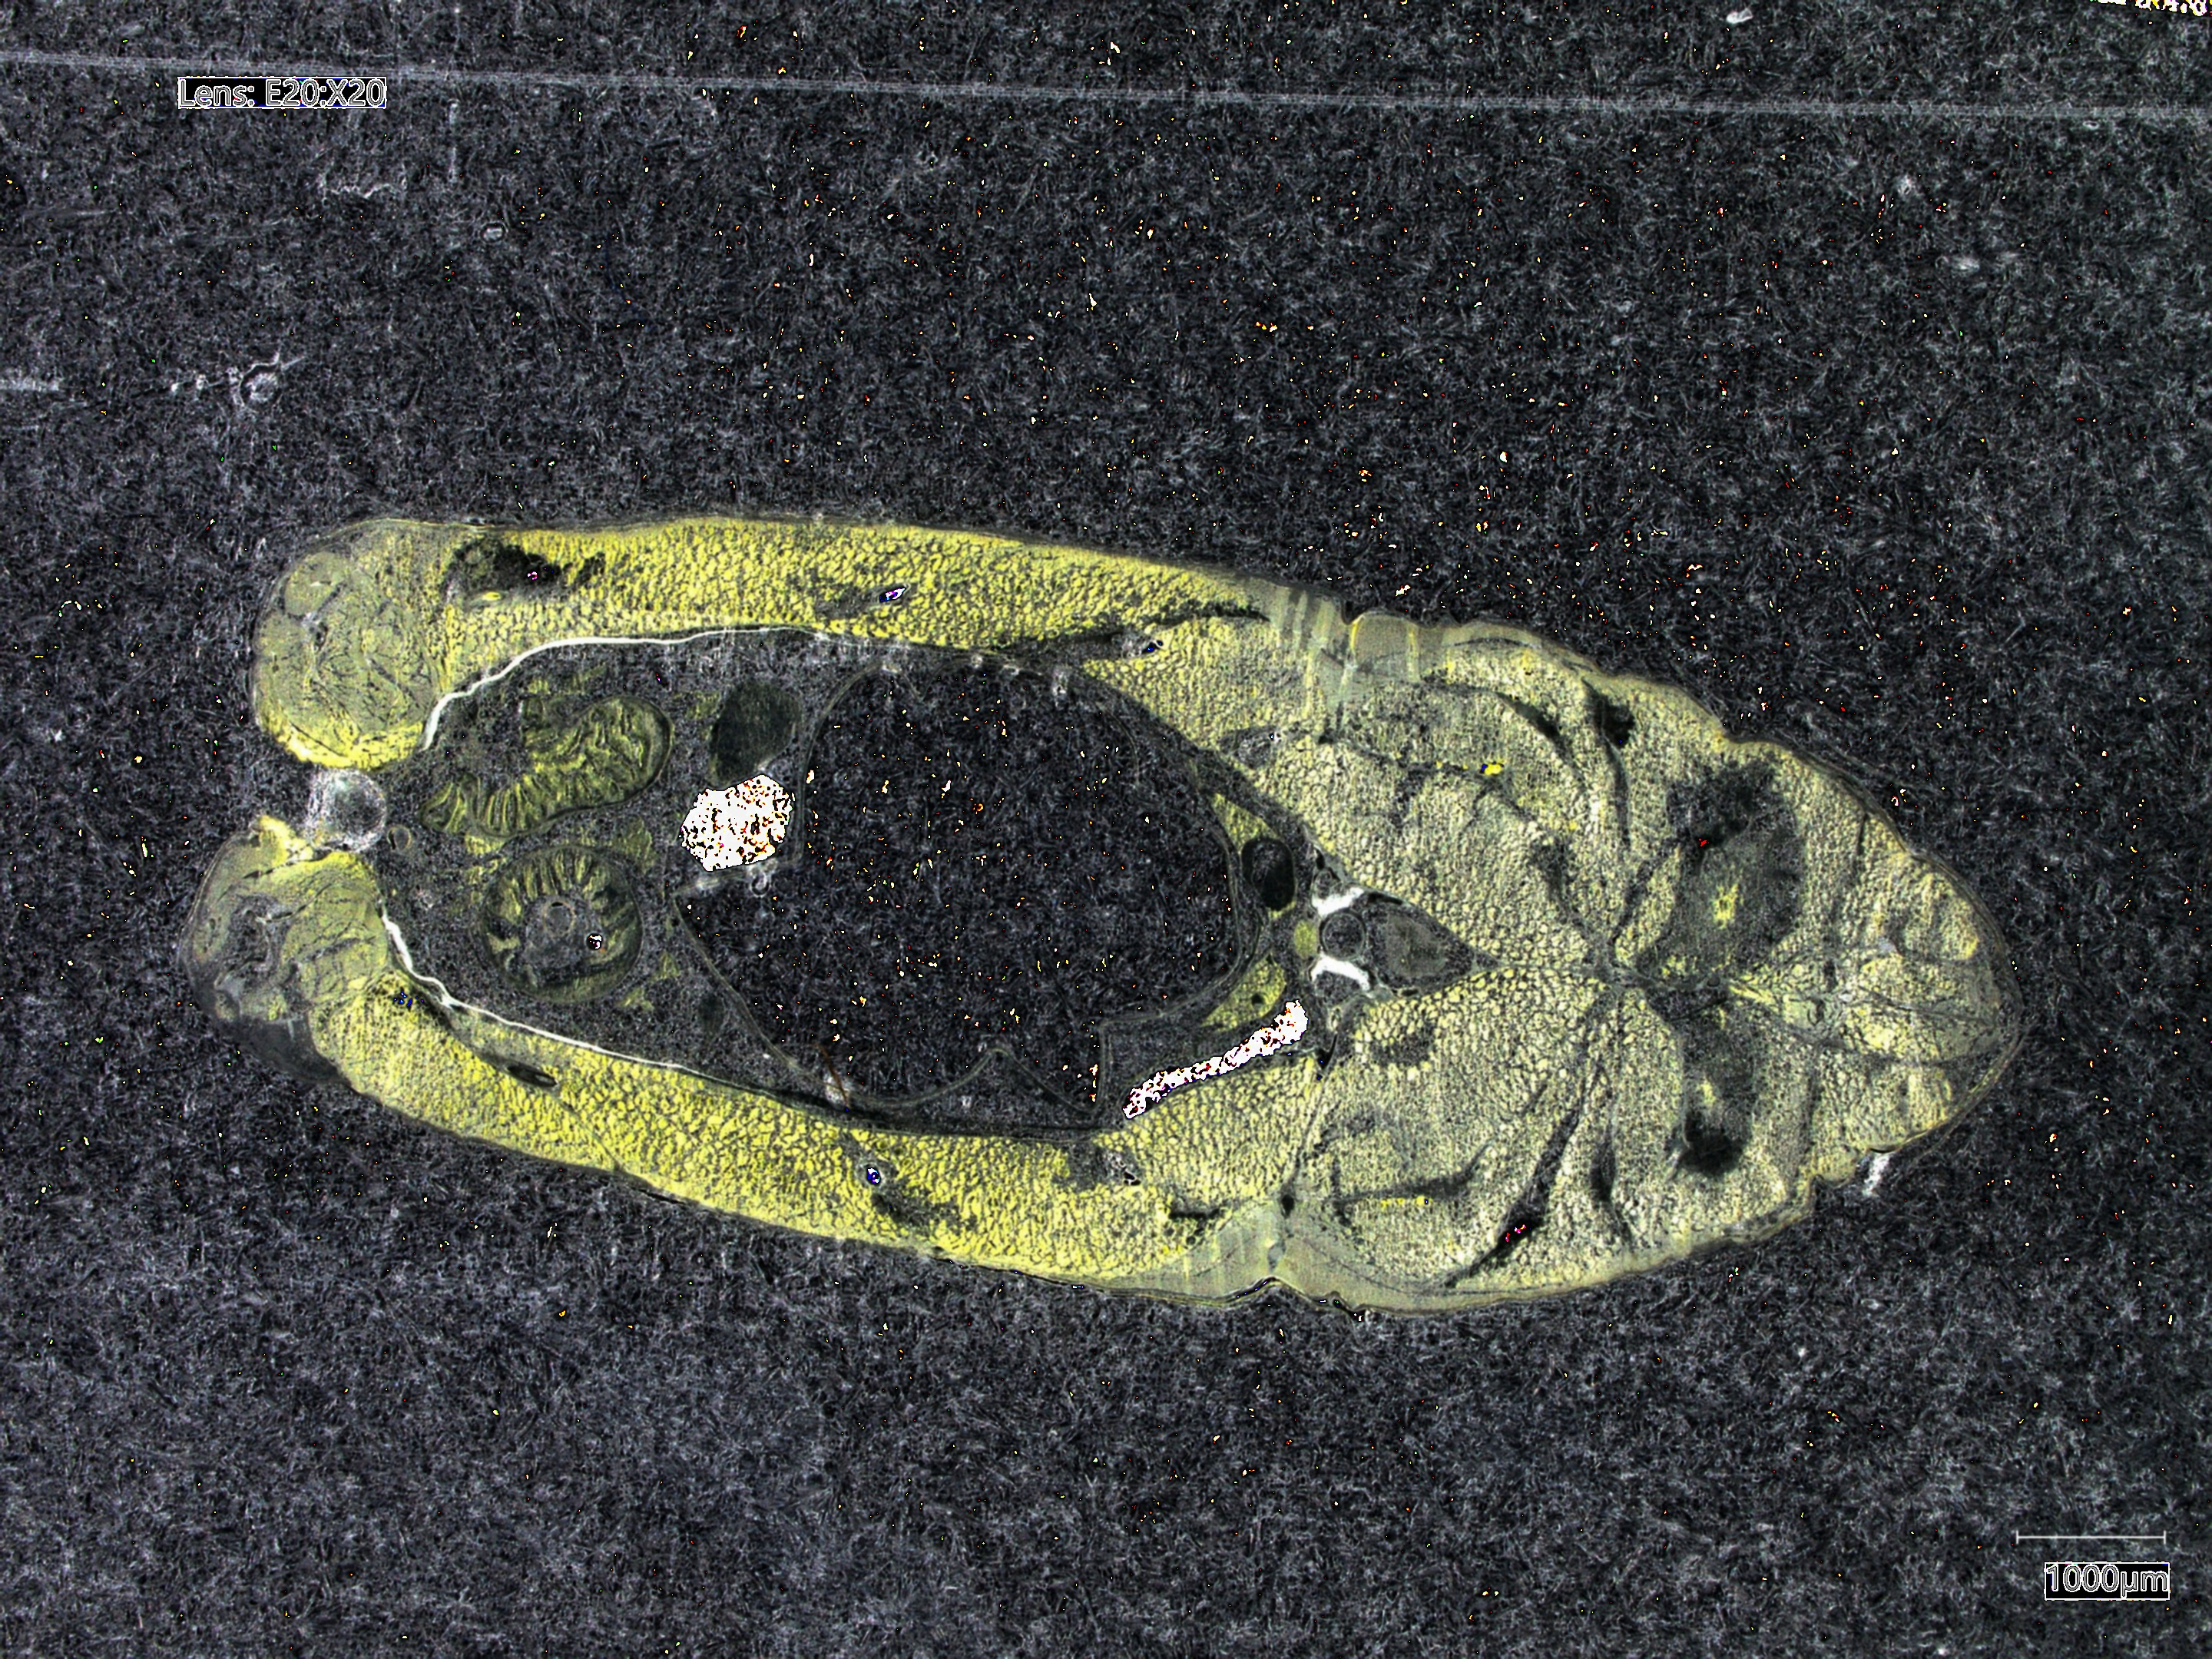
\includegraphics[width=\textwidth]{./fig/threshold/enhanced_image.jpg}
        \caption{Enhanced image for better color differentiation}
        \label{fig:enhanced_image}
    \end{minipage}
    \begin{minipage}{0.45\textwidth}
        \centering
        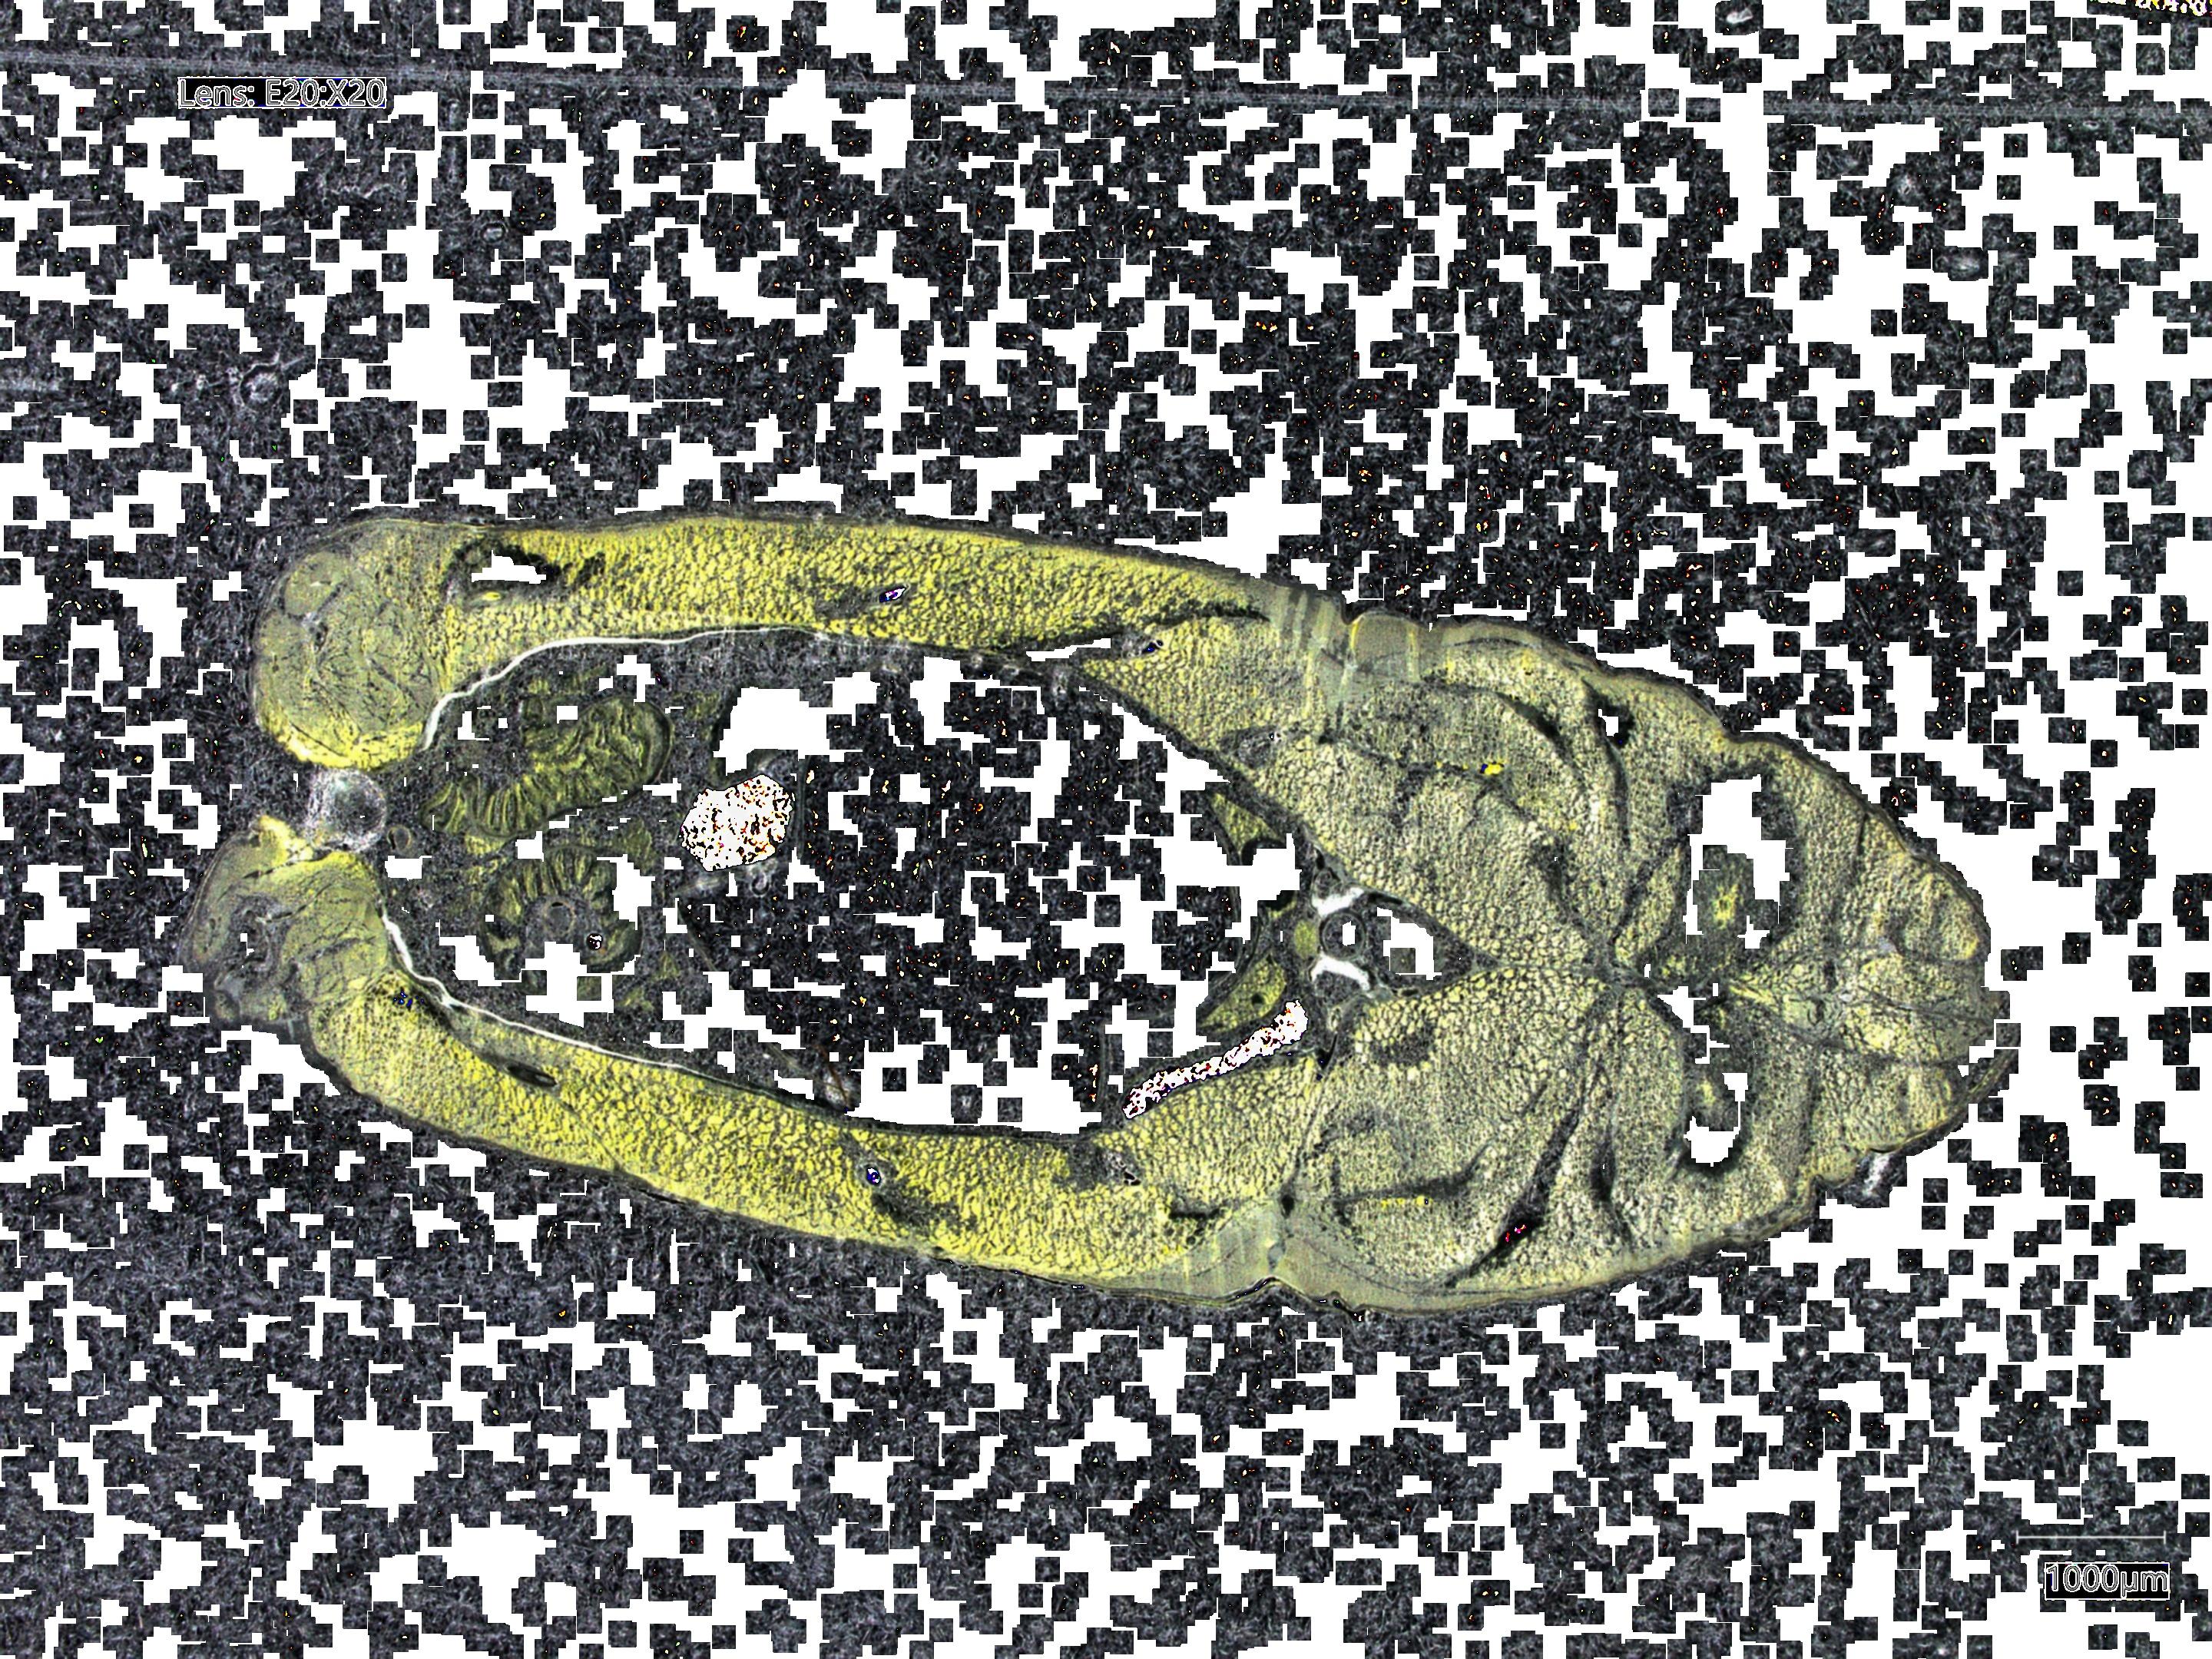
\includegraphics[width=\textwidth]{./fig/threshold/yellowpic.jpg}
        \caption{Segmentation focused on yellow pixels}
        \label{fig:yellowpic}
    \end{minipage}
\end{figure}

To refine the segmentation, further processing is required to eliminate black blocks appearing in the image. This is achieved by applying a mask inversion to turn these black blocks into white, thereby enhancing the separation of biological tissue from the paraffin base. The results are displayed in \autoref{fig:mask}.

\begin{figure}[H]
    \centering
    \begin{minipage}{0.45\textwidth}
        \centering
        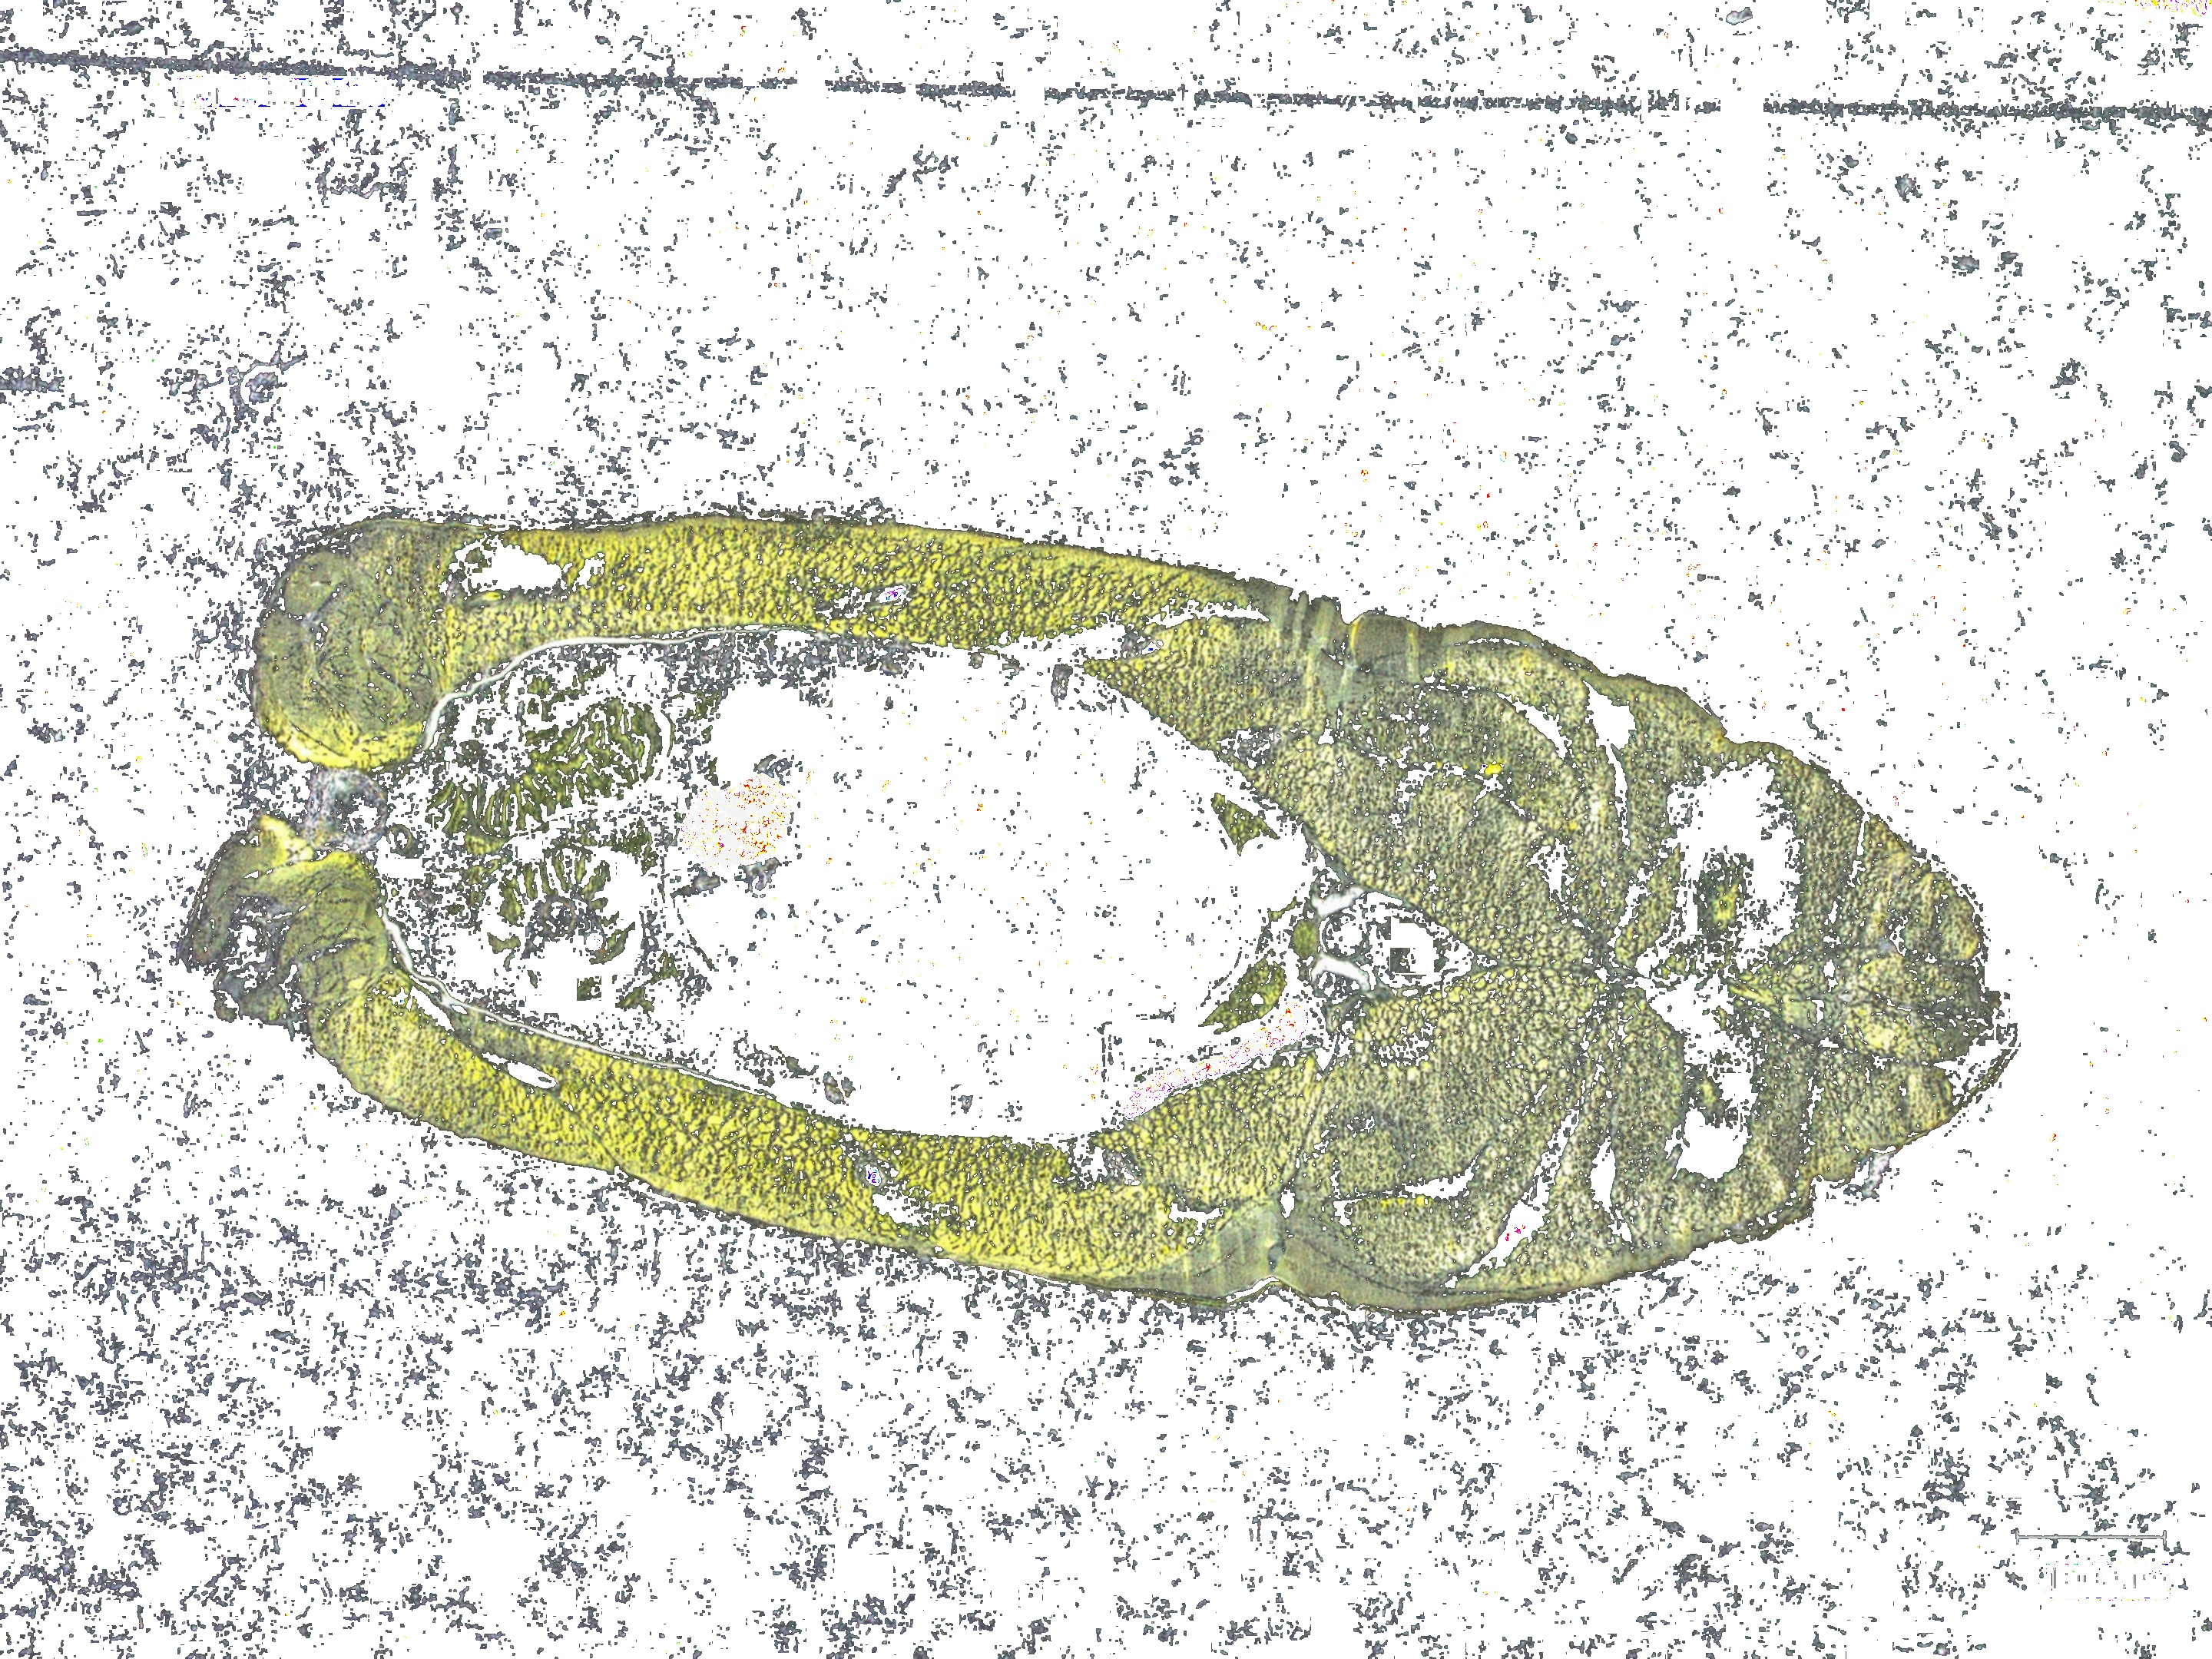
\includegraphics[width=\textwidth]{./fig/threshold/final.jpg}
        \caption{Final image after removing black blocks}
        \label{fig:mask}
    \end{minipage}
    \begin{minipage}{0.45\textwidth}
        \centering
        \includegraphics[width=\textwidth]{./fig/threshold/fingerprint.jpg}
        \caption{Result of segmentation using the fingerprint algorithm}
        \label{fig:fingerprint}
    \end{minipage}
\end{figure}

This approach demonstrates the utility of combining color enhancement and thresholding techniques to effectively segment biological tissue from paraffin in microscopic images. The challenge lies in accurately distinguishing tissue fragments from background noise and other non-tissue elements. This method can be particularly effective for automated image analysis in histopathology, where accurate tissue segmentation is crucial for research.

\subsubsection{Another Threshold Segmentation Method: Fingerprint Algorithm}
During the literature review, an article was found that described an improved segmentation method based on the Otsu algorithm, specifically adapted for fingerprint segmentation. Considering that both tissue sections and fingerprints are biological tissues with complex patterns and textures, it was hypothesized that this algorithm might also be effective for segmenting tissue sections. The results of applying this method are illustrated in \autoref{fig:fingerprint}.

The fingerprint algorithm, which is an adaptation of the Otsu method, is particularly effective in differentiating areas of high and low density, which is ideal for applications like fingerprint recognition where contrast between ridges and valleys is critical. The use of this algorithm in the context of biological tissue segmentation may offer a robust way to delineate regions of different cellular densities or structures within a sample.

\subsubsection*{Summary}

Based on the image preprocessing techniques discussed, both edge detection and threshold segmentation have shown promising results in highlighting the features of biological tissues and eliminating interference from paraffin. These preprocessing steps have significantly enhanced the visibility of essential features while minimizing noise and irrelevant information, which is critical for accurate analysis in histopathology.

To leverage these improvements, three datasets can be established:

\begin{itemize}
    \item Images processed through \textbf{edge detection.}
    \item Images processed through \textbf{threshold segmentation.}
    \item Images processed using \textbf{the fingerprint algorithm.}
\end{itemize}

These datasets will serve as training sets for the upcoming model training phase. Utilizing diverse preprocessing approaches not only enhances model robustness by providing varied representations of the data but also helps in exploring which image preprocessing technique best assists the model in learning relevant features effectively.
\FloatBarrier



\subsection{Model 2: Preprocessed Images with a Simple CNN Network}

In this section, we adapt Model 1c, the best-performing model from the previous experiments, to utilize preprocessed images. The architecture remains unchanged; however, the input now consists of images that have undergone various preprocessing techniques:

\begin{itemize}
    \item \textbf{Model 2a:} Utilizes images processed with Canny edge detection.
    \item \textbf{Model 2b:} Uses images processed through threshold segmentation.
    \item \textbf{Model 2c:} Inputs are images segmented using the fingerprint algorithm.
\end{itemize}

Each model follows the same architecture as Model 1c, which includes three convolutional layers each with 32 feature maps and 3x3 kernels, max pooling layers, and a fully connected layer with 256 neurons.

Results are displayed in the graphs below(\autoref{fig:model22_acc} and \autoref{fig:model22_loss}), showcasing the training and validation accuracy and loss for Models 2a, 2b, and 2c.
\begin{figure}
    \centering
    \begin{minipage}{0.49\textwidth}
        \centering
        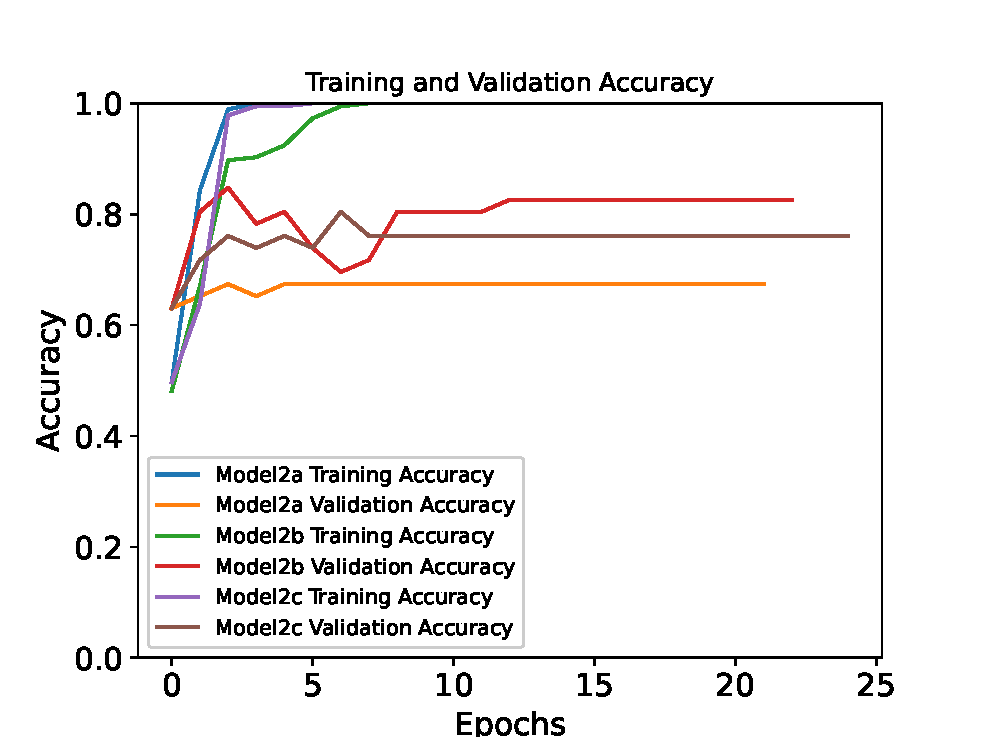
\includegraphics[width=\textwidth]{./fig/model2/accuracy22.eps}
        \caption{Accuracy of Model 2}
        \label{fig:model22_acc}
    \end{minipage}
    \begin{minipage}{0.49\textwidth}
        \centering
        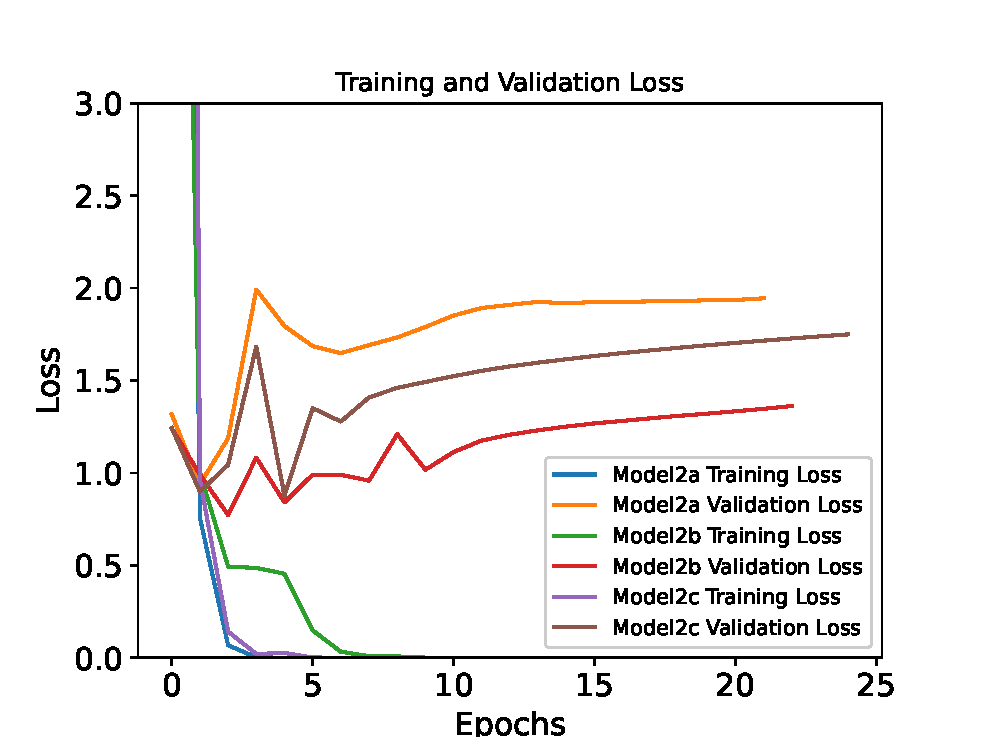
\includegraphics[width=\textwidth]{./fig/model2/loss22.eps}
        \caption{Loss of Model 2}
        \label{fig:model22_loss}
    \end{minipage}
\end{figure}


\subsubsection*{Summary}
The graphs illustrate that Models 2a and 2c begin to stabilize after approximately 8 training epochs, with training accuracies nearing 100\%, while validation accuracies stabilize around 65\% and 75\%, respectively. Despite high accuracies, both models exhibit relatively high validation losses above 1, suggesting overfitting and limited generalization to unseen data.

Model 2b, however, converges after about 10 training epochs, displaying the highest validation accuracy at approximately 82\% and a lower loss fluctuating between 1 and 1.2. This indicates that Model 2b performs better on the validation set, suggesting better adaptability and robustness. This might be due to Model 2b processing color images, which provide richer features from RGB channels, potentially enhancing feature extraction and generalization capabilities.

However, there is a risk that important details could be lost in the preprocessing steps, particularly with Model 2b's threshold segmentation. This can negatively affect the model's performance on specific types of images. An example of this loss of key information is demonstrated below:

\begin{figure}
    \centering
    \begin{minipage}{0.45\textwidth}
        \centering
        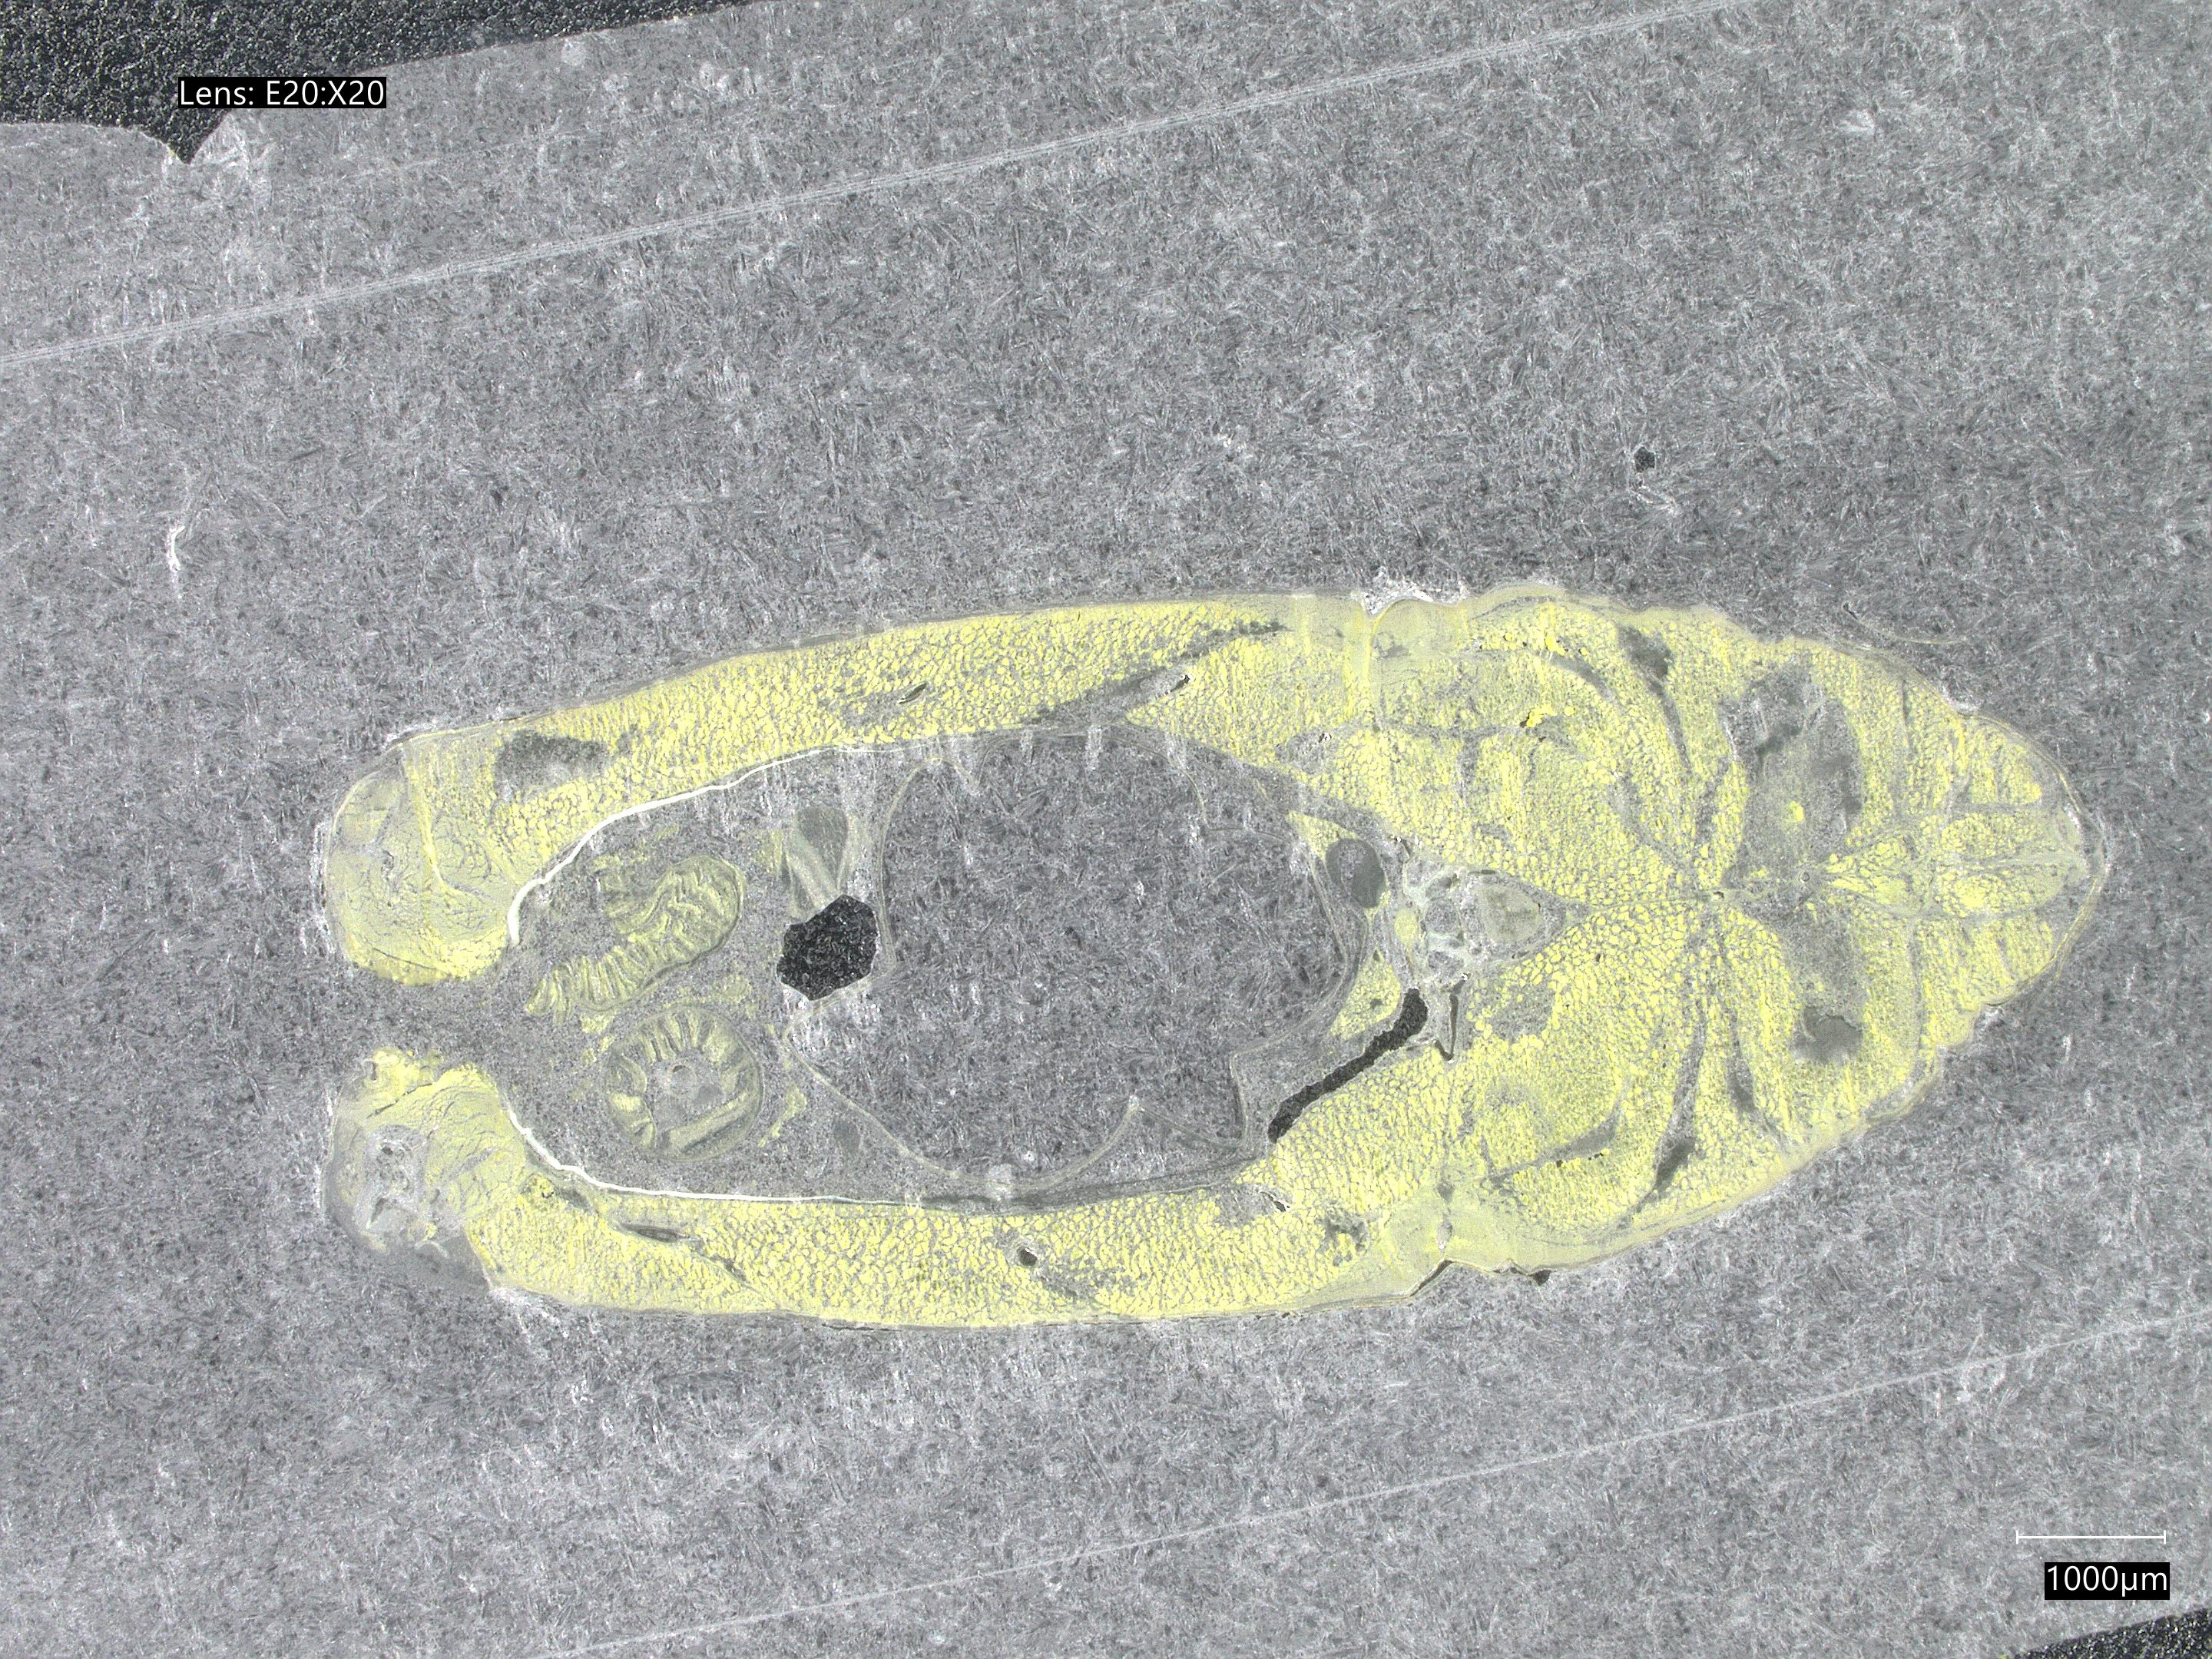
\includegraphics[width=\textwidth]{./fig/model2/origin20240205_161427.jpg}
        \caption{Original Image}
        \label{fig:origin}
    \end{minipage}
    \begin{minipage}{0.45\textwidth}
        \centering
        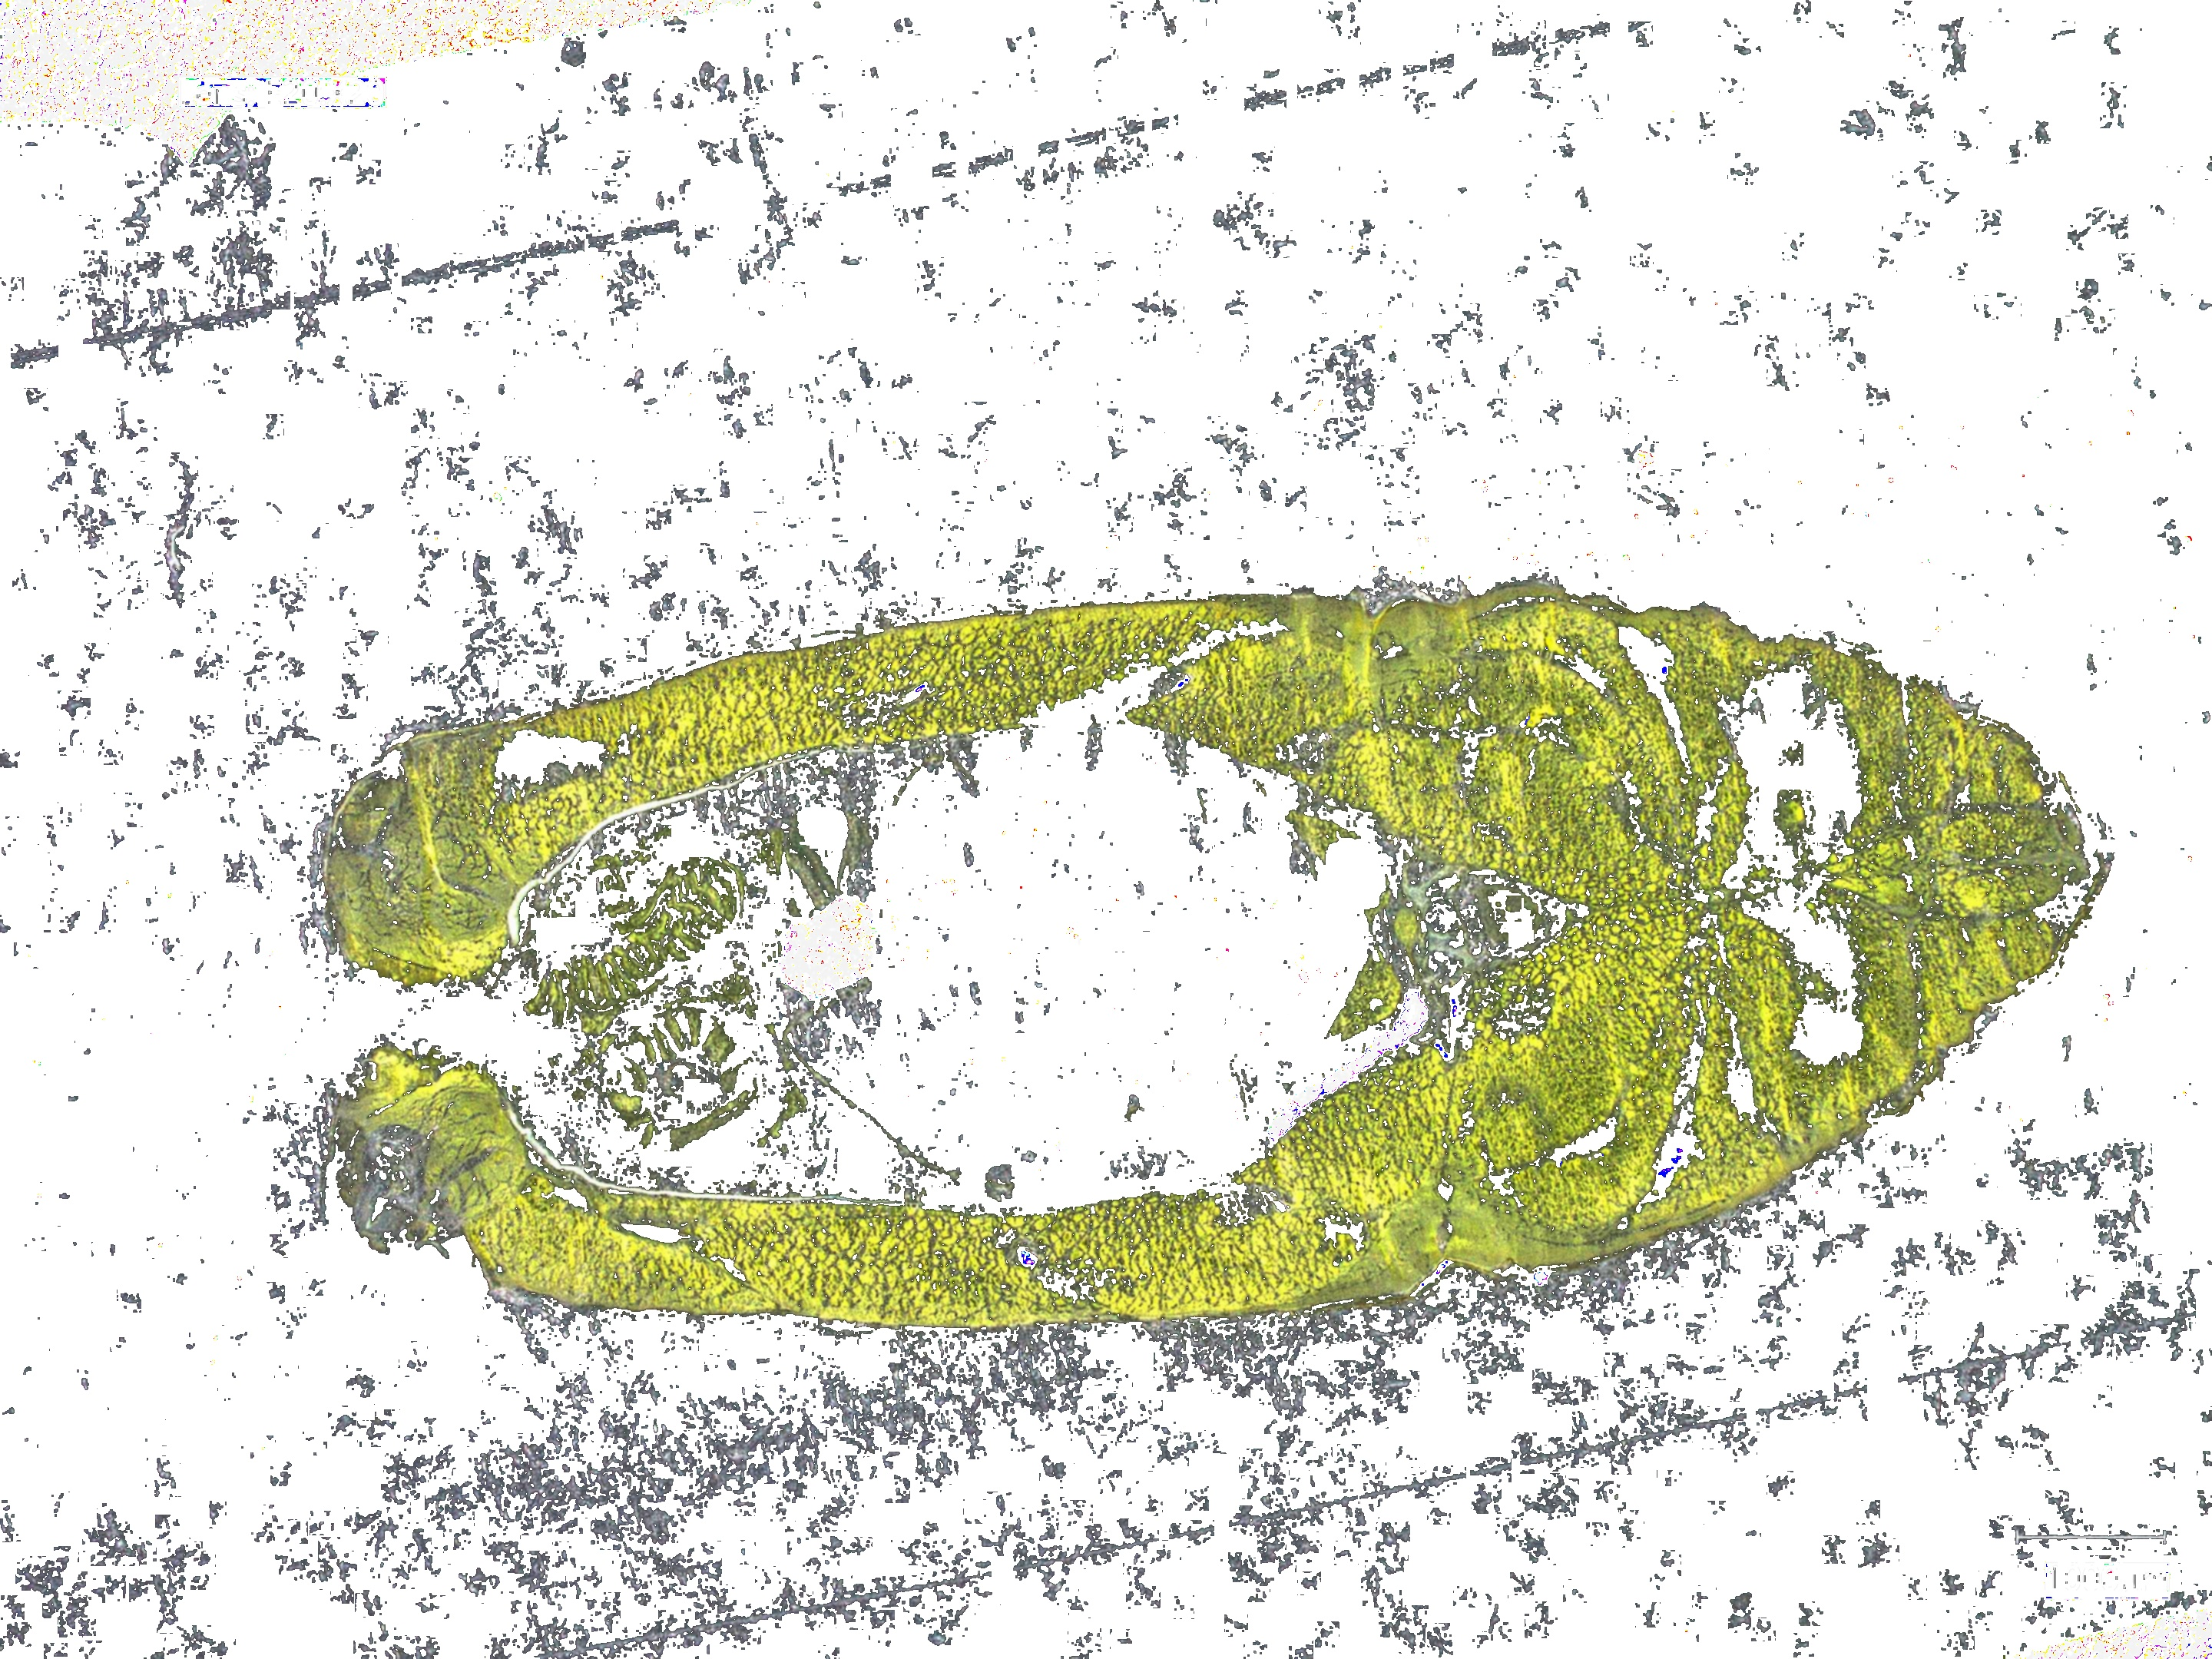
\includegraphics[width=\textwidth]{./fig/model2/yellow20240205_161427.jpg}
        \caption{Image after Yellow Threshold Segmentation}
        \label{fig:yellow}
    \end{minipage}
\end{figure}

In \autoref{fig:yellow}, we see that the threshold segmentation algorithm used in Model 2b’s training set significantly enhances horizontal creases, potentially confusing the model during training.

These findings highlight the challenges in image preprocessing. Aggressive preprocessing can sometimes eliminate crucial information, leading to diminished training outcomes. In future steps, transfer learning might be employed, utilizing pre-trained large-scale deep learning models adapted to our dataset, to improve training effectiveness and address these challenges.


\subsection{Model 3: Original Images with Transfer Learning}

\textbf{Transfer Learning with Pre-trained Models}

We are incorporating three well-known models pre-trained on the ImageNet dataset: VGG16, VGG19, and InceptionV3. These models come with pre-trained weights that are highly optimized and are expected to improve feature extraction capabilities significantly when adapted to our specific dataset.

\begin{itemize}
    \item VGG16 (Model 3a) and VGG19 (Model 3b) are similar, with VGG19 having three additional convolutional layers that could potentially offer better feature extraction capabilities.
    \item InceptionV3 (Model 3c) incorporates Inception modules that allow it to capture a broader range of features at multiple scales, providing a more complex and possibly more effective feature extraction mechanism.
\end{itemize}

\textbf{Adaptations for Transfer Learning}

To prevent overfitting and optimize the transfer learning process:

\begin{itemize}
    \item Early stopping is utilized.
    \item Learning rates are set low, at 1e-5 for VGG16 and VGG19, and slightly higher at 1e-4 for InceptionV3, given its more complex architecture.
    \item All models are adapted to accept an input size of 224x224, except for InceptionV3 which uses its default input size of 299x299. This uniform input size helps standardize the data preprocessing step.
    \item A global average pooling layer is added to each model following the base model layers, followed by a fully connected layer that matches the number of output classes.
\end{itemize}


\textbf{Observations from Model Training}

The training and validation performance of these models is depicted below:

\begin{figure}[H]
    \centering
    \begin{minipage}{0.49\textwidth}
        \centering
        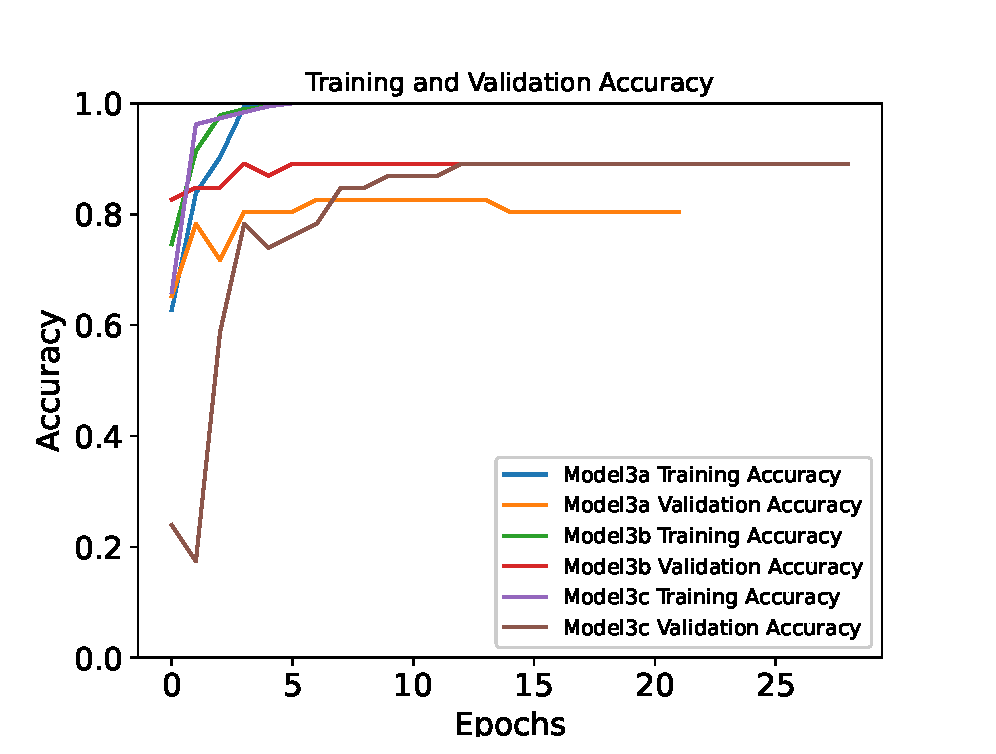
\includegraphics[width=\textwidth]{./fig/model3/accuracy33.eps}
        \caption{Accuracy of Model 3}
        \label{fig:model33_acc}
    \end{minipage}
    \begin{minipage}{0.49\textwidth}
        \centering
        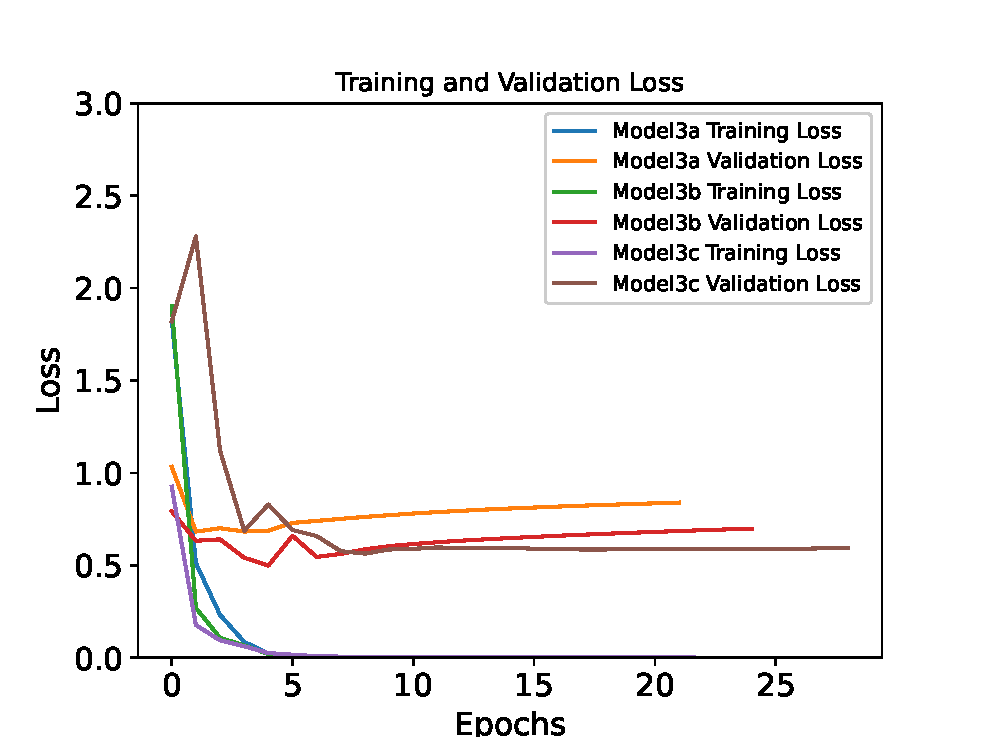
\includegraphics[width=\textwidth]{./fig/model3/loss33.eps}
        \caption{Loss of Model 3}
        \label{fig:model33_loss}
    \end{minipage}
\end{figure}

\textbf{Analysis}
\begin{itemize}
    \item Models 3b (VGG19) and 3c (InceptionV3) show significantly higher validation accuracies around 90\%, compared to Model 3a (VGG16).
    \item The loss metrics indicate that Model 3c (InceptionV3) has the lowest validation loss among the three, suggesting it is the most effective in generalizing to unseen data. This underscores InceptionV3's superior capability in capturing complex features.
    \item The performance gap between Model 3a and Model 3b supports the notion that the additional convolutional layers in VGG19 enhance its ability to process image features more effectively than VGG16.
\end{itemize}


\subsubsection*{Summary}

A comparative analysis of the VGG16, VGG19, and InceptionV3 models reveals that InceptionV3 yields the best training results, with both training and validation accuracies converging around 1 and 0.9 respectively, and losses converging around 0.6. This indicates that the InceptionV3 model not only trains effectively but also demonstrates superior generalization capabilities.

\subsection{Model Selection Summary}
When comparing across the model series—Model 1, Model 2, and Model 3—it is evident that Model 3 performs the best, particularly Model 3c. The underlying reason is likely due to Model 3's foundation on deep convolutional networks that are pre-trained on large-scale image datasets, enabling more effective feature extraction and development of a robust feature space.

\textbf{Notable Attributes of Model 3c (InceptionV3):}

\begin{itemize}
    \item \textbf{Architectural Design:} InceptionV3 features a modular design incorporating multiple "inception modules," which include multi-scale convolutional layers that operate in parallel within the same layer. This modular approach allows the network to capture a broad spectrum of features at various scales and depths.
    \item \textbf{Feature Extraction:} Inception modules can adaptively capture appropriate feature representations by processing different scales of features within the same layer. This adaptability makes it exceptionally capable of handling complex image data like biomedical images.
    \item \textbf{Deep Network Handling:} InceptionV3 integrates batch normalization and residual connections, which are critical in training deep networks. These techniques effectively mitigate issues related to vanishing gradients, thus facilitating the training of deeper models without performance degradation.
\end{itemize}

Given these advantages, Model 3c (InceptionV3) is selected as our final model for further applications and testing. This model stands out not only for its advanced architectural innovations but also for its proven effectiveness in generalizing well to new, unseen data, making it highly suitable for complex tasks such as medical image analysis where accuracy and reliability are paramount.

